\documentclass[a4paper,12pt]{article}
\usepackage[english]{babel}
\usepackage{setspace,graphicx,epstopdf,amsmath,amsfonts,amssymb,amsthm,versionPO}
\usepackage{marginnote,datetime,enumitem,subfigure,rotating,fancyvrb}
\usepackage[colorlinks=true,linkcolor=blue,anchorcolor=blue,citecolor=blue]{hyperref}
\usepackage[longnamesfirst]{natbib}
\usepackage{ctex}
\usdate
\usepackage{indentfirst}
\usepackage{Contatract}
\usepackage{multirow}
\usepackage{fancyhdr}
\includeversion{links}
\iflinks{}{\hypersetup{draft=true}}
\excludeversion{notes}	
\ifnotes{
  \usepackage[margin=1in,paperwidth=10in,right=2.5in]{geometry}%
  \usepackage[textwidth=1.4in,shadow,colorinlistoftodos]{todonotes}%
}{
  \usepackage[margin=1in]{geometry}
  \usepackage[disable]{todonotes}
}
\let\oldmarginpar\marginpar
\makeatletter\let\chapter\@undefined\makeatother
\newcommand{\rhs}[2][]{\smalltodo[color=green!30,#1]{{\bf RS:} #2}}
\newcommand{\rhsnolist}[2][]{\smalltodo[nolist,color=green!30,#1]{{\bf RS:} #2}}
\newcommand{\rhsfn}[2][]{
  \renewcommand{\marginpar}{\marginnote}
  \smalltodo[color=green!30,#1]{{\bf RS:} #2}
  \renewcommand{\marginpar}{\oldmarginpar}}
\newcommand{\textnote}[1]{\ifnotes{{\colorbox{yellow}{{\color{red}#1}}}}{}}
\newcommand{\clearRHS}{\clearpage\thispagestyle{empty}\cleardoublepage\thispagestyle{plain}}
\setcounter{tocdepth}{3}
\newtheorem{theorem}{Theorem}[section]
\newtheorem{assumption}{Assumption}[section]
\newtheorem{proposition}{Proposition}
\newtheorem{conjecture}{Conjecture}
\newtheorem{lemma}{Lemma}[section]
\newtheorem{corollary}{Corollary} \newtheorem{condition}{Condition}
\usepackage{endnotes}
\usepackage{color}
\usepackage{array}
\makeatletter
\def\enoteheading{\section*{\notesname
  \@mkboth{\MakeUppercase{\notesname}}{\MakeUppercase{\notesname}}}
  \mbox{}\par\vskip-2.3\baselineskip\noindent\rule{.5\textwidth}{0.4pt}\par\vskip\baselineskip}
\makeatother
\usepackage{lastpage}
\begin{document}
\selectlanguage{English}
\setlist{noitemsep}

\title{\color{black}  \begin{Huge}Contatract白皮书 \end{Huge} \\ [2ex] \begin{large}一个基于分布式存储的新一代功能完备的公有链项目\end{large}
\footnotetext{*作者:吴建刚。项目基金会为:Contatract Foundation Ltd.,它是一家注册于新加坡的非营利性组织。网站:https://contatract.org。E-mail: contatract@gmail.com。
  }}

\author{吴建刚$^*$}


\date{2020年1月 V0.5}
\renewcommand{\thefootnote}{\fnsymbol{footnote}}
\singlespacing
\maketitle
\thispagestyle{empty}
\vspace{-.2in}

\renewcommand\abstractname{\large{摘要}}
\begin{abstract}
  \noindent

按照卡尔达舍夫的文明等级划分标准,人类文明仅为0.7,还不足I型文明。面对原始丛林,人类单个个体是脆弱无力的;面对浩瀚宇宙,人类作为整体也是脆弱无力的。人类文明的升级离不开大规模的深度合作,而要达成这种合作就需要使人类个体之间能够跨越地域、制度、组织甚至国家等的障碍进行高效的交流和交易。

互联网的出现极大的促进了人们的交流和交易,但现有的互联网普遍是建立在中心化的服务器基础上的,并且随着互联网巨头的崛起,规则制定权和数据使用权被中心平台控制,限制了互联网进一步发展。现有互联网与最初人们设想的平权的互联网理想渐行渐远。

互联网未来发展总的趋势是从中心化向分布式发展。区块链的出现极大的促进了分布式资源提供者一起合作提供存储、带宽、支付等服务。但是,目前的区块链应用由于缺乏\textbf{可读写的分布式存储}和\textbf{可扩展的分布式记账},其应用范围受到极大的限制。目前的区块链主要应用在转账、存证、博彩等,存储和记账除了世界状态(所有矿工共同保存的交易数据)这一效率低下的功能外,无力处理大规模交易和大数据存储,这大大限制了区块链应用的普及。

本项目的正是为了解决这两方面的问题,一是构建可读写的分布式存储,二是构建可扩展的分布式记账。

关于可读写的分布式存储,区块链最需要的是一个“可编程”的世界硬盘,使分布式应用能够基于此建立文件系统和数据库系统,从而建立复杂的应用。因此,本项目的存储架构与IPFS的设计完全不同,本项目的分布式存储提供的是一个可读写的“裸盘”,任何用户可以使用私钥控制自己的分布式云空间,并在其上建立自己的文件系统和基于文件的数据库系统,从而为区块链系统提供那块“缺失的硬盘”,并使分布式系统的开发者可以用它建立各种实用的DApp。这也可能是对互联网的基础架构的重大变革,从而对互联网产生深远的影响。

关于可扩展的分布式记账,本项目的分片机制不仅能够进行交易分片,还能进行数据分片,是真正的无限可扩展的记账机制。该记账机制的共识机制结合了PoS抵押机制、PBFT出块机制和PoW选举机制,形成对系统的多重保障,具有极大的安全性。

分布式通讯也是分布式系统必须具备的功能,但它是附加在分布式存储功能上的,所以没有分布式存储来得重要。因为,有了分布式存储,分布式通讯系统的建立就变得容易了。信息交流,不论是两人会话还是多人会话,不论是文字、语音还是视频,对于各类交易在事前、事中和事后都是异常重要的。传统区块链缺乏可读写的分布式存储空间,难以建立分布式通讯系统,而本项目拥有分布式存储功能,通讯数据可以通过分布式云作为中转,从而实现真正的点对点的分布式通讯功能。

本项目利用区块链分布式记账技术为分布式存储网络提供时空证明机制和付费机制,并以此系统为基础将信息互联网与价值互联网进行整合,从而构建了去中心化的新一代互联网系统——分布式互联网——的技术框架。\textbf{项目名称“Contatract”(交子链)来源于:\underline{Conta}ct+Con\underline{tract}}(以下简称“CNT”),其寓意是要通过区块链整合分布式的交流和交易,帮助人们高效合作。而交子币则是用于交流和交易的币子。该公有链以可读写的分布式存储为基础,备且无限可扩展交易能力,可以在上面建立我们日常所见的各类应用的分布式版本,\textbf{是一个真正的区块链3.0项目}。

我们认为实现点对点转账功能的比特币是第一代区块链,它主要是通过激励机制组建分布式系统;实现了智能合约功能的以太坊是第二代区块链,它主要通过图灵完备的虚拟机实现了可编程的转账;而类似Contatract的公有链拥有分布式存储、无限可扩展的交易、分布通讯等功能,是\textbf{功能完备的区块链},可以在上面建立功能完备的DApp,可以被认为是第三代区块链。

本项目将服务对象界定为DApp开发者,只有赋权开发者,才能激发创造热情,形成良好的生态。为了形成完整的开发工具和导入最初的用户,Contatract基金会将同时开发Contatract公链上第一款DApp——Wemore,意寓着“We together can create more”,或“为陌”,意寓着“通过为陌生人服务让自己过上更幸福的生活”。Wemore是一个基于Contatract公链的分布式云服务和分布式电子邮件服务提供者。在中心化互联网时代,电子邮箱和云服务都是杀手级产品,在分布式互联网时代同样如此,\textbf{分布式云服务和分布式电子邮箱极可能成为分布式互联网时代的杀手级产品}。

实际上,Wemore只是一款演示产品,它告诉人们区块链可以实现分布式交易、分布式存储和分布式通讯,而拥有这些功能的像Contatract这样的功能完备的区块链几乎可以被应用于任何涉及交易、存储、通讯的场景,并拥有让传统App无缝过渡到DApp的能力。由于任何应用场景都涉及数据存储、通讯和交易,而这些功能可以很容易嵌入到现有的App中,使其有可能逐步转化成分布式应用。由于App都有法币接入,这使各国的人们可以利用法币向应用商购买分布式云存储,而应用商可以利用法币代为购买CNT,这使CNT不仅可以用于传统应用,还使传统客户更容易获取到区块链服务。

综上述,Contatract以解决可读写的分布式存储和可扩展的分布式记账为基础,实现了分布式通讯,从而使区块链从图灵完备进化为功能完备的区块链,通过为开发者提供完备的功能,让信息互联网和价值互联网无缝地整合为新一代的分布式互联网,从而可能极大的提高人们相互交流和合作的能力。

\end{abstract}

\medskip
\noindent
 \\\\
\medskip
\noindent

\thispagestyle{empty}

\newpage
\thispagestyle{empty}

\noindent
\textbf{\large{使用申明:}}

任何人在未经许可的情况下,出于非商业或教育用途(即收费或商业用途除外),均可使用、复制或分发本白皮书,前提是引用了原始来源和适用的版权声明。

免责声明:本Contatract白皮书仅供参考。 Contatract基金会不保证本白皮书的准确性或达成的结论,本白皮书仅是“按照现在的样子”提供。Contatract基金会不作或明确地否定任何明示或暗示的、法定的或其他方面的陈述或保证,包括但不限于:(1)本白皮书的内容没有错误;(2)这些内容不会侵犯第三方的权利;(3)适用于特定目的、适用性或作用的保证。对于因使用、参考或依赖本白皮书或此处包含的任何内容而引起的任何形式的损害,即使被告知有此类损害的可能性的情况下,Contatract基金会及其关联公司不承担任何责任。在任何情况下,Contatract基金会及其附属公司均不对任何个人或实体因以下事件承担任何形式的责任:损害、损失、责任、成本或费用,无论是直接的还是间接的、后果性的、补偿性的、偶然的、实际的、惩戒性的,或者使用、引用或依赖本白皮书或其包含的任何内容造成的包括但不限于业务、收入、利润、数据、功能、商誉或其他无形损失的任何损失。


\medskip
\noindent
 \\\\
\medskip
\noindent

\thispagestyle{empty}

\newpage
\thispagestyle{empty}

\noindent



\vspace{-2in}
Love and knowledge, so far as they were possible, led upward toward the heavens. But always pity brought me back to earth. Echoes of cries of pain reverberate in my heart. Children in famine, victims tortured by oppressors, helpless old people a burden to their sons, and the whole world of loneliness, poverty, and pain make a mockery of what human life should be. I long to alleviate this evil, but I cannot, and I too suffer.
\singlespacing

\begin{flushright}
--Bertrand Russell
\end{flushright}

\newpage
\setcounter{page}{1}
\pagenumbering{Roman}
\renewcommand{\contentsname}{\centerline{目\  录}}
\tableofcontents
%\thispagestyle{empty}

\newpage

\clearpage

\onehalfspacing

\setcounter{footnote}{0}
\renewcommand{\thefootnote}{\arabic{footnote}}


\setcounter{page}{1}
\pagenumbering{arabic}


\pagestyle{fancy}

\lhead{Contatract以促进人类交流和交易为己任}
%\chead{}
%\rhead{}
%\lfoot{}
\cfoot{}
\rfoot{\thepage\ of \pageref{LastPage}}%当前页 of 总页数
%\renewcommand{\headrulewidth}{0.4pt}%改为0pt即可去掉页眉下面的横线
%\renewcommand{\footrulewidth}{0.4pt}%改为0pt即可去掉页脚上面的横线



\section{项目背景与目标}
\subsection{人类文明发展的动力、现状和困境}                    

单个人的力量是微不足道的,人类文明的进步源于人类合作的广度和深度。人类合作进步主要受益于制度进步和技术进步。制度主要指与各类组织相关的制度,技术则主要是指与人类交流和交易有关的技术。

人类合作的基础方法是分布式市场。基于分布式市场的社会分工协作是人类合作的最基础和自然的方法,市场机制的巧妙被亚当.斯密喻为“看不见的手”而加以赞扬。但是,人类的合作面临信息不透明、信息不对称、观念冲突和大脑缺乏程序接口等障碍,完全分布式的市场在解决信任问题上,能力是有限的,所以,社会发明了各种中心化组织来解决信任问题。当前,人类合作的制度主要是围绕中心化组织(国家、宗教、企业等)建立的。随着互联网的发展,人的交流与合作越来越多可以在线进行,契约的成本也大大减少。类似谷歌、苹果、脸书、腾迅、阿里这样的互联网平台,作为在线合作时代新的中心化组织,在人类在线合作中起着重要的作用。

中心化组织为人类文明做出了极大贡献,但是也给文明带来了各种阻力和重大风险。各类中心化组织在地理、文化、宗教、制度、信息系统等方面越来越中心化,不仅造成交流和交易的障碍,也成为各种冲突的主要来源。中心化组织越强大,组织之间的隔阂和对抗就可能越严重,组织内的压迫也可能越明显,组织失败的影响也越大。世界大战、地区冲突、贸易保护、企业垄断使人类合作受到极大的影响,并可能止步不前。

中心化组织在解决信任问题时也面临单点风险、阶层分化和组织冲突等困境。所谓,中心化组织的单点风险,是指中心化组织越成功就造成越多的权力、资本、人才和数据集中于少数机构或少数人手里,一旦这些机构被外部攻破或内部变节,后果都不堪设想。其次,资源占有在越来越集中在少数人手里还造成组织内形成不同的阶层,阶层冲突难以避免,相互压榨也是屡见不鲜。最后,组织内部各种增加凝聚力的方法,被称为爱国主义、企业文化、宗教信仰等等方法,恰好使组织之间的观念冲突难以避免,加上组织之间信息不透明,使组织之间的信任问题也难以解决,甚至使残酷的竞争成为常态。

从大的时间尺度看,人类文明还处在非常初级的阶段。由于人类文明只能使用故乡行星上部分能源,在物质层面主要使用微米级材料,所以根据卡尔达肖夫指数计算,目前人类文明处于0.73型文明\citep{sagan2000},即人类文明仍然仅属于0型文明的范畴。可以说,人类面对浩瀚宇宙是异常脆弱的,就象在襁褓里的孩子。但这样正需要长身体的孩子却被中心化组织带来的局限扼住了喉咙。

不得不指出,当前中心化方案显示的弊端还在继续扩大,在互联网时代表现得尤为明显,让人类的发展陷入某种困境。互联网刚出现时,我们看到互联网在信息传播和媒体透明上起到重要的作用,但随着互联网的发展,各种基于中心化的互联网平台也形成了寡头垄断,大型互联网平台的数据越来越多的集中在少数中心化组织手里,流量垄断、数据垄断、技术垄断越来越严重,使大量的个人或小企业只能依附于少数大型集团,同时小的创业公司越来越难以成功,这对于人类创新已经构成极大的障碍。基于大型互联网平台的人类合作在互联网发展的第一阶段极大地促进了人类文明进步,但随着互联网发展的深化,互联网的权力越来越不平等,并造成平台对资源的垄断。

\subsection{区块链的兴起及带来的希望}                    

2008年11月1日中本聪发表的比特币白皮书,让人类实现了通过网络发行私人货币这一创举,而其背后的区块链技术在解决合作主体之间的信任问题上极具潜力,这正是区块链被《经济学人》的封面文章称为“信任的机器”的原因。现有大部分技术主要促进了“生产力”的进步,而区块链是对人们的“合作方式”的革新,是对生产关系的技术革命。在区块链出现之前,人类的合作只能通过中心化的方案,体现在互联网就是使用中心化服务器,建立在TCP协议上的C/S或B/S架构。区块链让我们看到了把中心化交易撮合平台转化成分布式撮合平台的可能,这样做既能将分布式市场经济的效率发挥到极致,又能避免中心化组织带来的问题,从而极大的减少分布式市场的信任成本。事实上,针对人类合作不透明、非理性、观念冲突和缺乏程序接口等主要障碍,区块链都能给出合理的分布式的解决方案,主要原因是区块链拥有分布式记账、共识机制和代币激励、基于地址和私钥控制的资产、智能合约、可信数据、分布式通讯等特点。

区块链带来最大变化的行业首先是金融。比特币开创了非政府发行货币和无中介电子转账,2017年的ICO热潮则让我们看到了各种资产通过代币化实现数字化、分布式记账和可编程的广阔前景。可以想象,未来包括证券、土地、房产、汽车、石油等各种资产都将大量被映射到链上,从而实现资产数字化、分布式记账和可编程。

但未来,如果区块链能够实现分布式存储和分布式通讯,区块链就有潜力组建分布式互联网的基础设施,从而为人类基于中心化组织的合作转向分布式组织的合作提供无限的可能。第一代互联网是中心化信息互联网,已经给社会带来了极大的改变,而正在崛起的分布式信息互联网和价值互联网是互联网发展的深化和必然趋势。

更为重要的是,在人类历史上第一次,区块链给人类核心问题,即信任问题的一个分布式的解决途径,即将信任交付给代码。基于区块链的智能合约替代了纸质合约,不仅使契约的自动化执行成为可能,还使陌生人之间可以基于对代码的信任进行交易。通过分布式记账和智能合约让人类可以不依赖中心化机构实现分布式市场交易的自动化,让人类从走出非洲以来第一次在合作技术上实现质的飞跃,从此人类合作将逐步进入到2.0时代,即建立在分布式互联网基础上的人类组织和合作。可以预见,基于区块链的分布式技术将逐渐解决中心化组织的弊端,扳开扼在人类喉咙上的中心化组织的魔咒,开启了人类文明通往更高级阶段的新旅程。

\subsection{区块链当前的缺陷和要解决的问题:从图灵完备到功能完备}

区块链在支付领域的应用是从2009年的比特币开始的,作为图灵完备的区块链的以太坊的提出是从2014年,但到目前为止,除了比特币和以太坊有超过100万级用户外,其它区块链应用基本没有达到这个数量级的,日活则更少,只有几十万,但中心化的应用用户达到千万的比比皆是,上亿的也不鲜见。区块链项目不仅缺乏杀手级应用,在各行各业中也较少落地。我们可以从中心化平台与公有链平台的比较中获知一二。一个中心化平台一般都有注册和身份认证、数据存储、通讯、下单交易等功能,平台在可扩展性和用户体验上也更胜一筹。而区块链在这些功能上,几乎不是空缺就是极不完善。以下列出区块链功能主要几个不完善的方面。

\begin{enumerate}
\item 扩容。扩容是指区块链交易的确认效率,目前比特币的TPS平均不到10笔,以太坊平均不到20笔,EOS速度以超级节点的能力也仅达到上百。目前,区块链扩容通过分片、分层和共识机制几个方面在努力,但都还不成熟。
\item 存储。互联网的发展是伴随着数据存储技术而发展的,但目前区块链基本采用数据块向全网广播,不仅效率低下,还很难产生各种基于数据的应用。IPFS虽然给出了一定的文件存储的思路,但对于高频读写的数据是没办法依赖IPFS实现的。
\item 通讯。目前重要的应用,不管是爱彼迎、优步还是淘宝都内置通讯功能,更不要说社交类应用了,这是因为大部分交易在交易前、交易中和交易后都有通讯的要求。目前的区块链正在建立价值互联网,但却未能将信息互联网的功能整合起来,而未来的区块链项目需要能够可以高效地整合人类的交流和交易的系统化的解决方案。
\item 跨链。我们期待区块链能够将大量的价值上链表示,并通过区块链形成价值互联网,但目前看来,各个区块链形成了自己的价值交互,但区块链之间却很难进行价值交互,这实际上形成了区块链的群岛,但却没有岛与岛之间的联系。为此,现在已经产生上万家交易所,但交易所是中心化的机构,只能进行价值互换,更难以实现多币种的可编程的交互,即多币种智能合约。
\item 身份管理。人的身份与其活动是息息相关的,包括社交和交易,还包括自我的身份揭示和来自第三方的身份认证。另外,身份使用与使用场景是相关的,不同情境下人们有不同的身份。现有的区块链对身份的管理缺乏全面性和深度,并且缺乏与业务场景的结合。
\item 用户体验。现有的区块链项目做成产品时,往往用户体验不佳。比如私钥以及地址的管理和使用并不友好,也缺乏与人工智能的结合。
\end{enumerate}

可见,当前区块链还没有得到大规模应用,主要原因是以上功能不完善造成的。梅兰尼.斯万在《区块链:新经济蓝图及导读》\citep{swan2015}中将区块链应用分为三个阶段:区块链1.0是区块链应用于支付,技术特点上是实现了分布式记账;区块链2.0是区块链应用于金融,技术特点上是实现了图灵完备的智能合约;区块链3.0是区块链应用于社会的方方面面,其实就是要实现现在的中心化平台所拥有的各种功能。当前,区块链之所以没有能够发展出上千万级用户的应用,主要因为是现有的公有链没具备上述所有功能,在其上没办法开发大众普遍使用的分布式应用。\textbf{要实现区块链3.0就必须使公有链系统要从图灵完备进化到功能完备。}

所谓“功能完备”是指,区块链为基础的应用要实现与现有中心化App相当的体验,所需要具体的关键的功能。公有链3.0类似于现在的中心化平台的分布式版本,要使其能够在其上开发功能复杂的分布式应用,就需要本身拥有足够的功能,这就要求新出现的区块链能够具体上述功能。但是,我们纵观现在出现的几乎所有的公有链项目,都难以满足“功能完备”的要求。它们或者缺乏通讯,或者缺乏存储,或者缺乏身份管理的功能。更多的所谓“公链”,其实只是针对通讯、存储、身份等的垂直领域的应用,并非真正的“功能完备”的公有链。因此,目前市场上还没有出现真正的区块链3.0的公有链。区块链真正落地并大规模应用正是需要公有链平台从“图灵完备”进化为“功能完备”,即拥有可以实现重的分布式应用的各种功能,而不只是图灵完备的支付而已。

\subsubsection{人类基于区块链的自动合作系统需要拥有的特点}

分布式的市场是人类最自然的合作方式,但由于通讯技术和自动化交易技术的限制,人类大量使用了中心化组织来缓解市场的失灵。中心化方案解决了大量的问题,但同时也具有固有的缺陷。中心化互联网平台让我们看到了人类合作自动化的可能,区块链让我们看到了人类分布式自动合作的前景。基于互联网的分布式自动合作系统将是人类未来合作技术主要的发展方向。基于区块链的人类自动合作系统有其与中心化平台不完全相同的特点。概括起来,基于区块链的人类合作系统需要具有以下特点:

\begin{enumerate}
\item 公有链足够分布式。分布式系统将合作主体打散成更小的颗粒,使合作的颗粒度更小,有潜力避免中心化带来的各种负面问题,并增加可以参与合作的主体。这要求区块链是一个非常分布式的公有链。
\item 基于代码合作的自动化系统。自动化不仅是机器系统的自动化,也是人类社会合作的未来。人们基于程序进行合作使未来的合作系统能够高效运转。这一合作方式的好处还在于可以通过增加代码透明度和自动执行的方式,减少不信任造成的问题。该基于代码合作的机制是人类合作中存在的障碍的最关键的解决办法。这要求公有链及其上的智能合约都要是开源系统。
\item 能够整合交流和交易。交流是减少信息不对称最关键的手段,在交易前、交易中和交易后都必须能够让交易双方随时能建立联系,所以该分布式自动系统能够整合交流和交易。在互联网时代,这就要求将信息互联网和价值互联网整合在分布式网络上。
\item 数据由生产者控制,即需要有分布式云存储。中心化方案的一大问题就是数据被中心化机构占有,不仅不合理,而且隐私容易泄露。合理的方式是数据由生产者控制,这就要求分布式系统解决数据分布式存储的问题,使数据一经产生就存在私有空间并且可以确权。
\item 拥有身份验证和信誉证明机制。身份验证和信誉证明机制是解决信息不对称和交易主体不信任最重要的机制。分布式系统必须将两者整合在一起。
\item 能够使各种参与主体享受服务或赚钱。该系统能够让个人、组织以及智能程序都能平等的参与到交易中。同时,这要求公有链能够赋权给参与者,包括代码开发者、产品提供者和使用者都能受益,而且相对于中心化的平台要有更大的受益空间。
\item 能够赋权给开发者。人类最重要的创造力来自于创业者,一个系统只有吸引到各种创业者的强力支持,才能释放出活力。
\end{enumerate}

综上述,人类现有的合作主要是建立在中心化组织半自动系统的基础上的,可以称为第一代合作系统,人类第二代合作系统应该主要建立在分布式自动系统的基础上。这样的系统应该拥有能够让各种交易主体更加平等高效地交易。

\subsubsection{项目的目标}
区块链技术让我们看到了全人类在自动化交易撮合系统上建立自动化社会的前景,并有可能形成基于区块链的地球村。人类文明要尽快升级就需要建立一个功能完备且无限可扩展的公有链系统,使个人与个人之间、组织与组织之间、个人与组织之间的交流和交易能够跨越地理、制度、组织、信仰、种族等的限制在全球范围内促进人类合作,这正是项目想要追求的。Contatract(简称“CNT”)的命名来源于:\underline{conta}ct+con\underline{tract},其寓意是要通过区块链整合信息互联网与价值互联网,以促进人类交流和交易的方式促进人类高效合作。而中文名“交子”也是取促进人类“交流”和“交易”的币子的寓意。简言之,项目的使命是通过区块链技术促进人类交流和交易。

我们看到,目前一些App的用户人数可以达到超过10亿,而人类总数不到100亿,如果是无限可扩展的公有链,其上完全有可能促使全人类在其上建立合作,并且促进基于区块链的地球村的实现。虽然要实现这一目标并非易事,但我们已经可以看这样的前景的曙光。Contatract的愿景是要促进区块链地球村尽快成型。

怀抱这样的使命和愿景,项目就有了持之以恒努力的方向。但只有方向是不够的,项目需要一个具体的目标。基于以上对人类中心化合作的分析、区块链当前不足的分析,目前人类目前最需要的是分布式自动化合作系统,而这一系统应该是基于公有链的。我们的目标应该是发展能够克服当前区块链存在缺陷的公有链,并在其上建立各种促进人类合作的DApp。这样的公有链应该具有以下特点:无限可扩展的、功能完备的、以地址为核心进行数据确权的。因此,Contatract的目标是要开发以地址为核心进行数据确权的、功能完备和无限可扩展的公有链,并且促进其上的DApp生态的不断完善。

所以项目有以下几点目标:

1. 建立基于对等网络的信息互联网,数据存于生产者的私人空间,并在数据产生时就进行确权。著名的科学家张首晟教授在讨论人工智能和大数据的发展时提出以下观点:“绝大部分大数据跟个人信息有关,个人数据和信息往往去了中央平台,个人并没有得到隐私的保护,人们也没有因为提供个人数据而得到回报,这两个问题同时由区块链解决,所以区块链和人工智能必然有相辅相成的关系。”而本项目正是要基于分布式的人个数据空间对个人数据进行确权。

2. 建立基于对等网络的价值互联网,交易可扩展性能够支持10亿级的用户。

3. 建立多维度身份和声誉系统,使人类合作生态能够产生良币驱逐劣币的机制。

4. 服务于开发者,让开发者能够专注于数据服务而非数据占有。

\section{项目架构}

\subsection{项目的设计思路}
\subsubsection{点对点交流、分布式信息互联网与基于空间的存储}

基于空间的存储是项目设计最关键是要满足设计的条件,在此基础上才能实现点对点交流和分布式信息互联网。目前IPFS技术每次上传下载文件都需要做交易,将使文件系统本身占用大量的交易资源,而使其很难被应用于需要动态更新的数据存储,而动态更新的数据才是最有时效性和最有价值的。IPFS其实是“基于文件”的存储,而我们传统互联网的存储其实是基于空间的。几乎所有云服务都是按空间使用的大小和时间来收费的,但区块链世界里的空间却并非按存储空间使用的时间和空间来收费。这是区块链存储最需要扭转的。

同时,基于空间的存储可以使每个人拥有自己的“分布式个人云”,这就使建立在个人云上的数据通讯、确权和交易成为可能,也使各种应用可以选择把应用中产生的数据归还给用户,即让数据不保存在平台,而是保存在个人云。

\subsubsection{交易可扩展性的解决}

要使项目被大量人使用,就需要扩展现有的区块链交易能力。目前比特币TPS在五笔左右,以太坊十笔左右,EOS使用了类似联盟链的设计也仅上百笔。如何扩大交易能力是区块链发展的主要课题之一。

区块链的本质是分布式帐本,它需要在状态同步之后,再进行下一步操作,然后再进行新的状态同步,不然就难以避免双花问题。而要实现对等网络的状态同步,就需要在每个状态同步周期选出一个可信的记账节点,然后再把记录广播给所有节点,如何循环往复\footnote{所以,本项目不考虑非区块链的结构,比如有向无环图。}。

据此,交易能力的瓶颈在两点:选举记账人的效率;数据同步效率。

\textbf{选举记账人的效率:权益证明}

选记账人主要通过共识机制实现,目前主要有工作量证明、拜占庭协议、权益证明。

工作量证明最为简洁和安全,但也因为出块速度慢、不利环保、矿池算力垄断等问题而倍受诟病,是能不用就要避开的共识机制。

拜占庭协议需要收集超过三分之二的节点的签名,随着节点数增加,这几乎不可能做到,只能通过超级节点,但这会使去中心化受到严重损害。

权益证明能够比较快的出块,但被认为扩大贫富差距和容易被富人垄断,并且最终性等问题在数学上难以证明。不过,实际上,工作量证明也是扩大贫富差距和容易被富人垄断,因为购买算力也是需要多财力的。同时,权益证明并非不可以通过新的设计以遏制贫富差距。

所以,本项目应该在设计共识机制时,希望能够吸收各种共识机制的特长,避开各种共识机制的短处,采用混合共识机制将是更加合理的选择。

\textbf{数据同步效率:分片}

同步效率主要与硬件性能、每个区块的大小、出块周期及需要同步的节点的规模有关。硬件性能,包括宽带,需要等待整个互联网硬件基础设施的发展。每个区块的大小及出块周期与TPS直接相关,无法优化。需要同步的节点规模与安全性相关,也与去中心相关,而正是在这方面目前的区块链多数是不合理的。目前的区块链节点数可以无限增加,但全部需要同步一份数据,这使随着硬件数的增加,系统性能反而越来越差,但分布式水平达到一定水平再增加其边际效用是递减的。虽然分布式水平增加了安全性,但安全性及分布式也需要一定的度,并非有必要无限扩大。

因此,要增加同步效率目前最好的出路是分片,即将节点分为多组,随着节点数增加,分片数也逐渐增加,而每个分片拥有足够的节点来维持“足够的分布式”即可。这样的做法使每个分片的规模受到一定的控制,增加了同步效率,另一方面多个分片同时出块,使无限扩展区块链交易能力有了一个现实的出路。所以,虽然分片设计有一定难度,分片设计,包括片间交易、分裂机制等将是本项目的必然选择。

\subsubsection{多维度身份验证与信誉证明机制}

虽然区块链提供了匿名交易的方式,但更多的交易需要交易双方不断增进了解,以减少信息不对称和交易成本,并促成更多的交易。所以,身份验证和信誉证明机制是必须要有的设计。

由于区块链世界里难以做到强制披露,而分布式世界里,就算披露也很难核实数据的真实性。但区块链拥有数据不可篡改的特点,只要为个人提供披露信息,加上时间戳,并且证明数据不能篡改,那么自愿披露或自我信誉证明将成为很多人的自主选择。

由于一个人有多重身份,类似家庭、学校、公司、国家、兼职职业等,在不同的场合会有不同的身份特点,所以需要多维度的身份验证。类似的,信誉证明机制也需要多维的数据加以支撑。只有一个人不断把自己各种数据存于不可篡改的网络,才能在时间上留下越来越多的痕迹,从而呈现出越来越可信的自己,让身份和信誉成为自己的资产。

因此,很多人利用区块链上的个人云来进行身份验证和信誉证明有需求。

\subsubsection{服务于开发者}

本项目要促进企业家的生产力,以此促进人类交流和交易的效率,这是促进人类交流和交易的最快的方法,所以本项目设计上要处处为开发者着想。平台创业者其实并非一定想占有用户数据,而让自己蒙上不白之冤。平台创业者其实缺乏选择,当前数据并不能被每个人自己存储。如果区块链能够为每个人提供便宜的个人云空间,那么创业者就有可能拥有功能完备的区块链,并建立各类DApp进行创业。因为功能完备的区块链构建的分布式网络拥有不少不可替代的优点,并能够更好的为现在互联网巨头阴影下创业的创业家服务。

\textbf{功能完备的区块链能够更好地进行数据确权、规则制定权与自证清白}

现在的创业大多需要借助互联网,开发移动应用或网站,但是新的创业者都面临获客成本极大和被大的互联网平台复制其商业模式的挑战。由于大的互联网平台在开发力量、流量导入方面很有优势,同时拥有大数据的互联网平台比较容易进行客户体验的优化,而小的创业者在开发成本和获客成本上比较高,所以现在的创业者很容易遇到创业的瓶颈,他们最好的方式可能是开发了卖给大的互联网平台,从而进一步增强了互联网平台的垄断力量。

如何让创业者拥有挑战大型平台的能力呢?目前大型平台最受人诟病的就是垄断用户数据、垄断交易规则制定权,并且不透明。他们声称自己是清白的,但很难自证清白。

如果在区块链上创业能够使用户生产的数据确权到生产者、交易规则由用户控制,并且开发者能够自证清白,那么开发者就有了挑战互联网大型平台的能力。

\textbf{功能完备的区块链能够更好地利用开发工具与开发生态}

区块链为基础的互联网与传统比在构架上很不同,区块链拥有厚的协议层和薄的应用层,传统互联网拥有薄的协议层和厚的应用层。这使传统互联网开发难度较大,而区块链世界里使用智能合约套件就可以进行创业,甚至不需要租用服务器,这使开发者能够更好的互助,开发工具能够更好的共享,开发难度也相应减少。

\textbf{功能完备的区块链能够更好地流量共享与减少获客成本}

传统互联网平台因为占有大量数据,使平台权力越来越大,而创业者要导入流量或获取客户的难度也越来越大。但区块链平台上的用户可以使用地址作为任何应用的使用ID,从而使区块链上的DApp之间进行流量共享成为可能,并极大减少了获客成本。

\textbf{功能完备的区块链能够更好地进行进行数据共享与客户画像}

功能完备的区块链最大的特点是数据是存储在个人空间里的,而这些数据可以选择性的开放。所以,大部分人拥有开放数据可以供区块链上的新的创业者使用,从而实现了数据的共享,并为初次使用某一应用的平台进行客户画像和针对性的推荐提供了方便。

\subsection{项目的特性}

\subsubsection{服务于开发者:以赋权创业者为生态建设的主要切入点}

Contatract着力于成为人类基于区块链的自动化合作系统,该系统由基础公有链、DApp、商家、客户组成的金字塔结构。如图所示:


\begin {figure} [htbp]
\centering 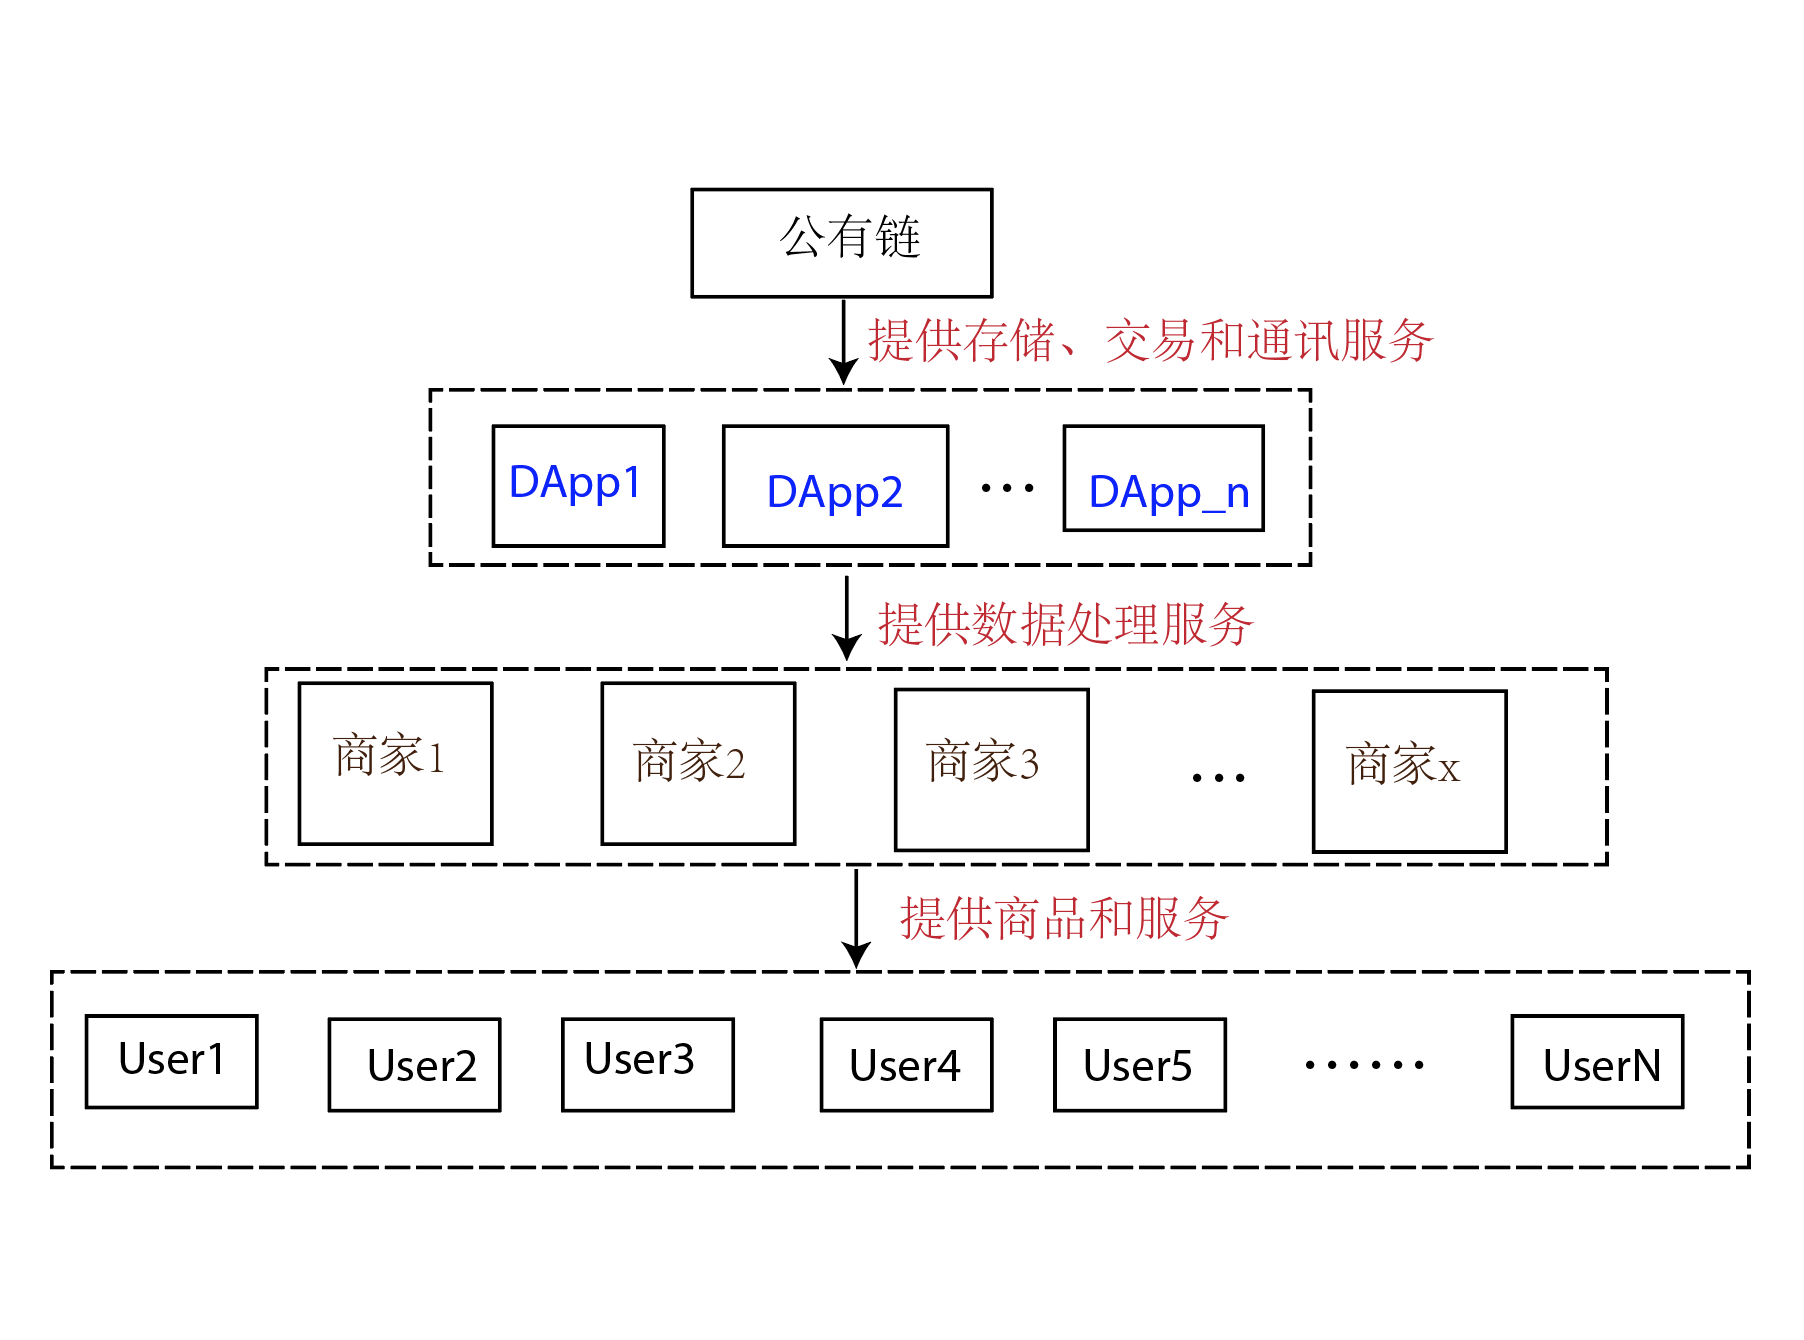
\includegraphics [width = 5in] {pic_cn/pyramid.png}
\caption {区块链生态金字塔} \label {fig: pyramid}
\end {figure}

由上图可知,CNT直接服务对象是DApp,如果把DApp主要看成开发者(D端),而D端将是人类自动化合作系统里的创业者,所以CNT主要服务对象是创业者。为此CNT主要做到以下几点:

\begin{enumerate}
\item 为开发者提供必要的功能:为此区块链需要是功能完备且无限可扩展的。
\item 减少开发者的成本:为此需要建立完善的支持,包括多语言支持、良好的文档、测试网络、大量的开源代码等。
\item 为开发者进行流量的导入:这需要用户可以共享,为此需要将用户信息放在公有链上。
\item 存储空间可以进行对象化管理:数据库的功能是各种应用最基础的功能,可读写的、基于空间的存储功能将是开发者所必需的。
\item 避免开发者形成不正当竞争:这需要数据不归结到开发者,让开发者真正提供算法服务,为此需要把数据放在公有链上。
\item 增加可以进入智能合约的交易对象:这需要区块链有跨链的功能。
\item 让智能合约足够智能:这需要智能合约拥有先知的功能。
\end{enumerate}

\subsubsection{基于空间的数据存储:可读写的存储空间}

传统互联网是建立在基于TCP协议及C/S或B/S架构上的,拥有各种垂直的应用程序。但是,由于服务器处于核心位置,而不同组织的服务器之间缺乏沟通机制,所以没办法建立跨组织的智能化、自动化的合作。区块链是建立在UDP协议支持的P2P网络上的,由于节点之间地位平等,使跨主体(包括个人和组织)的智能化和自动化的合作成为可能。传统互联网拥有完善的数据库系统,在上面可以建立大型的应用,但是,区块链系统缺乏可支持大规模应用的数据库系统,这使即使在区块链上进行跨主体的大规模合作难以建立起来。因此,CNT必须要做到的功能是链上存储的功能。另外,为了让数据生产者成为数据的控制者,需要让数据存入地址所拥有的存储空间。所以,\textbf{地址需要拥有申请数据存储空间的能力}。

从开发者的数据存储需求看,这些空间需要基于对象进行管理,而不是基于文件进行管理,以使数据在产生时进行分门另类的定义,并设计管理的方法。大量的应用都需要随时更新数据,例如通讯、社交、自媒体和网上商店等,需要后台建立可读写的存储空间。所以,可读写的、基于空间的、对象化管理的存储子链将是CNT最先需要突破的技术难题。目前看,现有的公有链都还没有实现这一功能。IPFS的项目共同特点是基于哈希进行访问,但动态的数据是以数据流形式存在,不有固定的哈希,所以基于IPFS技术的区块链的实用性是非常低的。

目前,大量针对存储的区块链项目是基于IPFS的,是基于文件进行管理的,它们将文字加密上传,公有链对其进行分片管理,其主要目的是存证,而不是面向开发者。这样基于文件的管理系统,很难实现高可用、可读写和对象化的基于存储空间的管理,也很难在上面实现数据库系统。当然,基于空间的管理需要涉及空间的贡献管理、空间的申请管理还有空间读写的管理,在分布式系统上组建这样的云服务,其复杂度可想而知,但这样基于空间分布式存储系统是区块链必须突破的难题。

在分布式云的世界里,所有的空间贡献者所贡献的空间将形成一个“世界硬盘”,对于公有链将是一个大的云空间,而申请者只是申请使用其中的部分,这就需要需要设计一套激励机制、付费机制和管理方法,使数据的读写达到高度安全和高可用。

未来的区块链基础功能应该是分布式存储,而分布式计算并不是区块链最重要的部分(虽然多次计算有校验的作用)。大量的数据只有采用分布式存储才能让个体掌握数据,并且真正实现数据在生产时就归为数据生产者所有,实现真正赋权给个人。相反,中心化的数据存储使中心化的平台占有了各种数据,不仅使他们通过数据获取利益,而且让数据处于单点风险中。在分布式云服务上建立个人文件系统,不仅让数据权归产生者,也使个人基于这一空间建议身份验证和数据交易成为可能,并且使社会的交流和交易的颗粒度更小。对于创业者,则更容易在其上建立大型的DApp,从而有可能使人类社会组织方式产生重大的变革。CNT需要开发了自己的存储子网,将空间作为管理对象,而文件作为对象管理,使每个用户在其上都可以方便的建立属于自己的数据系统、身份信誉系统、通讯系统和交易系统。

\subsubsection{基于地址的数据确权:地址处于核心地位}

区块链系统使一个地址拥有各种功能成为可能。传统世界里,当人们要进行信息交互时,需要在不同互联网平台申请账号,要进行价值交互则要申请银行帐号。在区块链上,人们有了地址不仅可以进行信息交互还可以进行价值交互。不仅如此,还可以方便地发布各种智能合约进行可编程的价值交互。另外,人们还可以将身份与地址进行绑定,辅助生物识别,建立自己的身份系统。但是在各种中心化的系统中,人们需要注册多个账号,数据也被各中心化的服务机构分割和占有,机构之间的交互难以达成,这样的合作系统既不高效也不合理,而且具有单点风险。

基于区块链的架构,我们可以设计让地址既可以作为通讯账号、社交账号、银行账号,以及个人云账号,并利用区块链的不可篡改性,让区块链数据为身份证明和信誉证明的建立提供便利。所以,只要能够实现基于地址的数据的分布式存储和通讯,所有这些功能就可以整合到一个地址里,使地址在人类交流和交易中扮演核心地位。

基于地址的数据存储和控制还使数据确权和流量共享变得极为方便。由于不同DApp的地址及与地址相关的数据都是基于地址进行数据的分布式存储,即这些数据存入用户自己的空间就可以了。这样做使用户在使用DApp时产生的数据,在产生时就可以确权,这不仅让地址的价值越来越大,也让不同DApp可以读到对方用户的数据,这使流量共享成为可能。这样做也使DApp拥有了挑战中心化平台的能力。原有的中心化平台通过“霸王条款”不断占有数据,以使自己能够主要从数据而不是服务中赚取收入,而新的DApp在CNT上开发时原有的DApp都可以为其提供流量,而新的DApp也可以为原有的DApp带去流量。关于DApp的数据共享如下图所示:



\begin {figure} [htbp]
\centering 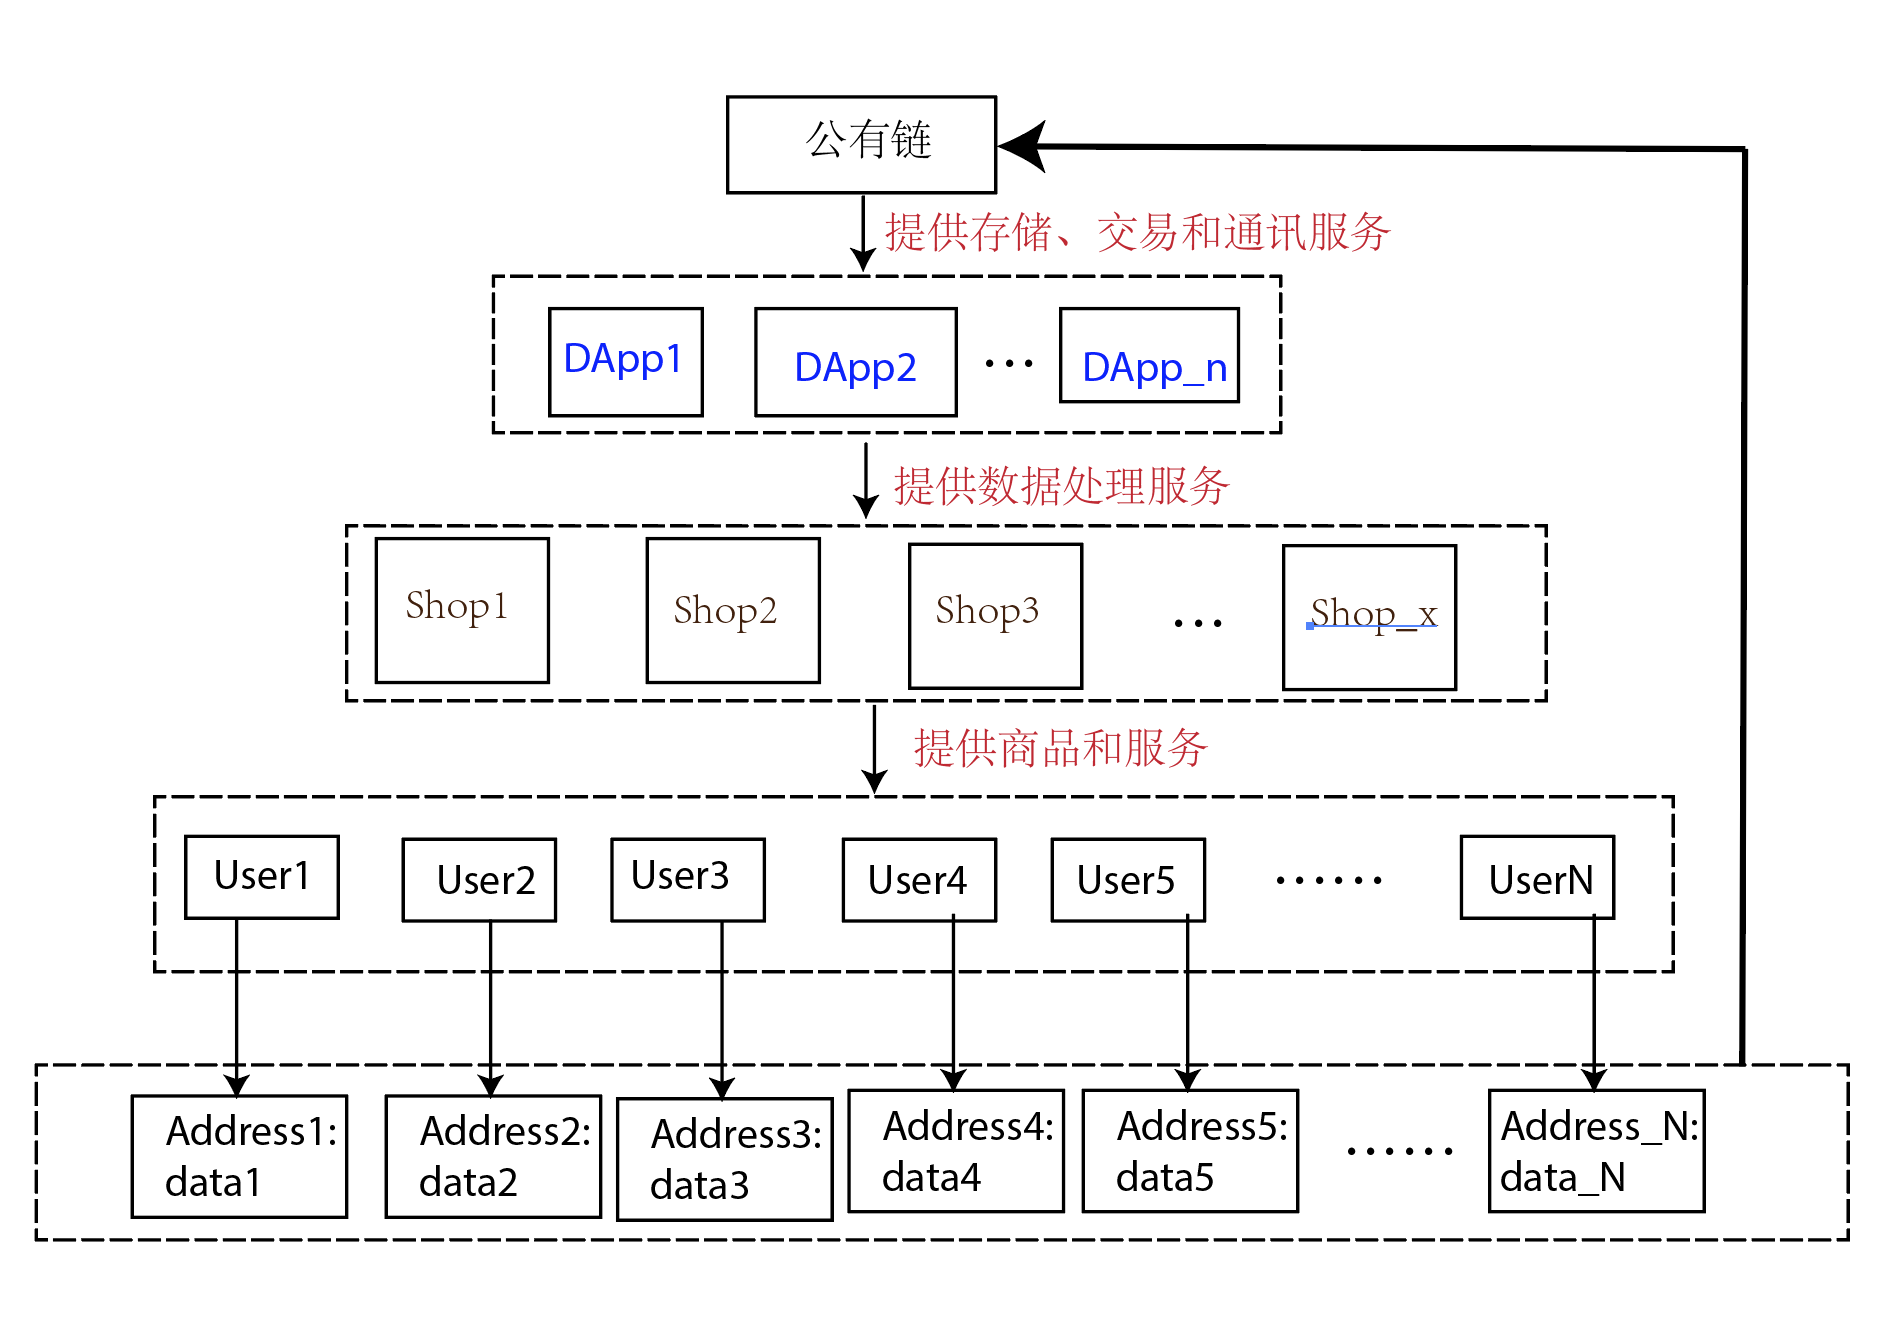
\includegraphics [width = 5in] {pic_cn/address and data.png}
\caption {DApp流量和数据共享} \label {fig: address_and_data}
\end {figure}

CNT在实现分布式数据存储的基础上,使任何DApp都有能力赋予地址数据存储、信息交流、价值交互和身份证明等的能力,使任何个人、组织甚至智能程序,只要有拥有一个地址就可以方便地与任何其他任何主体建立交流和交易关系。不仅如此,随着以地址为核心的数据的积累,还可以建立一个“良币驱逐劣币”的信誉证明系统,使人类合作走向良性循环。

从交流和交易的主体看,只要拥有操作地址的能力,任何主体都可以参与CNT系统进行交流与交易,它们可能是个人、组织或智能程序。当前的世界是各种中心化组织主导的世界,区块链正使个人崛起,而在未来智能程序将成为越来越重要的主体,但是其实不必区分地址后面是人还是智能程序,是个人还是组织,只要申请并拥有地址就可以实现这些主体之间平等交流和交易。

根据梅特卡夫定律,越多主体参加到一个系统中将越能促进系统进步。参与者,不管是个人、企业还是智能程序,通过底层的区块链代码,他们可以不受地理、制度和组织的限制,自由表达观点、出售产品和购买产品,并通过智能合约让交易更加自动化和智能化,从而使人类逐步建立大规模的、自动化的深度合作关系。

\subsubsection{基于数据路由的数据分享:信息交流得到协议全方位的支持}

CNT的存储功能使数据可以链上存储,而数据获取时需要进行数据路由。CNT设计专门的数据路由功能,让数据随时可以访问,也使任何地址之间建立信息交流。为了能够达成畅通的聊天的体验,现在的方案都需要中心化的存储或路由。CNT的分布式存储针对聊天进行了专门的优化,使用专门设计可读写的存储空间和文件数据库可以实现聊天不通过中心化服务器就可以完成。

信息交流,不论是两人会话还是多人会话,不论是文字、语音还是视频,对于人类交易在事前、事中和事后都是异常重要的。信息互联网的特点是信息交互,而价值互联网的特点是价值交互,但作为新一代公有链的CNT将打破这种界限,将信息交互与价值交互融为一体。

CNT为DApp提供协议级的通信支持,使所有人通过地址就可以与全世界进行加密的、去中心的自由交流。交流数据将仅由生产者拥有。任何人都可以建立点对点的富媒体聊天,多人组群聊天,并且在交流中就可以进行转账和智能合约交互。通讯功能整合到区块链是很重要的:在交易前,可以联系对方进行交易的协商,并在会话中就可以方便的建立交易的智能合约;在交易中,双方随时可以对交易相关情况建立聊天,沟通交货情况或修改智能合约;在交易后,所有曾经交易过的对象都可以分门另类的建立群组,可以方便地进行客户关系管理。

CNT将在协议层为分即时聊天,即Email,加以支持,而DApp基于Email和分布式存储功能,可以实现建立点对点或一点对多点的关系,并进行点对点或群组聊天。

\subsubsection{系统是完全分布式和无限可扩展的}

Contatract是完全分布式的。CNT类似比特币和以太坊,并不需要任何超级节点的选举,任何人都可以参与挖矿,并且有机会获得挖矿奖励。参与者可以选择获得参与共识主链或申请参与到功能子链的各分片提供资源。

不管是Windows系统、平果系统还是安卓系统,通过CNT软件就可以共享磁盘或参与挖矿,从而极大的扩大了分布式和可扩展性。

Contatract是无限可扩展的。所谓无限可扩展,是指区块链系统能够随着矿工的增加其能力得到不断扩展并能支撑更多的用户。CNT将采用分片机制的,所以随着参与矿工数量的增加,各功能将得到不断的扩展。

\subsection{基于地址的数据系统}

\subsubsection{基于个人云空间的身份验证、朋友圈和交易记录的信誉证明}

人与人的交流与交易离不开信誉机制。因为人们的交流和交易常常需要知道交流和交易的对象是怎样的人,从而可以使信息更加对称,以便高效地达成交易。对于良好运作的市场,信誉是“良币驱逐劣币”的最重要的机制。区块链应该为信誉机制提供接口,使人们的信誉能够随时间动态变化,并促进地址拥有人维护自己的信誉。

信誉实际上是关于该地址拥有者的信息(包括身份信息)的评价,为此应该把尽可能多的信息整合到地址,而CNT是以地址为核心进行数据存储的,很容易通过多种信息实现信誉证明(proof of reputation,PoR)。人们可以通过自愿信息披露,将与世界发生关系进行记录,也可以采取第三方身份验证的机制来建立自己的信誉。不同的方式证明效力有别,CNT提出弱式证明、半强式证明和强式证明三种证明途径:

\begin{enumerate}
\item 弱式证明:通过自己发布信息,让虚拟世界与现实世界不断建立联系,通过在时间轴上不断沉淀的自己生活的动态信息来证明自己,这主要是通过社交功能来实现。
\item 半强式证明:通过与其它地址发生交易,并提供交易相关信息(包括交易方的点评)来证明自己。
\item 强式证明:将自己的地址相关信息与现实世界建立可信的关联以证明自己。该方式主要是通过可信的渠道公布自己与地址的关系来实现或者通过第三方验证来实现。比如,一家机构通过在自己的官网公布自己的区块链地址,或一个人到专门的验证机构验证,由验证机构在自己的信息发布渠道公布该地址对应的真实的人的身份。与此同时,地址拥有者可以在自己的地址上发布相关验证信息,以方便向其他可信主体求证。
\end{enumerate}

为了完成信誉证明,个人可以选择将个人信息、生活动态数据库和交易数据保存在自己的空间,并针对性授权给不同的人使用。
未来可能有越来越多的人将数据沉淀以地址为标识的私有数据里,比如:

\begin{enumerate}[itemindent=1em]
\item 通讯录数据:赋予地址对通讯录进行权限管理,其中有一种权限是授权给相关人员帮助将地址中的数据转移到新地址,这在类似丢失私钥等紧急情况下可以使用;
\item 生活动态数据:赋予地址发布不可篡改的生活动态的能力;
\item 多媒体数据:赋予地址发布文本、图片、语音、视频等媒体的能力,并且赋予地址自定义标签和自定义可篡改属性的能力;
\item 产品数据:赋予地址发布各种产品,包括可以共享的资源的能力,并将这些数据存放在产品数据库;
\item 文件存储空间:赋予地址申请空间及保存各种数据的能力,由于文件是以对象形式存在,地址可以定义自己的数据库,这为建立各种DApp的数据库铺平了道路;
\item 多币种钱包数据:赋予地址把各种代币通过跨链交易映射到链上的能力形成自己的多币种钱包数据库;
\item 链上发币数据:赋予地址一键发币的能力并将相关数据保存在发币数据库;
\item 智能合约数据:赋予地址生成智能合约的能力,并把相关信息保存在智能合约数据库。
\end{enumerate}

由于数据产生后就储存在私有数据集里,这就解决了数据隐私保护和确权的问题,也为数据交易铺平了道路。只有地址愿意开放的数据才会被公开,地址还可以选择性的将数据开放给指定的地址,并形成自己的数据分享圈子,比如生活动态数据只有指定的朋友能看到。这些分享还可以设定访问的时间限制或有偿查看,从而形成各种类型的数据交流和交易。

未来可能出现专门的数据二道贩子,不断从个人手里收购各种脱敏数据,从而让数据真正成为一个服务业。

\subsubsection{地址别名、通讯账号和帮助恢复功能}

CNT提供的主要功能是面向用户通讯和交流,而用户通讯交流需要给用户绑定记忆友好的ID, 而不是枯燥乏味的二进制地址串。所以CNT提供地址别名作为更友好的界面。

由于通讯需要对方公钥加密,所以地址还将可以申请专门的通讯账号并将通讯账号可在于世界状态,以便用于数据的加密通讯。

拥有私钥就拥有一切,但丢失私钥就丢失了一切,为避免这种悲剧,CNT将设计地址可以指定其它地址加入多重签名,从而实现丢失私钥时,在一定期限后其它地址的私钥可以帮助授权将数据或账户余额转移到其它地址的能力。

\subsection{设计目标}

虽然近年来区块链被认为有颠覆性现有商业模式的潜力,但是,区块链公链的底层技术还不足以支持大规模的商业应用,区块链目前最突出的技术问题就是系统性能低下。以以太坊为例,其全网所有运行的应用,可以使用的处理能力约每秒10笔左右,但是针对一款日活千万级别的应用,其TPS峰值要求一般在2000-3000左右,所以现有的以比特币和以太坊为代表的区块链1.0和区块链2.0系统,完全无法支持大规模的商业应用。

而TPS这个限制为什么这么难以突破呢?正如同所有分布式系统在设计时都会面临的“不可能三角”问题一样,区块链系统也会面临自己的不可能三角:去中心化、安全和高性能。

1. 去中心化的设计挑战,是如何保障网络的去中心性,这就要求该网络需要是一个对等网络,该网络中的机器的地位都是平等的,不存在任何特殊化的中心节点,同时为了保证该网络的去中心性,该网络需要是一个开放的无准入的网络,从而可以让人人都能够加入该网络,且该网络不会被一个或多个中心控制;

2. 安全的设计挑战,是保障该网络足够安全,难以被人破坏。在一个开放并与经济利益挂钩的网络中,不仅会有好人购买机器加入这个网络,也会有更多的坏人企图希望通过破坏该网络获利。那么,如何在网络内部存在坏人的情况下,保证网络的安全性,这已经突破了传统意义上的安全架构,是安全设计的挑战;

3. 高性能的设计挑战,则在于尽可能的保证网络足够去中心和安全的情况下,能够保障的性能最优以及网络能耗最低。

在区块链不可能三角中,比特币和以太坊选择了足够的去中心化和安全,而EOS偏向了效率,牺牲了一部分去中心化和安全。

CNT的目标是以区块链技术构建交流与交易的平台,在这个平台上数据资产、多种代币、商品与服务可以通过智能合约自由交互,在很好的平衡不可能三角的三支角的情况下,实现价值互通。具体而言,包括下列技术需求:

(1)系统功能
\begin{itemize}[itemindent=1em]
        \item 具有无限可扩展的交易和图灵完备的智能合约的功能。
        \item 具有方便的数据保存的功能。
	\item 具有方便的异步通讯的功能。
\end{itemize}

(2)系统特性
\begin{itemize}[itemindent=1em]
	\item 系统稳定与高并发。
        \item 分布式应用程序容易开发和布署。
	\item 能够尽量模块化,以方便系统升级和维护。
\end{itemize}

(3)可扩展性
\begin{itemize}[itemindent=1em]
	\item 能够满足大规模交流与交易应用的需求。
	\item 能够在系统达到大规模的情况下保持合理的能效比。
	\item 能够在系统自身规模和应用规模扩张的情况下,出块效率、存储效率、通讯效果能够保持良好。
        \item 随着越多的资源的加入,可以让系统达到无限可扩展。
\end{itemize}


(4)安全性
\begin{itemize}[itemindent=1em]
	\item 能够防止双花攻击。
	\item 能够防止女巫攻击。
        \item 能够防止其它降低效率或系统瘫痪的攻击。
\end{itemize}


\subsection{系统架构}

基于以上的分析,系统至少要拥有一个存储子网,分片交易子链,协调分片的主链,在各分片上运行的智能合约和以地址为中心的用户支持系统。下图可以概括这一功能完备的区块链的主要架构。

\begin {figure} [htbp]
\centering 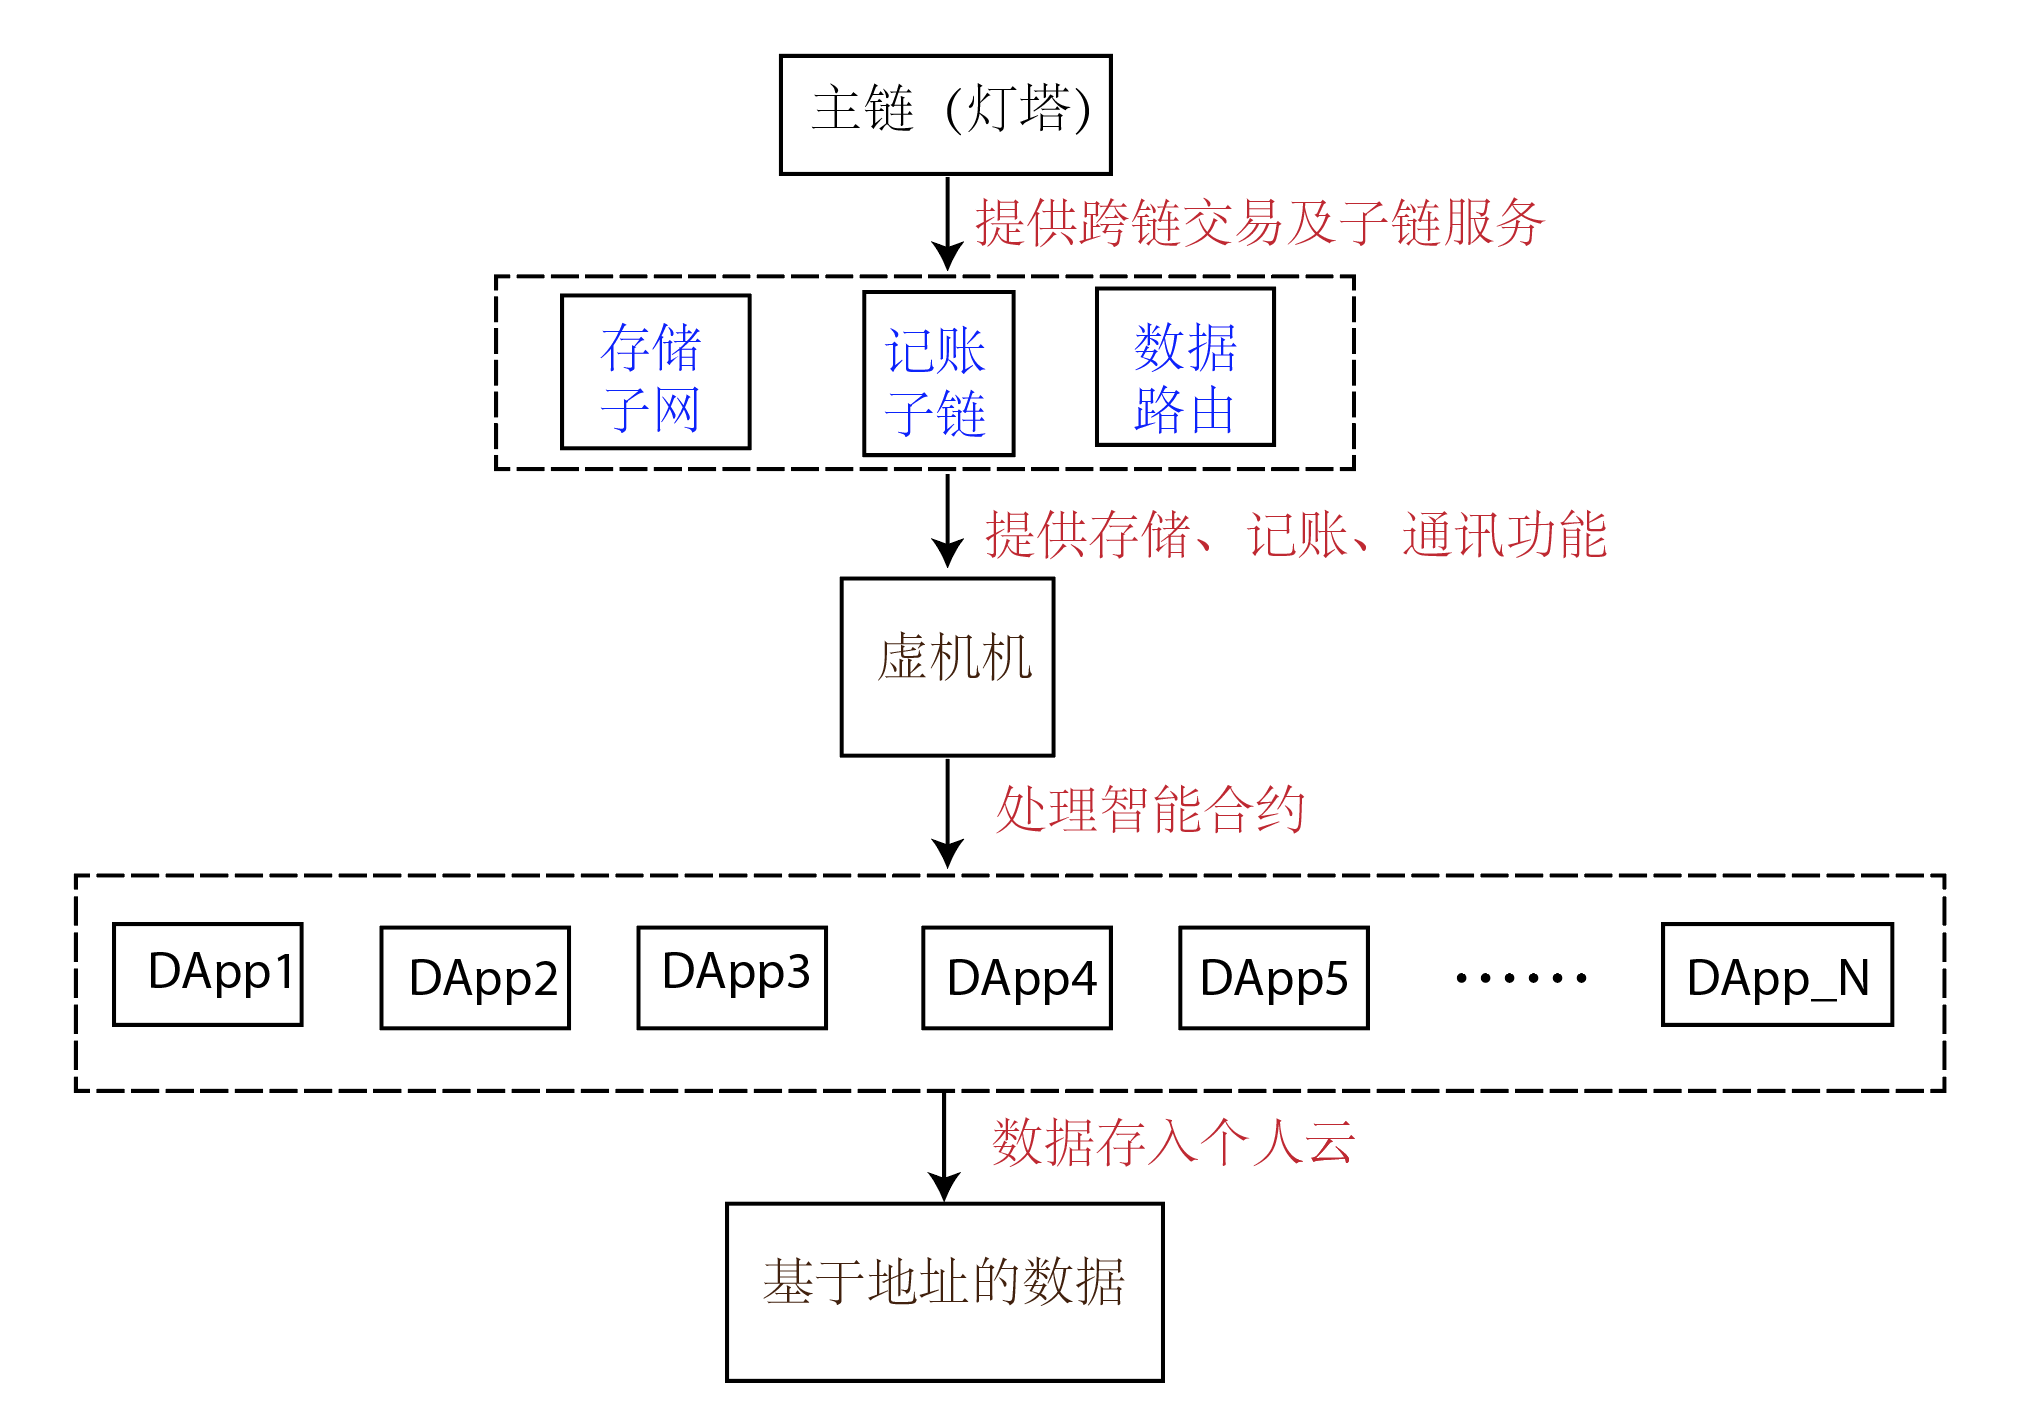
\includegraphics [width = 5in] {pic_cn/framework_cnt.png}
\caption {系统架构} \label {fig: structure}
\end {figure}

以下各章,在技术方面,将主要讨论如何实现基于空间的存储、如何实现分片以及如何实现基于个人云的通讯等三个方面的问题。而经济模型方面将讨论代币经济模型和项目未来计划。

\section{基于空间的存储}
\subsection{基于对等网络的存储}
\subsubsection{存储链的架构}

传统区块链,大多属于状态区块链(Status BlockChain),从比特币的bitcoin数量这一单一状态,再到ethereum的智能合约世界状态。无不遵循着状态存储的逻辑。

从IPFS开始,出现了数据区块链(Data BlockChain),数据区块链是将数据的属性当作状态来进行交易和存储,从存储角度来说,IPFS实现了对象存储,它的对象就是文件。提出了两种矿工,一种作为存储矿工,以保存文件数据为己任;一种是索引矿工,主要用来保存文件描述信息(文件属主,分片数量,分片hash等等属性)

CNT提出的概念并不是对象存储,而是一种纯粹的空间存储,它不针对具体的存储对象,而是提供可用的存储空间。用户可以像使用本地硬盘一样使用该存储空间,将之用于存储各种数据对象,而这个空间是分布式矿工节点提供的。

下图是CNT的存储子网的架构:

\renewcommand\figurename{图}

\begin {figure} [htbp]
\centering 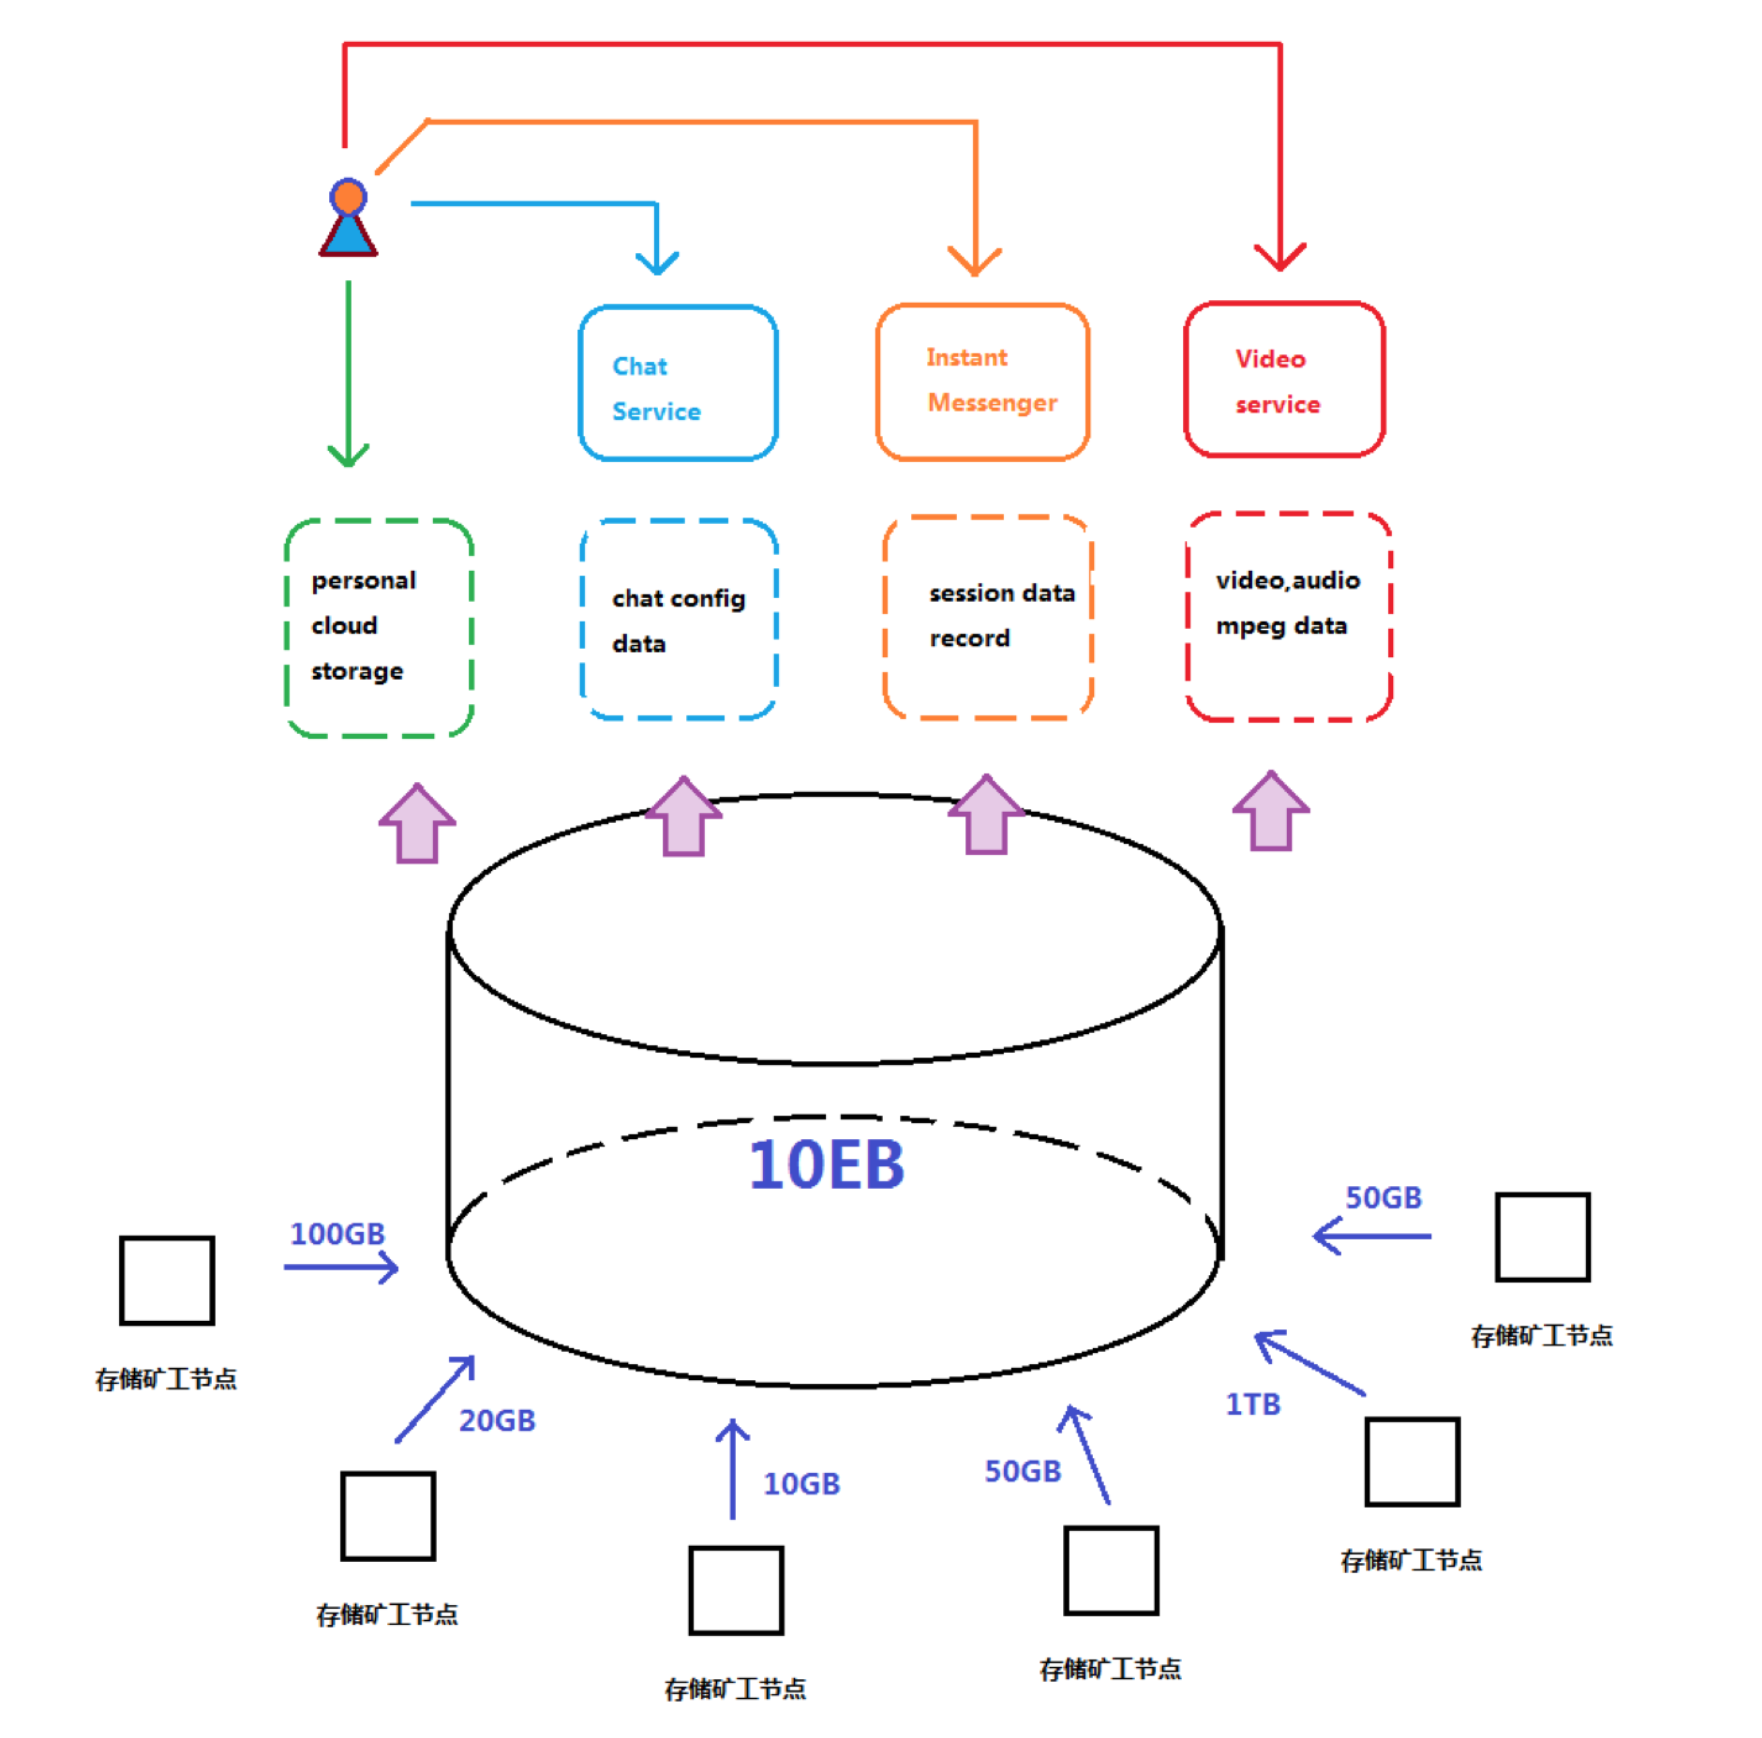
\includegraphics [width = 4.5in] {pic_cn/storage.png}
\caption {CNT存储功能} \label {fig: storage}
\end {figure}

如上图所示,存储贡献者(存储矿工)提供自己主机或者节点的空闲存储资源,CNT将矿工们的资源进行聚合,形成大规模的存储云。

有了超大容量存储云,钱包(终端)用户就能够从云中将一段虚拟存储空间(比如1GB)提取出来形成自己的云盘,用户可以自己规划往空间中存储文件,可以保存大体积的文件,比如音视频数据,也能保存大量的小文件。这些文件或者数据的上传下载,寻址,使用,管理维护等都由用户自己在虚拟云磁盘中规划,无需像IPFS那样去执行复杂的市场交易,来完成少量文件的存储。

另外,有了分布式存储云,我们可以在其上构造功能更加复杂的分布式服务,比如聊天室、即时通讯、音视频服务等等。这些传统的中心化服务在解决了存储痛点之后,都有机会实现去中心化。

而存储矿工们的主要任务就是保持和维护好自己提供的物理空间和映射管理的虚拟空间,让它们持续在线提供服务就可以不断地获取挖矿收益。

存储子链的角色如下图所示:

\begin {figure} [htbp]
\centering 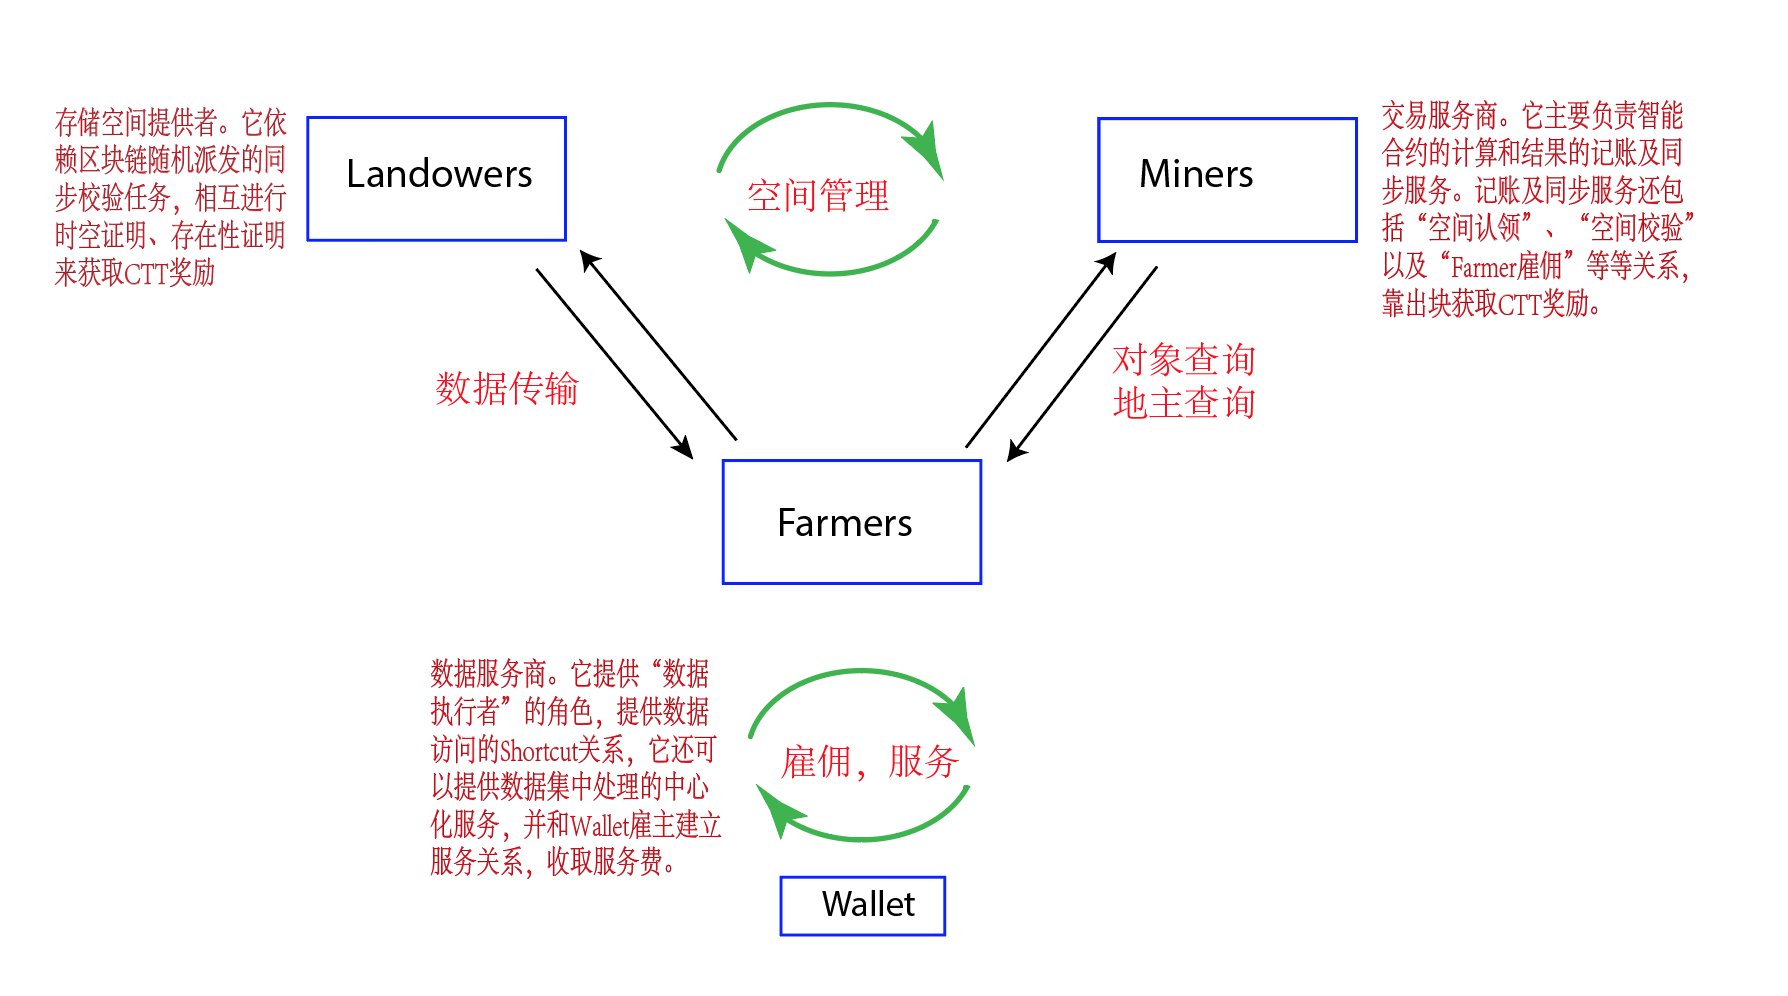
\includegraphics [width = 5in] {pic_cn/framework_storage.png}
\caption {存储子链的角色} \label {fig: d0}
\end {figure}

从上图中我们看到四个角色,Wallet表示前端,Farmers表示存储空间服务提供者(也可以被称为地主,即landowner),Miners表示区块链服务提供者,其中还有一个重要的角色是“Data Gateway”,又被称为数据代理(Data agent),提供数据路由的功能。

\subsubsection{数据代理}

如果没有数据代理,当用户要写入数据时,需要走一段复杂的网络路径以建立信息查询,才能开始传输。这无疑将为使用体验带来了很严峻的考验。为了使用户走捷径(Shortcut),就需要代理帮助事先完成,未来每次访问都轻车熟路。代理将该用户经常访问的数据对象做好各种信息查询和路径的准备,等到用户提出请求时,所需要等待的时间将会大大缩短,体验能大大提升。以Email服务举例,代理可以提供属于用户的邮件列表空间的读写,从而大大加快邮件的传递速度。

所以,用户与代理之间就构成了一个“中心化”的私人雇佣服务,相当于用户能够通过交易(花费CNT币)在网络上寻找一个为他提供专属数据服务的数据服务商。该服务商主要负责雇主的数据访问的路径建设、传输和简单的列表管理等业务。

\subsubsection{存储矿工挖矿}


\begin {figure} [htbp]
\centering 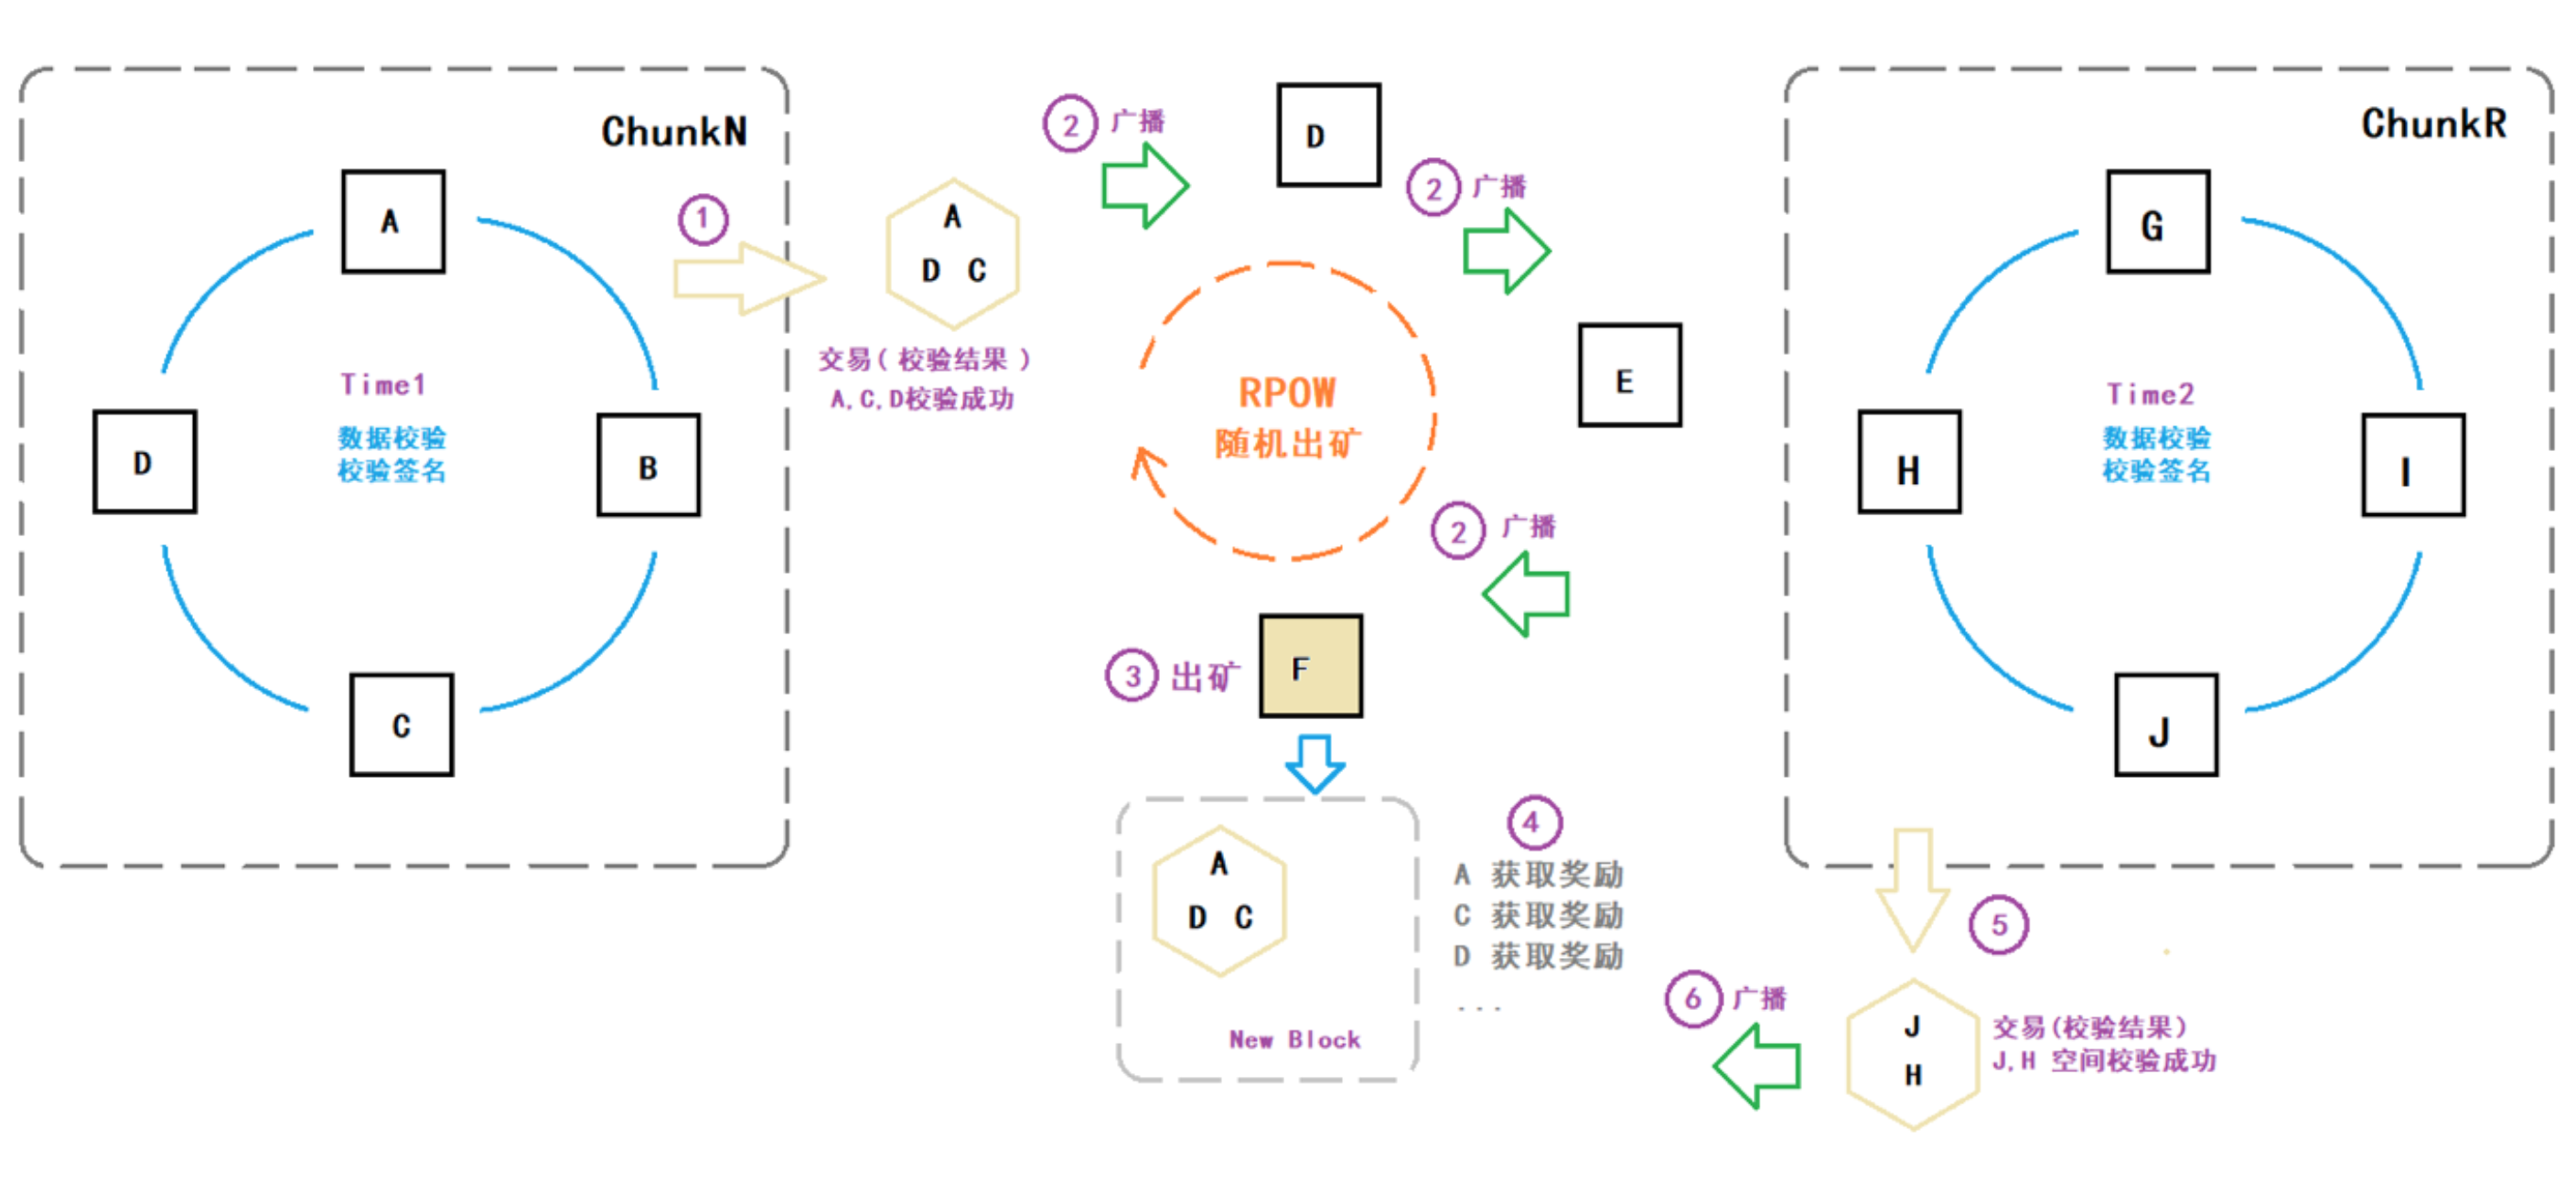
\includegraphics [width = 5in] {pic_cn/storage_mining.png}
\caption {存储矿工挖矿示意图} \label {fig: d2}
\end {figure}

CNT将虚拟存储空间都划分为Chunk,存储矿工在确定提供一定量的存储后,就能够认领自己提供空间的Chunk,比如A矿工确定提供1GB,它被算法分配到了ChunkN(比如ChunkN为虚拟空间的3GB~4GB范围)。认领同一个Chunk的矿工彼此形成数据副本,我们称为副本组(Chunk Copy Group), 如上图认领不同虚拟空间的存储节点A,B,C,D和G,H,I,J形成了ChunkN和ChunkR 的两个副本组。

在Time1时间由ChunkN的副本组的四个节点ABCD互相验证数据,它们彼此提供跟自己Id和当前区块hash关联的Chunk片内数据偏移和数据尺寸计算hash,将hash交给其他节点进行验证,验证通过即签名并继续传递,不通过即丢弃。当签名数达到2/3节点时即可认为认证通过。
图中,ChunkN中有A,C,D三个节点通过彼此的数据校验,并成功签名。于是将这份签名打包成一笔“空间校验交易”。将这笔交易在所有矿工节点之间广播传递。

最终“空间校验交易”由RPOW确定的矿工进行新区块打包,新区块将这笔校验交易打包到区块中,再进行全网广播。收到新区块的节点根据区块中的空间校验交易中包含的A,C,D三个存储节点关联的账户进行token奖励。于是维持存储空间在线就能产生收益了。


\begin {figure} [htbp]
\centering 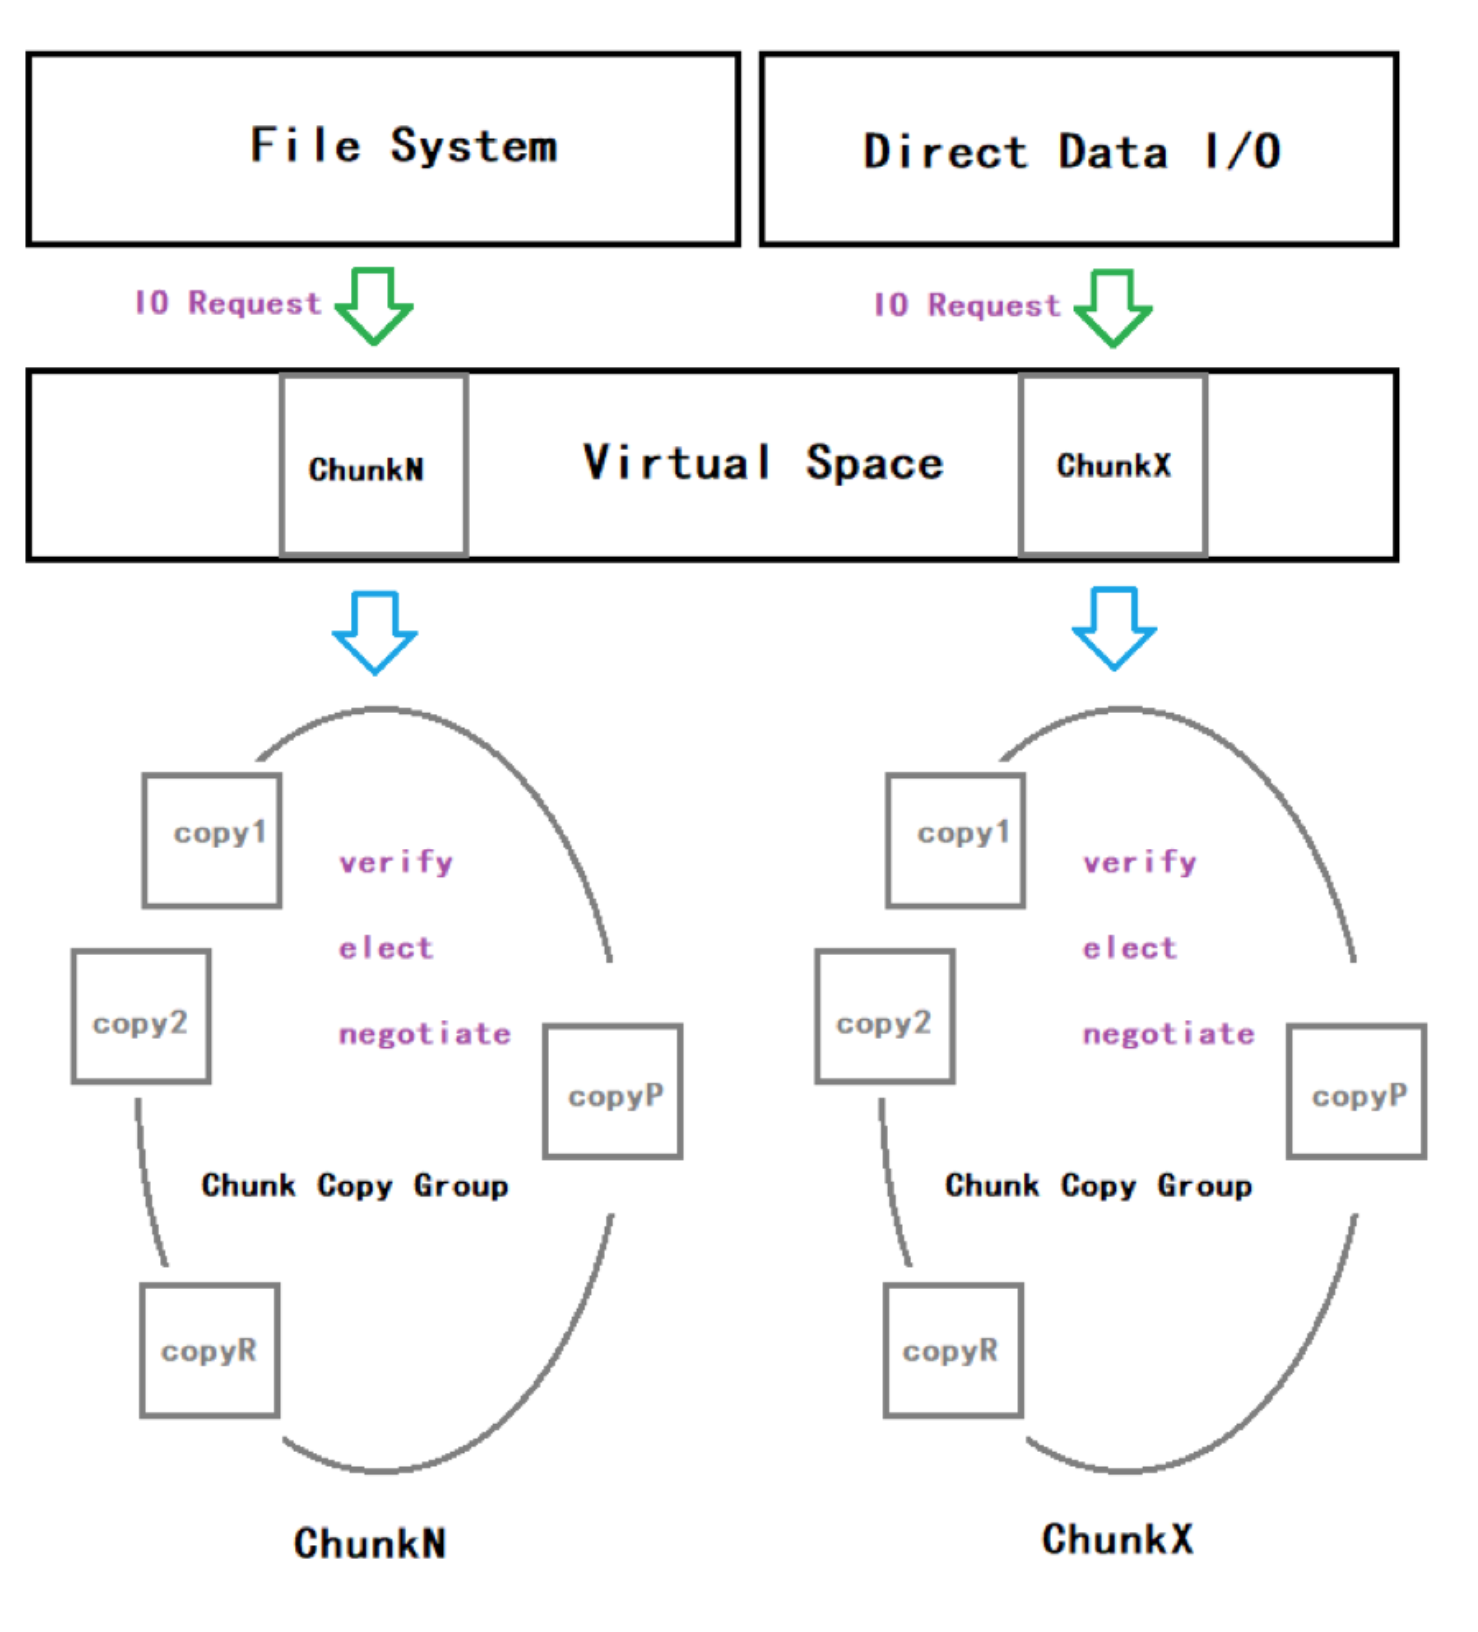
\includegraphics [width = 5in] {pic_cn/storage_verify.png}
\caption {存储矿工验证示意图} \label {fig: d3}
\end {figure}

\subsubsection{分片与加密}

存储分片采用空间分片的模式,跟现今大部分公链的文件分片不同:

传统来说将文件分割为数个等长片段在网络上分布存放,下载读取时并行读取到本地拼接,这种方式的优势在于实现简单直接,将文件片段内容hash进行merkle整合,来保障文件数据的一致性下载的多片段同时下载也让读取速度提升不少;但它的缺点也相对明显,因为大文件的分片数量庞大,维护相对困难;而文件尺寸固定,让它的存储模式仅仅局限在只读上,一般不支持文件修改,只能适用于归档场景。从功能角度描述相当于网络文件存储,跟传统的P2P文件模式一致,对标中心化服务,就是跟FTP类似。

CNT不针对文件,而是提出一个存储空间访问的途径,存储链矿工通过共享磁盘中的空闲存储空间,来获取token。跟IPFS和其他存储类产品思路不同的是,这里不管是否有文件上传使用,空间都能够给矿工带来价值,网络上无数的存储共同构建一块超大的虚拟磁盘,CNT将磁盘总量按照一定容量划分成空间切片Chunk集合,将链上存储矿工的资源跟Chunk关联绑定,形成一个巨大的存储池。为什么是提供存储池,有了这个分布式虚拟云存储池,用户就能够从中分配自己想要的空间,就能够自由对其中的文件或者数据进行随机读写,从这个角度来说,它对于用户来说更像是一个云存储设备,而不是一个FTP服务器。这种链内的块存储设备(Block Device)上,我们在存储终端构造一个简单File System就可以用来存储


\begin {figure} [htbp]
\centering 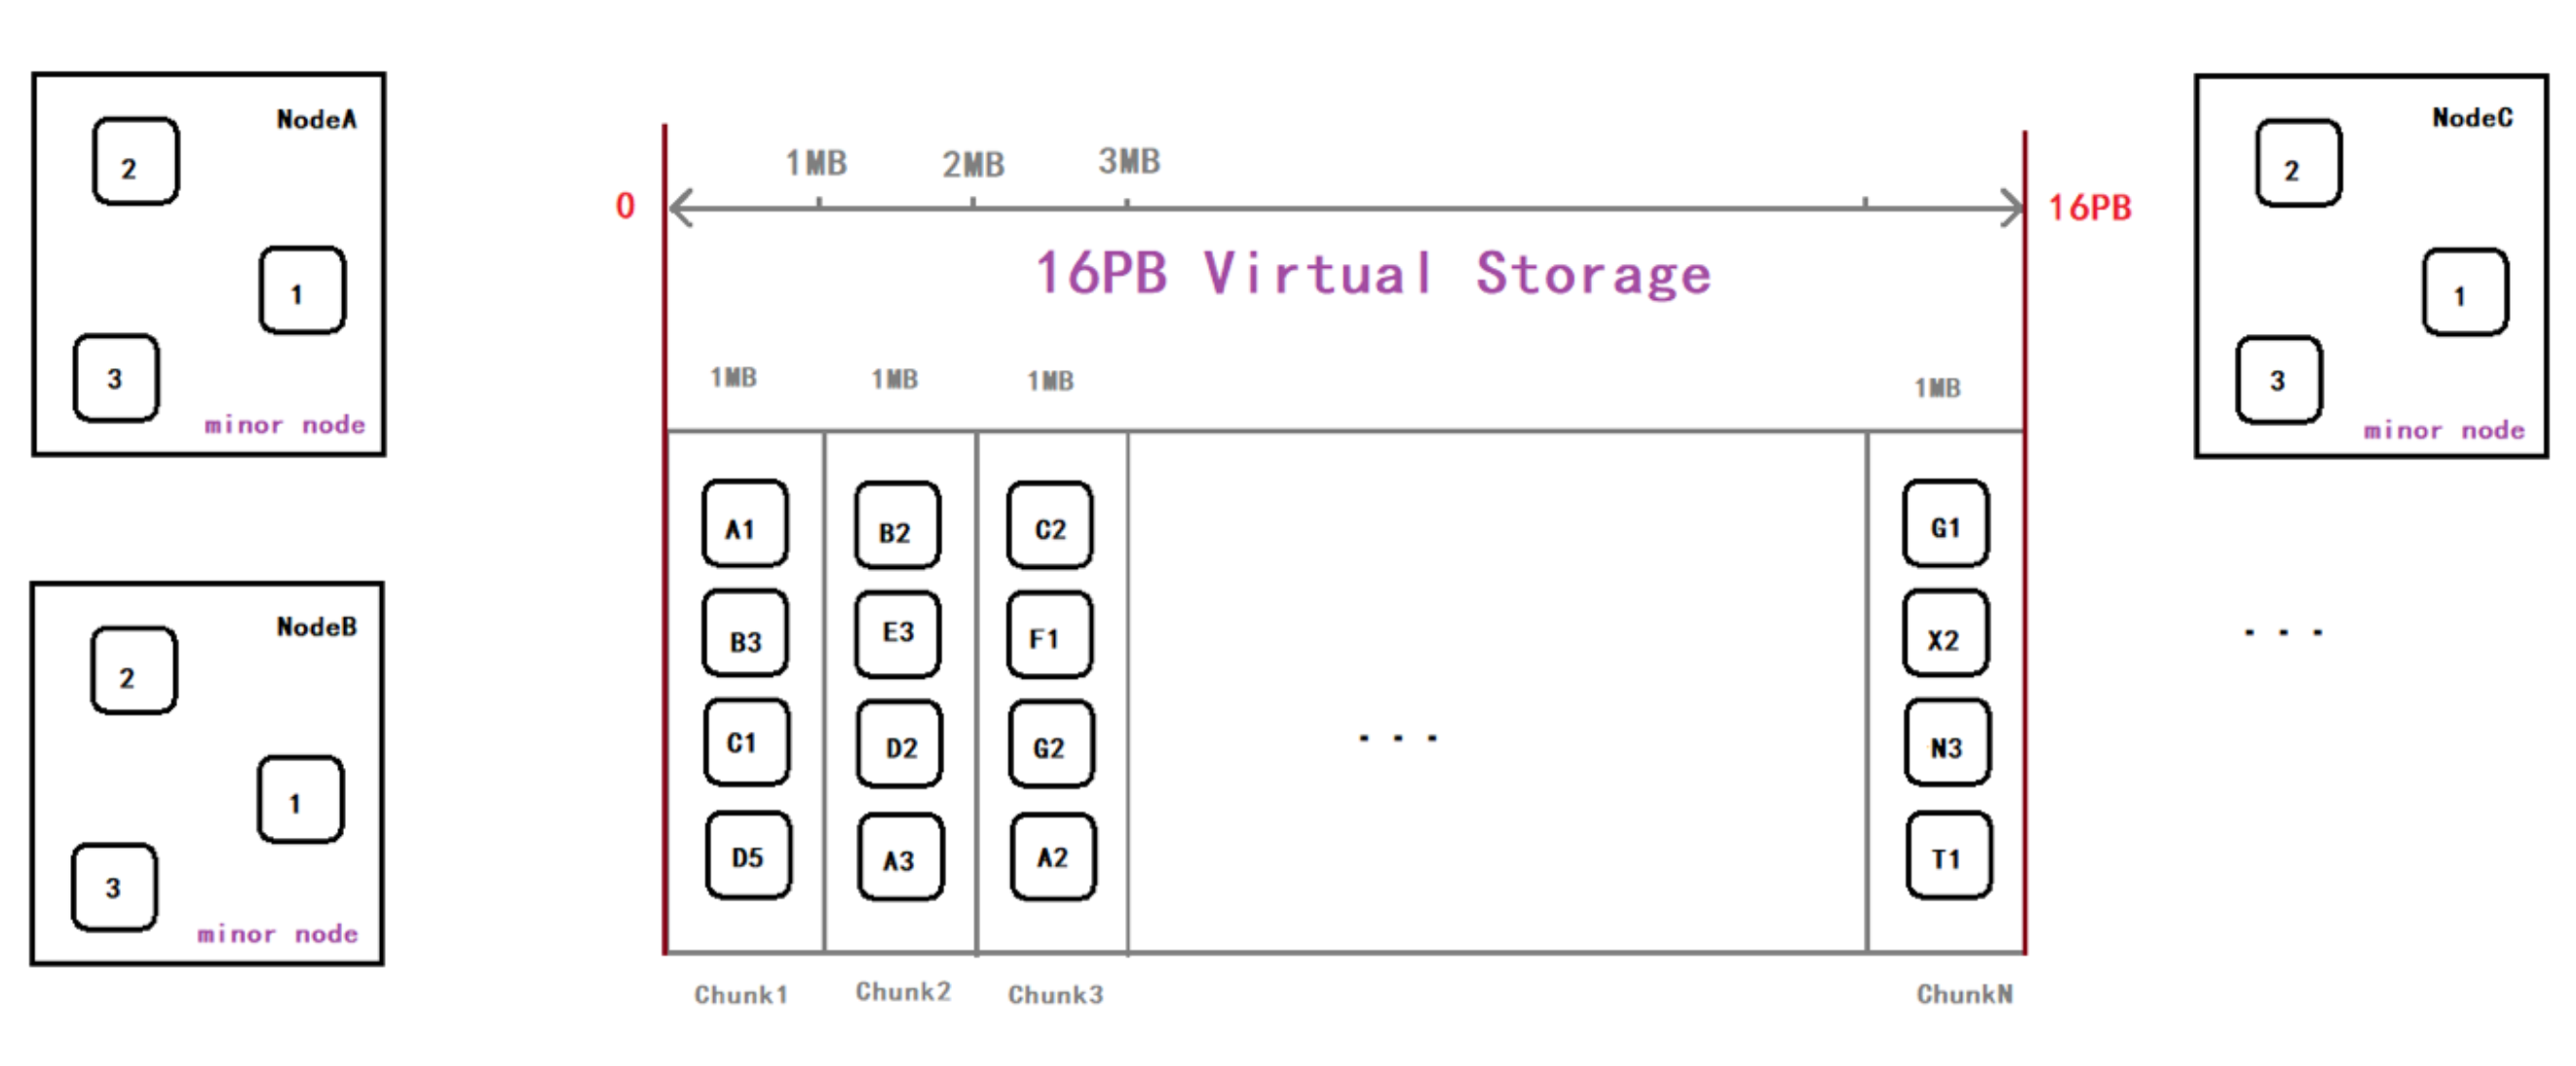
\includegraphics [width = 5in] {pic_cn/chunk.png}
\caption {分片与加密} \label {fig: d4}
\end {figure}

如上图所示,16PB虚拟空间中包含有很多Chunk, 每个Chunk是一个固定容量(比如1MB大小),对于存储矿工节点而言,它们贡献空间的方式就是贡献块副本,图中每个Chunk都由多个矿工贡献的块副本构成,所以Chunk是一个逻辑概念,它代表的是虚拟空间中的一段,比如Chunk1 表示虚拟空间中的0-1MB这段空间,而Chunk2则表示虚拟空间中的1MB-2MB的空间…;每个Chunk都可以由多个矿工提供的1MB块来构造,副本数量可伸缩,根据不同阈值来做不同的认领策略。

\subsubsection{矿工分组}

存储矿工分组涉及两个层面:

1.	采用Chunk方式的管理,将所有参与维护同一数据的节点集合到一起,成为一个Chunk维护组

2.	为了保证数据的高可用,Chunk空间副本数量比较多,也就意味着Chunk的管理信息也需要占用比较庞大的管理空间(内存和存储)。


\begin {figure} [htbp]
\centering 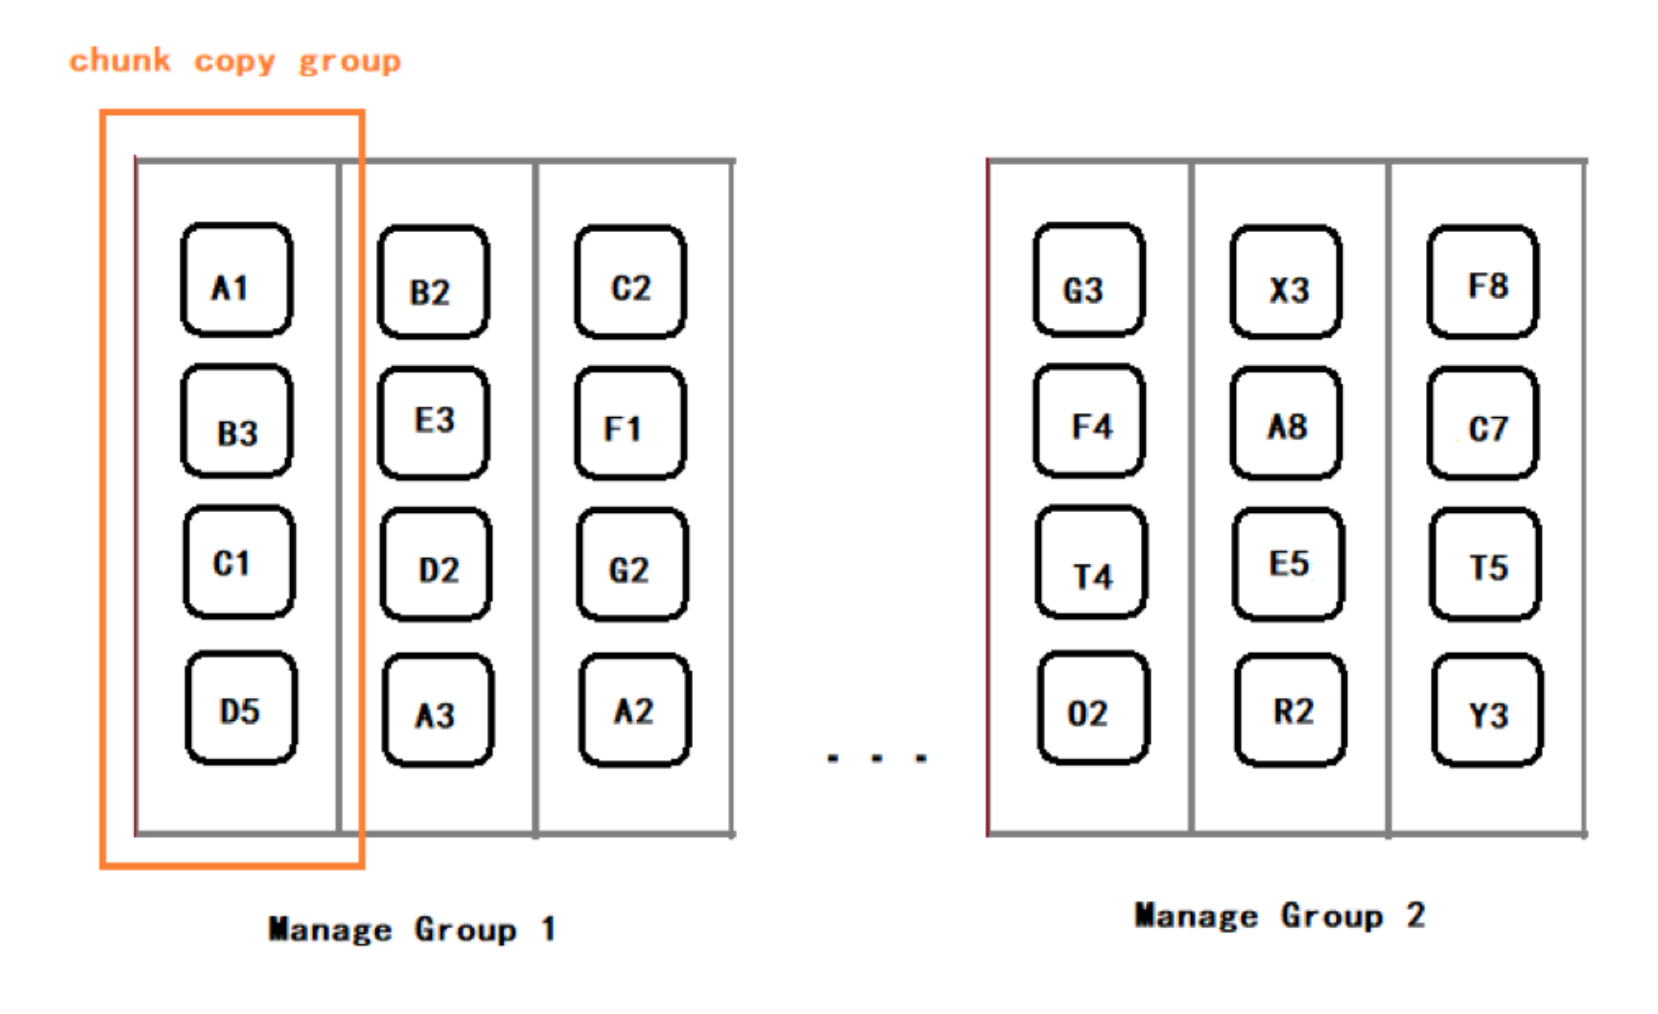
\includegraphics [width = 5in] {pic_cn/chunk_group.png}
\caption {分片与加密} \label {fig: d5}
\end {figure}

对于同一个矿工节点,它是各个chunk的空间载体提供者,它参与到所有它认领(提供空间)的Chunk copy Group 中,在这个Group中,跟其他参与同一个Chunk的节点进行数据同步,共同维护同一个Chunk的高可用

而对于每个Chunk, 需要记录它们的副本参与节点的情况,CNT根据ChunkId和矿工节点的NodeId的对应关系,将所有的Chunk分成若干个Manage Group,分别交给一组矿工节点进行信息记录和管理。这就使得矿工对Chunk形成了管理分片,就形成了存储区块链的分片机制。

区块链的分片机制,是为了提升区块链整体运行效率,使得更多的信息和交易得以并行处理。


\subsubsection{数据下载}

数据下载,用户节点根据数据请求(来自File System,或者上层直接数据访问)向一组Chunk请求数据。

对于同一个Chunk Copy Group内的所有节点,请求节点发送命令索取大家当前更新区块的Id和当前状态, 索取成功后,将Id最大并且相等,状态为“status online”的几个节点归为数据提供节点,根据向该Chunk请求数据大小,将下载请求切分为不同的片段请求。同时向它们发起数据传输连接。


\begin {figure} [htbp]
\centering 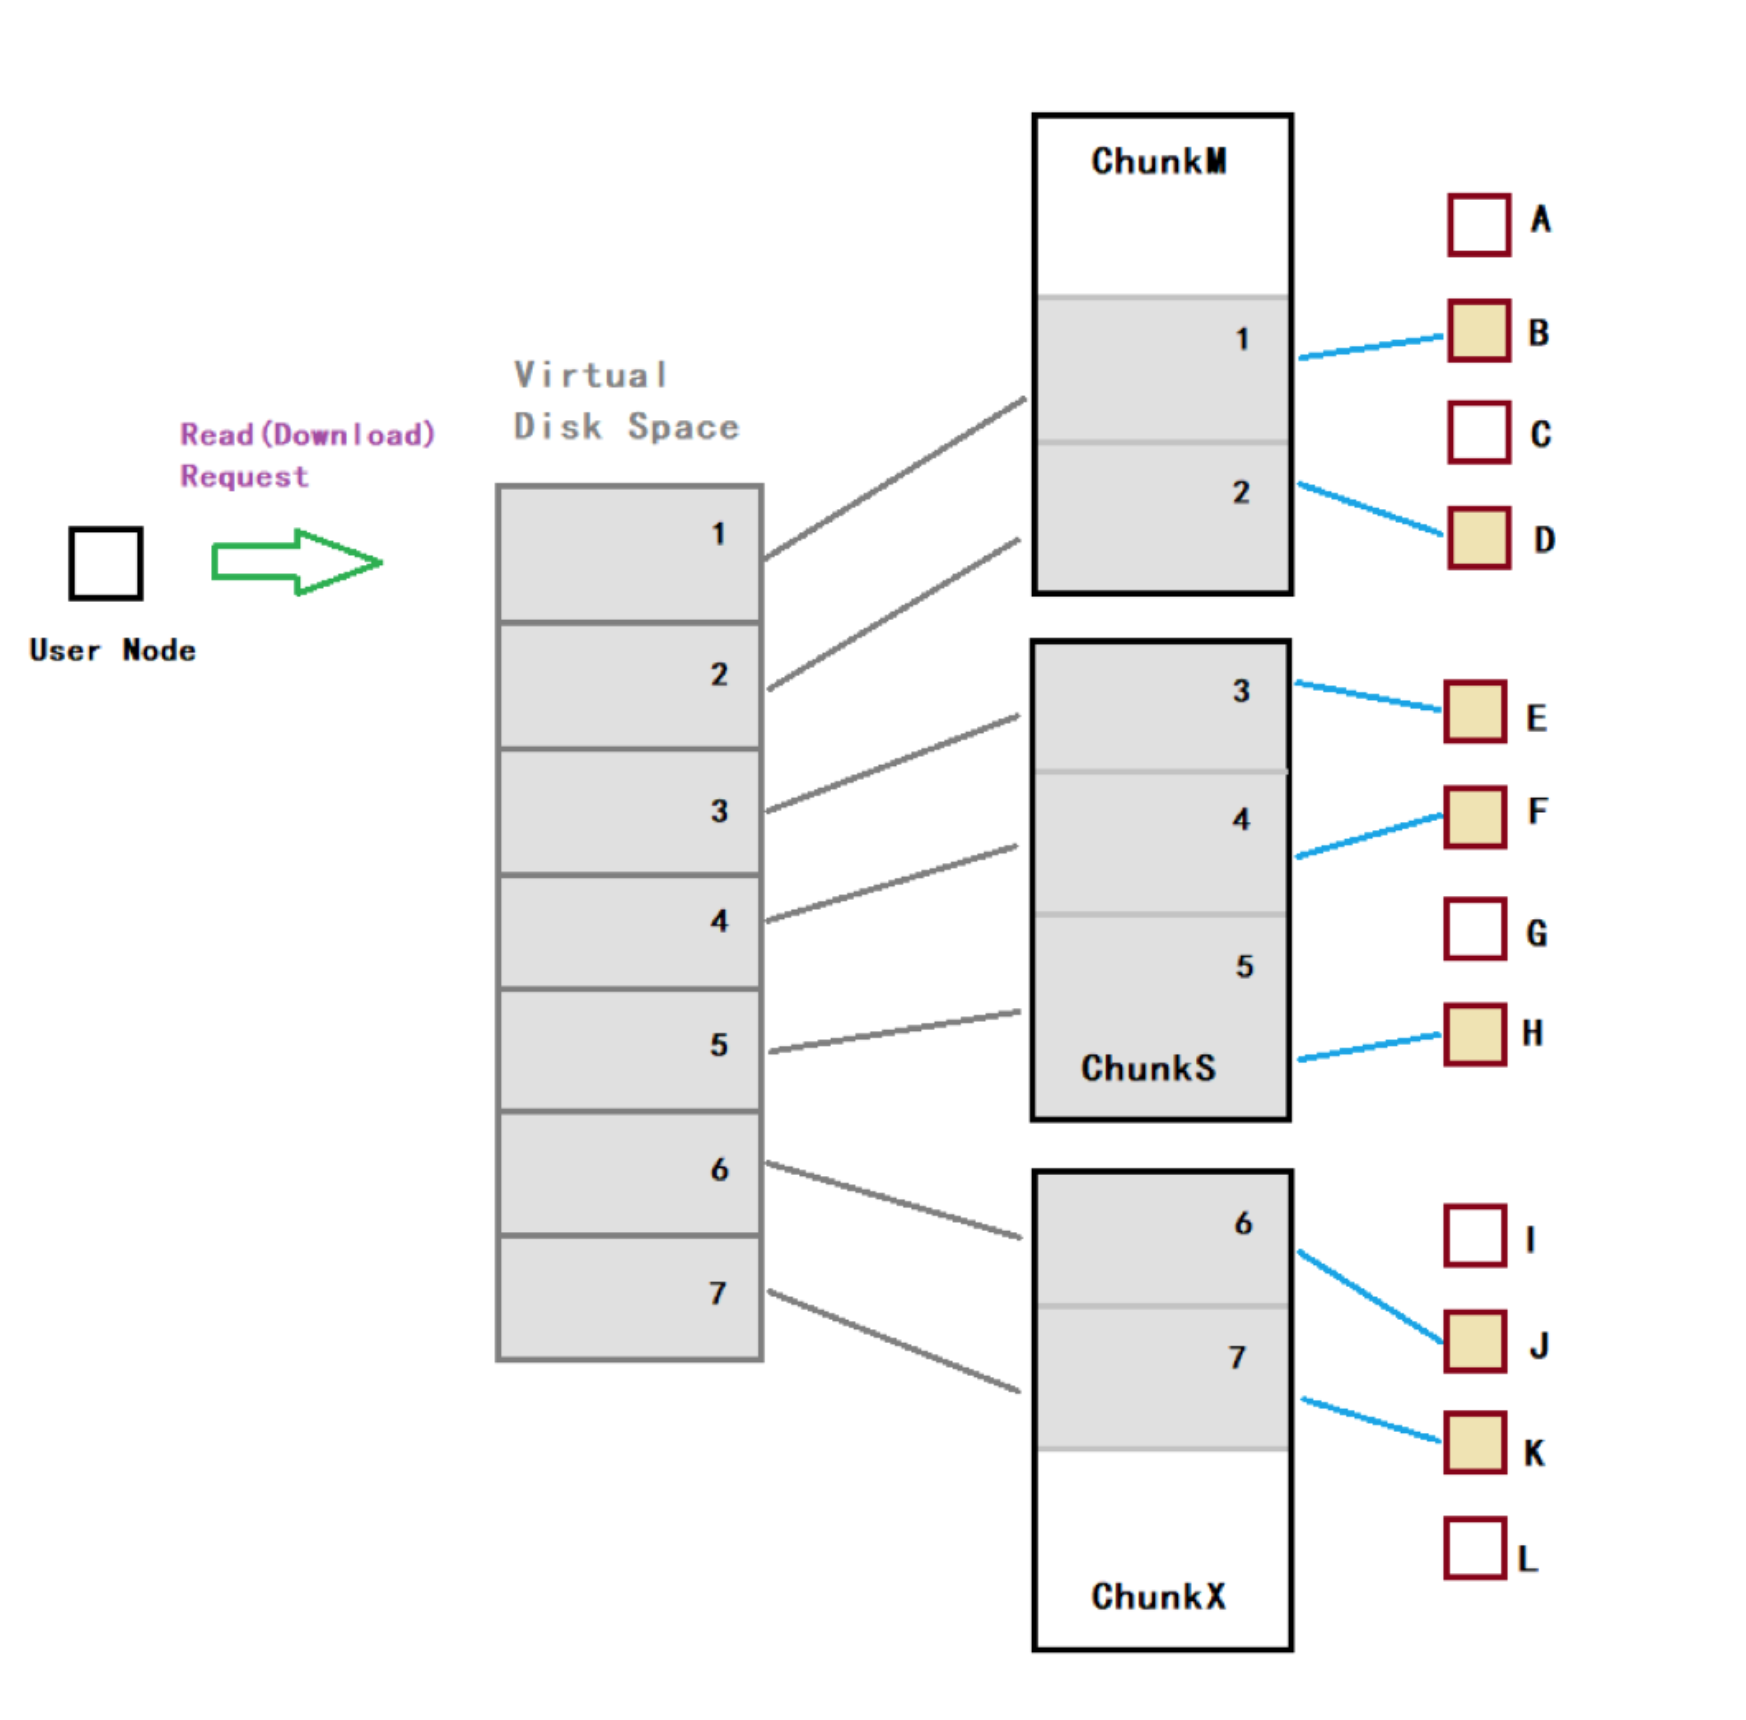
\includegraphics [width = 5in] {pic_cn/data_download.png}
\caption {数据下载} \label {fig: d6}
\end {figure}


\subsubsection{数据上载}

如上图所示,16PB虚拟空间中包含有很多Chunk, 每个Chunk是一个固定容量(比如1MB大小),对于存储矿工节点而言,它们贡献空间的方式就是贡献块副本,图中每个Chunk都由多个矿工贡献的块副本构成,所以Chunk是一个逻辑概念,它代表的是虚拟空间中的一段,比如Chunk1 表示虚拟空间中的0-1MB这段空间,而Chunk2则表示虚拟空间中的1MB-2MB的空间…;每个Chunk都可以由多个矿工提供的1MB块来构造,副本数量可伸缩,根据不同阈值来做不同的认领策略。


\begin {figure} [htbp]
\centering 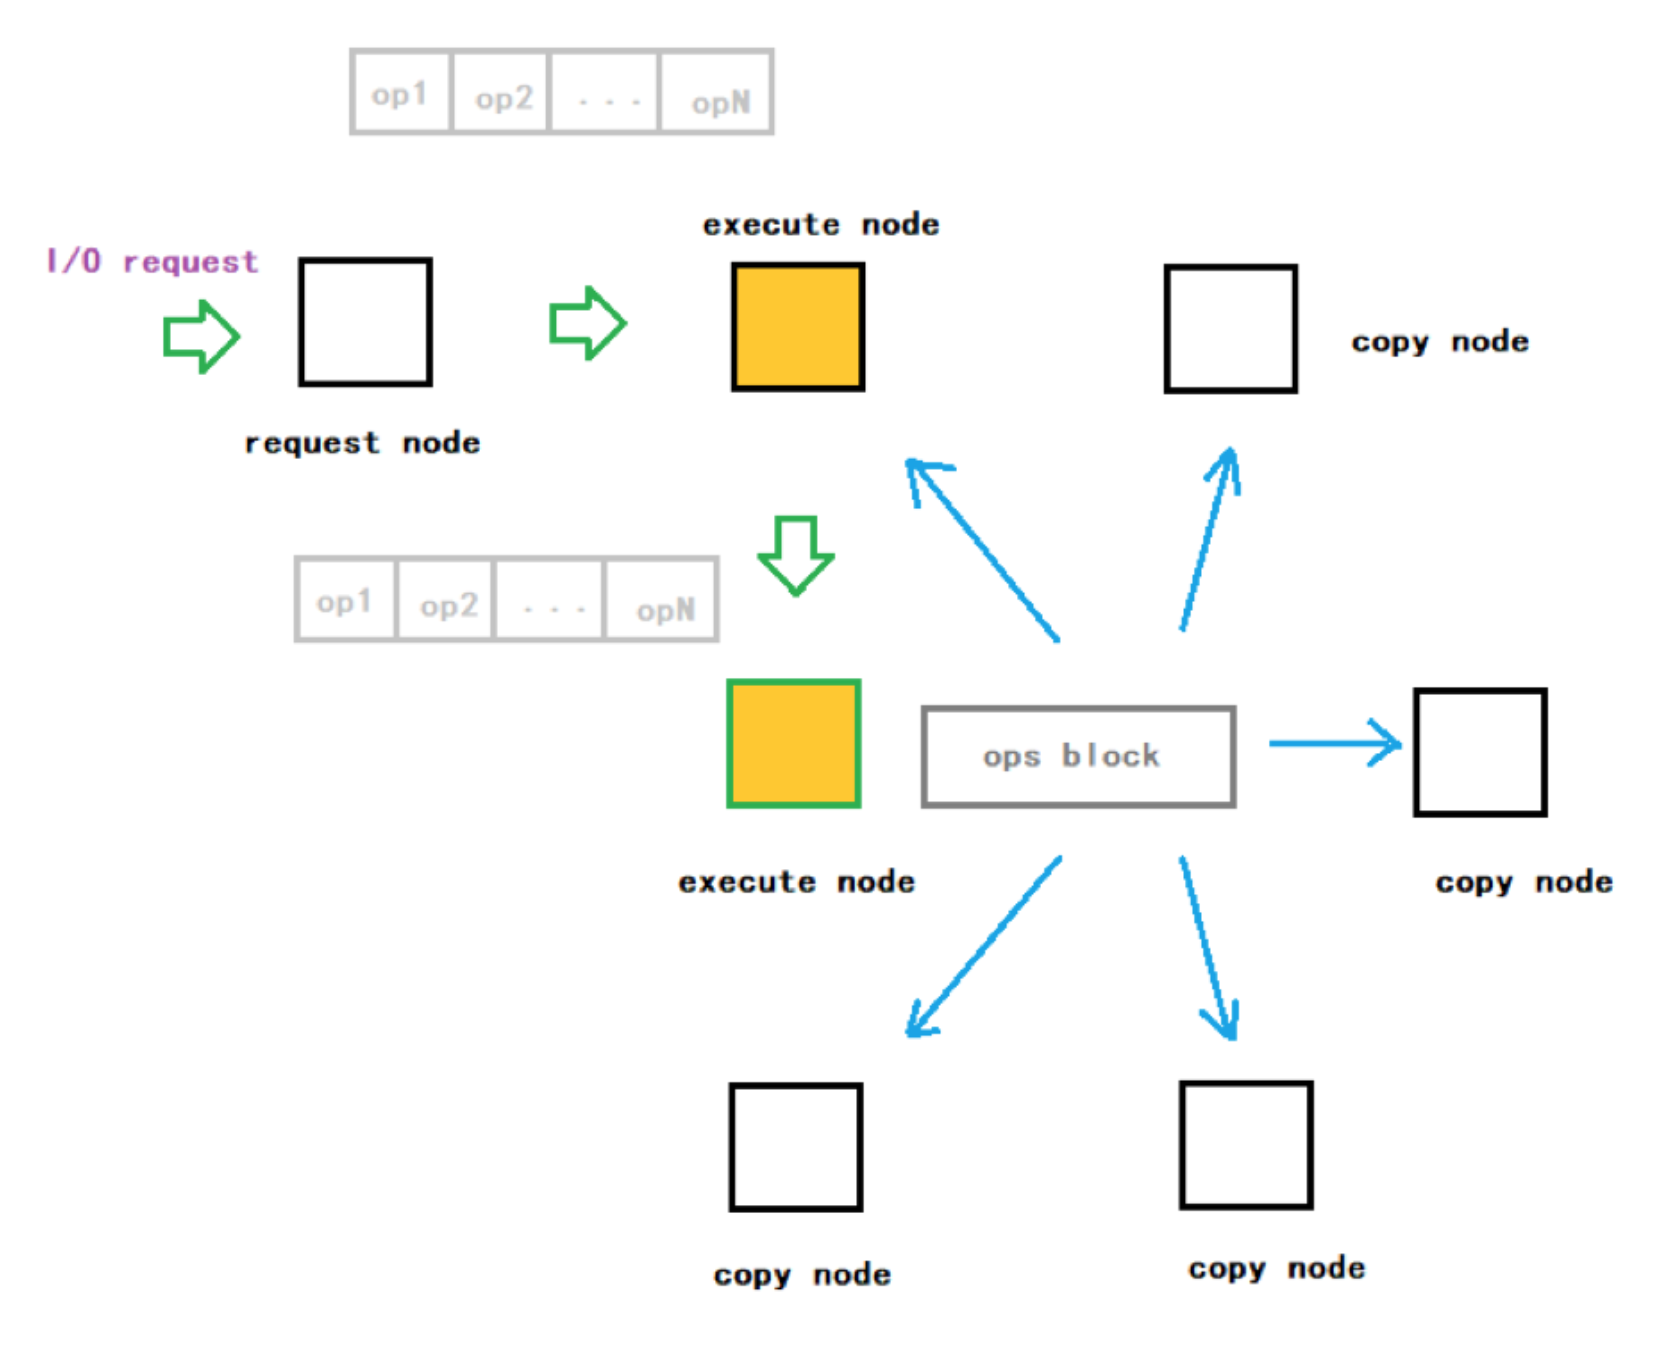
\includegraphics [width = 5in] {pic_cn/data_upload1.png}
\caption {数据上载} \label {fig: d7}
\end {figure}


\begin {figure} [htbp]
\centering 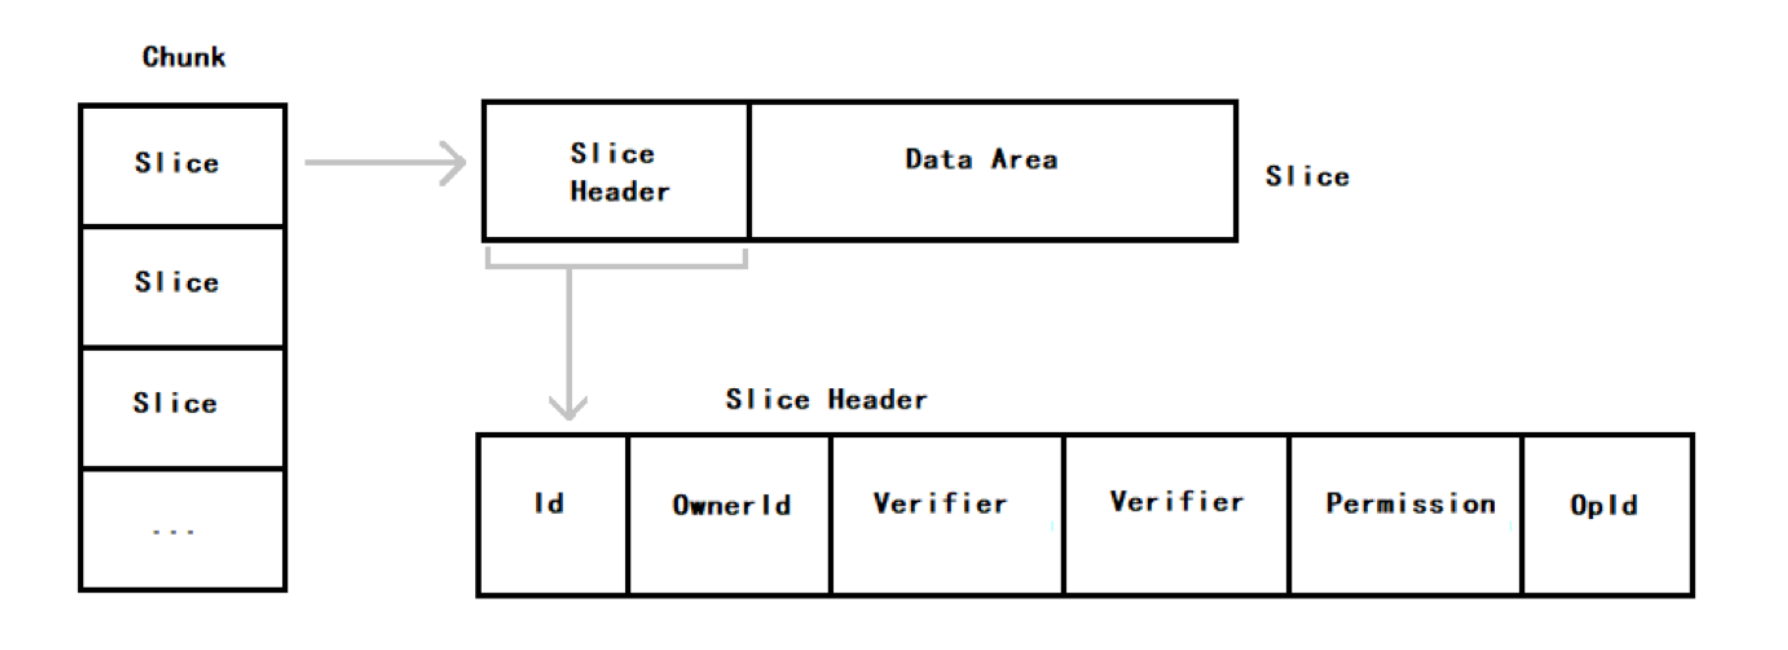
\includegraphics [width = 5in] {pic_cn/data_upload2.png}
\caption {数据上载(继)} \label {fig: d8}
\end {figure}

数据写入流程描述:

我们将 Chunk 划分成若干个Slice, 而Slice是用户端操作的基本单位,Slice的OwnerId就是这个Slice的租户和使用者,只有他有权限来更新和写入这个Slice,服务模型这样的:


\begin {figure} [htbp]
\centering 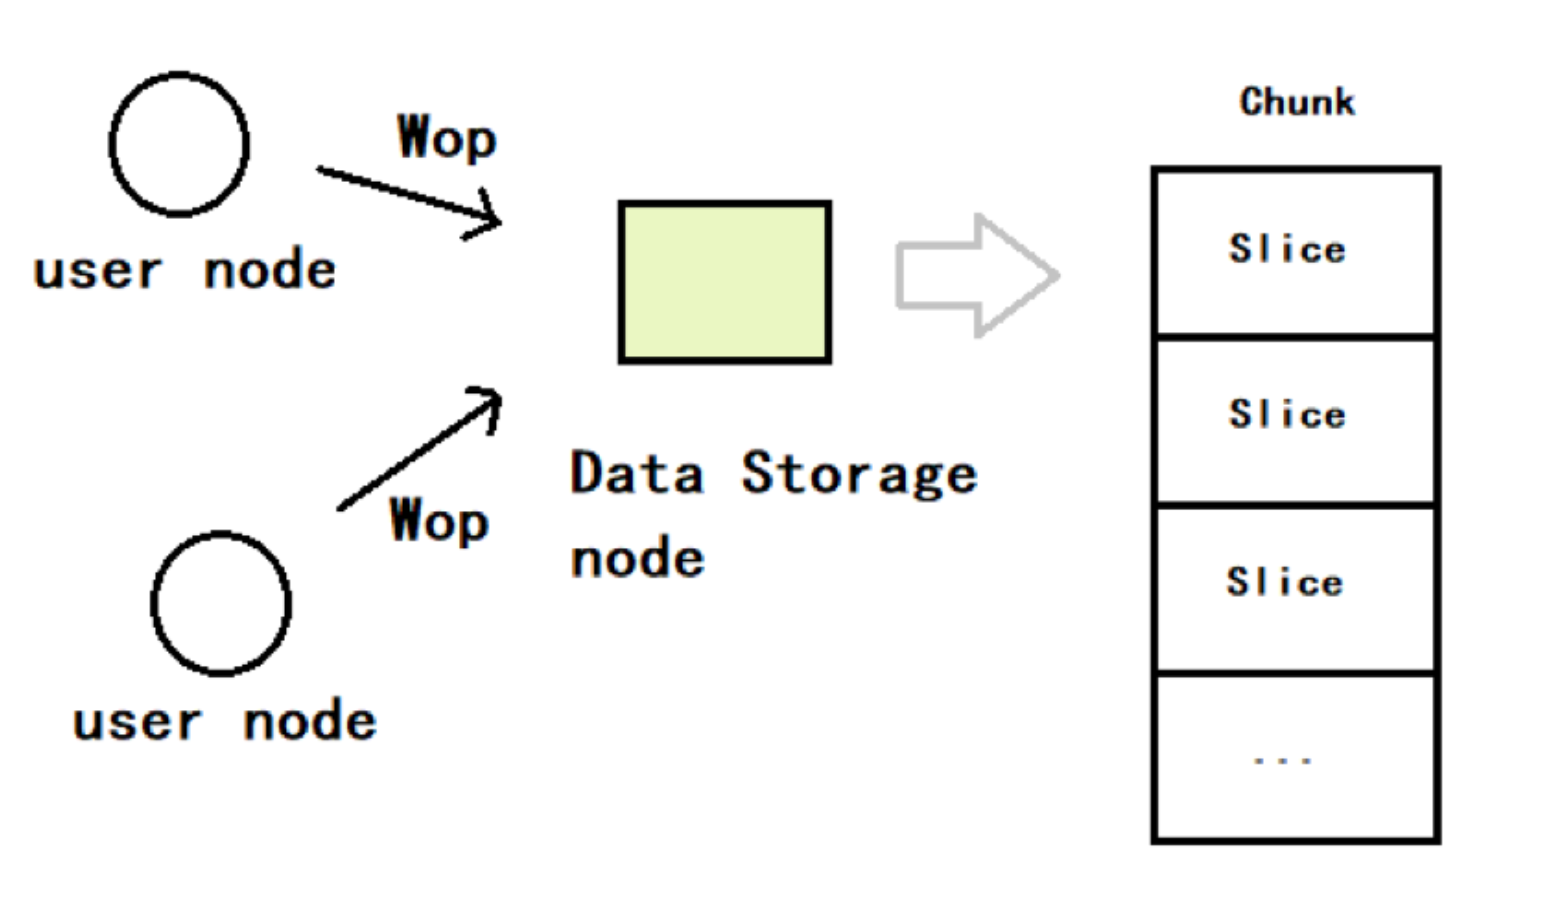
\includegraphics [width = 5in] {pic_cn/data_write.png}
\caption {数据写入} \label {fig: d9}
\end {figure}


对于Chunk而言,用户直接访问存储节点上的Slice,这样就不存在任何障碍和欺骗。
而对于会话服务来说,服务模型变成如下:

\begin {figure} [htbp]
\centering 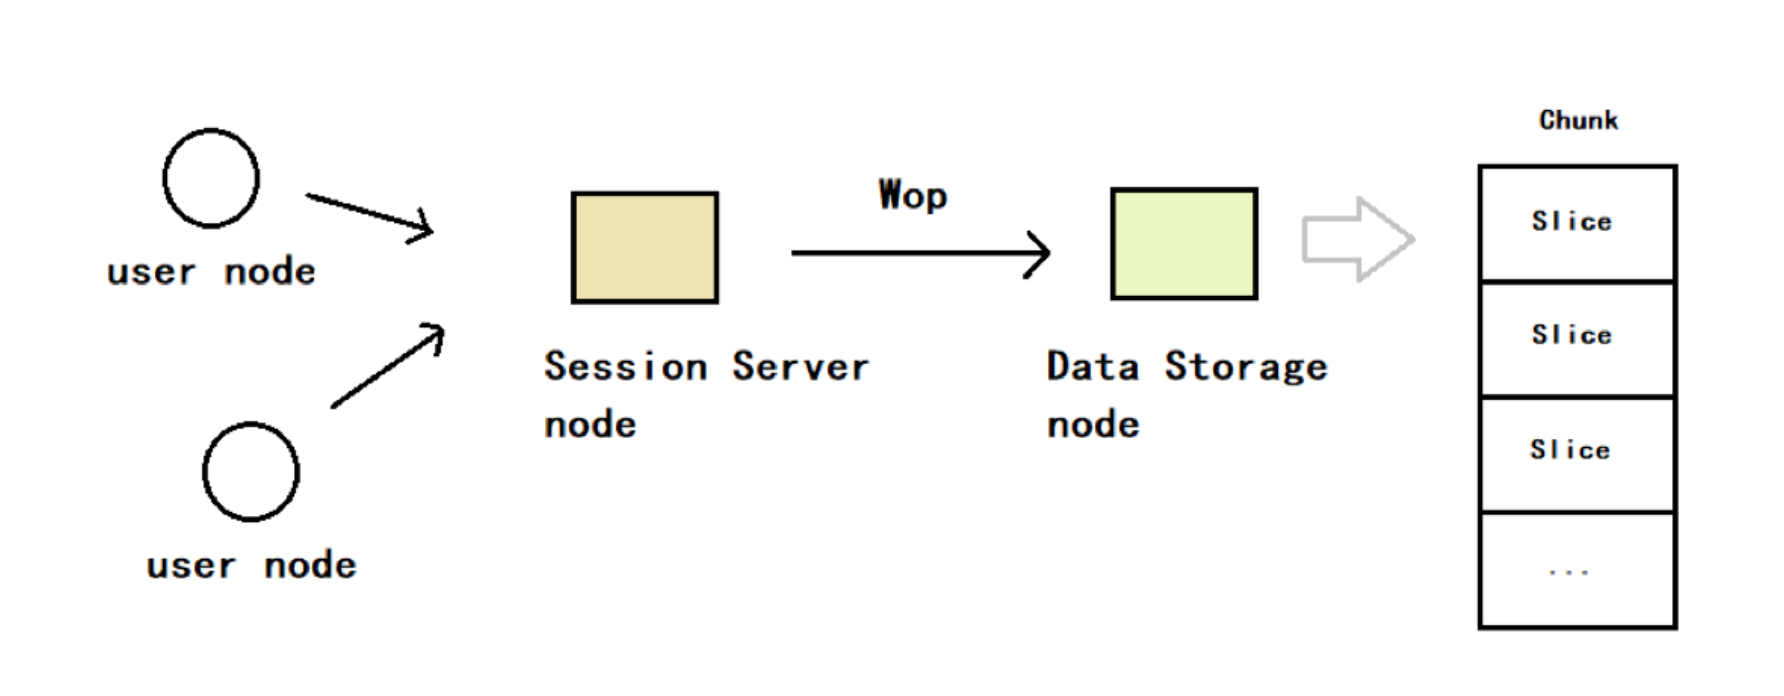
\includegraphics [width = 5in] {pic_cn/node_visit.png}
\caption {数据节点访问} \label {fig: d10}
\end {figure}

如图所示,所有的用户都要在会话服务节点通道服务器上进行交流和通讯,而会话文件数据则需要依靠会话服务节点来提交给存储节点。

会话服务节点是从通道区块链中根据动态路由随机挑选出来的节点,它的行为不可预测,所以我们并不能充分信任它不会作恶。虽然会话内容都是加密传递的,它虽然无法窥探会话内容,但它可以在写入时恶意破坏存储节点上的会话数据。

请求端通过构造一个发起问询指令广播发送给同一个块复制组的成员节点,通知它们操作者Id。各节点接收到指令,如果当前没有人使用或者最近操作距离当前时间已经超时,则签名给予接受。并将签名的回应消息通过主动寻路传递给请求端或者按广播路径原路返回请求端,请求端接收足够数量的签名后,将所有签名打包,形成一个Open指令再次广播,各节点检查验证签名并确认数量,符合2/3同意则设定操作者Id到内存。

块副本同步的设计:将同一个块数据组的所有参与节点看作针对这个数据块的一个微型区块链,该区块链采用半缓存式的同步策略,每个组节点都可以收集来自各个请求端的Wop请求,收集后开始广播这些Wop到当前区块的执行节点;执行节点收集到请求后,将它们按照接收顺序打包成操作区块(利用排序消除多节点可能对同一虚拟写入产生的冲突),打包同时过滤掉不符合分片权限设定的操作

每个组节点 都可以称为一个副本矿工,它收集来自其他各个组节点的Wop请求,当Wop数量满足一定要求(N>0)并且收集时间满足一定要求的情况下,并将自己原发的或者接收到其他节点的Wop的Id打包成区块广播给其它节点,同时按照区块中Wop的排列顺序执行各个Wop到本地。


\begin {figure} [htbp]
\centering 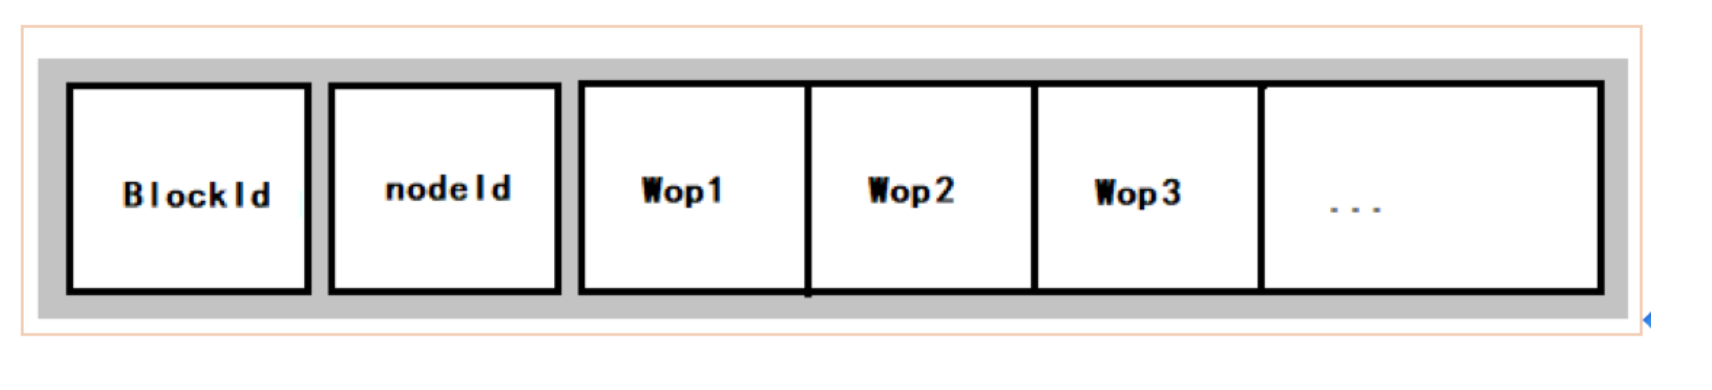
\includegraphics [width = 5in] {pic_cn/execution_sequence.png}
\caption {顺序执行} \label {fig: d11}
\end {figure}


如果组节点在创建并执行了自己生成的Block后,又收到了来自其组节点的广播区块时需要首先判断自己的优先级。如果有节点发生了宕机,那么在它作为执行节点的时间窗口内无法产生区块,则所有操作都会产生一定延迟。针对这种延迟较高的特性,上层应用在加载数据前应该首先做好缓冲,尽量将加载次数减少,将大部分操作合并起来一起提交为宜。

而对于新加入的组节点,则需要有一个数据下载的过程,它从组节点中选择一个能够顺畅通讯的当作数据服务节点,开始从头下载该Chunk的完整数据;于此同时它也需要同时加入到这个集群,成为一个准集群成员节点(semi 组节点)。它需要在下载数据的同时,将下载过程中的所有区块都保存起来,下载数据完毕,再将所有区块都在本地执行一遍,这样就能够完成整体同步,并跟上其他副本节点的节奏。

执行节点 的选举规则比较讲究,所有的组节点可能数量较大,比如32个。如果采用简单的轮选策略,大多数情况下,接到IO操作请求的node就是少数一些跟app node绑定的节点(一个Chunk可能同时被多个租户使用,操作者并不唯一);所以我们需要选举一个leader当作本副本同步群的执行节点。选举过程:租户向虚拟磁盘写入数据的时候,会首先调用一个Open方法,Open方法会查询所有参与的Chunk信息所在的所有副本节点nodeId,并向这些存储节点发送Open消息(带上chunk, slice),存储节点收到后根据消息中携带的(Chunk, slice)信息从本地磁盘中找到相应本地存储记录并进行属主和属性(读写权限属性等)比对,根据比对结果做不同的动作;如果验证合格,就将这个节点加入到该(Chunk-Slice)的执行节点 组中,并将该消息周知所有的节点,一个Slice分片中的执行节点组中的成员轮流出块,出块成功即分工广播:广播机制可以设置为询问传递模式,因为涉及到带宽和流量,所以传递前先沟通询问,而不要直接扔数据,对于组节点来说尽量只挑选1-2个下级节点进行数据传递,然后由下级节点再做进一步传递。

从上面的描述来看,写入操作流程比较复杂,如果应用层采用同步等待,会让效率比较低,应用层应该采用缓存操作的方式,一次性提交所有缓存操作后,一方面继续等待并加入新操作指令进入缓存区,一方面等待区块下发确认之前提交的操作得到执行并从缓存区清除。

\subsection{时空证明、存在性证明及可获取证明}
\subsubsection{时空证明和存在性证明}

空间同步分为三种类型的同步
1.	没有被使用的时空证明
这种情况下,空间只是作为资源存在,还没有用户租用或者租用了还没有写入数据,所以不能由一套确定的数据来验证它,需要提供一种副本之间的自验证机制。
2.	已经在使用的时空证明
已经在使用的空间,表示该Chunk已经被用户租用,并且已经往空间提交了(文件)数据,所以同步和验证都是基于这些数据来进行。
3.	正在读写的空间证明
正在读写的组节点,只有占多数的节点更新后才被认可。

任何空间提供者提供的空间都被数据填满,这些数据可能是用户数据,也可能是自动生成的填充数据。区块链将定期发起(例如每20个块)一次随机抽查,让一个数据组内相互验证,占多数者被认为是可信节点,可以获得空间奖励。

\subsubsection{可获取性证明}

数据空间的使用者在每次结束数据代理的雇佣后者会提交一个使用期间的服务数据,并写入世界状态,主网将自动将服务体验不好的空间挖矿者打入黑名单。服务质量越不好,服务质量的提交速度越快,能够越快找出害群之马,随着时间的推移,不可信的空间挖矿者将难以对系统造成伤害。

\subsection{激励机制及付费机制}
\subsubsection{空间使用机制}

空间的使用机制如下:

\begin{enumerate}
\item 首次空间使用:用户用CNT按内置的价格公式支付对自己的存储对象按时间长短和空间大小进行付费,付费存入资金池,区块打包时确认存储对象到期时间戳。
\item 空间调整:当对象扩大或缩小时,根据对象变化、追加的CNT,根据计价公式改变时间戳。
\item 空间锁死:时间戳到期后空间访问权自动锁死,空间将作为可申请空间标记。
\item 空间回收:新的空间认领时会先使用空闲空间,然后使用到期比较早的空间。
\item 空间解锁:当用户申请续费时,原有的空间如果没有被回收,可以再次被找回来,但需要补缴从过期到当前时间的空间费用。
\item 地主奖励:按已经购买使用权每个区块时间注销的数额乘上价格得出奖励总额,通过随机验证机制确认给通过验证的地主。
\end{enumerate}


\subsubsection{相关变量约定}

所有空间购买的付费交易将由专门的算法完成并记录在主链上。付费将进入专门的称为“资金池”的帐户。该资金池记录空间购买行为。以下使用兆天(MD)作为空间使用权的计量单位,兆天表示一个兆空间一天的使用权。

变量假设如下:

\begin{enumerate}
\item W:假设用户可使用的世界硬盘的总空间为WD,单位MB字节,该数据每个区块修正一次,由区块头记录。Worlddisk首字母。
\item $t$及$T_{-1}$:分别表示本区块时间戳和上一区块时间戳。 
\item T:为当前区块一年总兆天数。这里规定一个空间对象最多能申请的保存周期为交易时算起的365天以内,所以每个区块周期所能提供的兆天最多为365W,我们用T表示这个空间使用权,该数据每个区块修正一次。$T = T_{-1}+(W-W_{-1})*(t-t_{-1})/(24*60*60)$。$T_{-1}$为上一区块的兆天总数,$W_{-1}$为上一区块的世界硬盘的总空间。$(W_0-W_{-1})*(t-t_{-1})/(24*60*60)$为当前区块新增减的兆天。T为Total首字母。
\item B:为当前区块已经购买且尚可使用的兆天数,该数据每个区块修正一次,由区块头记录。$B = B_{-1}-B_{-1}*(t-t_{-1})/(24*60*60)+\Delta B$。其中$B_0$为当前区块的已经购买尚可使用的兆天数,$B_{-1}$为上一区块的已经购买尚可使用的兆天数,$B_{-1}*(t-t_{-1})/(24*60*60)$表示当前区块需要注销的已经使用的兆天。$\Delta B$为当前区块新购买兆天数。B为Bought首字母。
\item R:表示当前区块剩余未够买兆天,包括空闲空间和已经到期的空间。Residual首字母。R = T - B
\item M:表示当前区块资金池中的CNT代币数。
\item p:表示当前区块存储单价,每兆天的使用价格,单位为CNT,这里表示硬盘使用者,即“市民”每兆天的“租金”费用。
\item r:表示当前区块单位租金,每兆天的出租收入,单位为CNT,这里表示硬盘提供者,即“地主”每兆天的“出租”收入。
\end{enumerate}

\subsubsection{对空间使用权价格函数的要求}

兆天价格是调节存储空间使用的关键,价格的调整要满意以下几个条件:

\begin{enumerate}
\item 随着使用需求的提高,价格以非线性方式不断提高,以使空间永远处于富余状态。
\item 随着使用需求的提高,时空验证的奖励提高,以促使更多地主入住。
\item 空间租用价格处于合理区间。
\item 空间租用价格处于较为稳定的状态。
\end{enumerate}

\subsubsection{Bancor付费机制}

如果每个存储对象所能存储的时间是没有限制的,那么很难对流入量进行管理。如果规定每个对象所有存储的时间最多为365天,超过的需要续费,所有能购买的兆天共为T=365W。由于在每个出块周期都有固定的兆天总数,就可以在每个出块周期采用类似Bancor的机制来对兆天进行定价。

Bancor是以太坊的一个项目,是一个货币系统,通过智能合约为数字货币提供持续流动性。Bancor解决了交易量小的数字货币的流动性。它不需要第三方的机构,也不需要第二方,通过智能合约就能买卖Token。但同时,Bancor的自动调节机制使的自动价格发现和自主流动机制成为可能,也使其永远不会售罄。

以下利用Bancor机制在某个出块周期对兆天进行定价。% 参考:https://www.jianshu.com/p/7a535407d732

Bancor需要一个常数项:$c=M/(p*T)$

通过上面两个公式就可以推算出价格公式:$p=M/cR$

当参数c值不同时,价格曲线变化如下:

\begin{figure} [htbp]
\centering 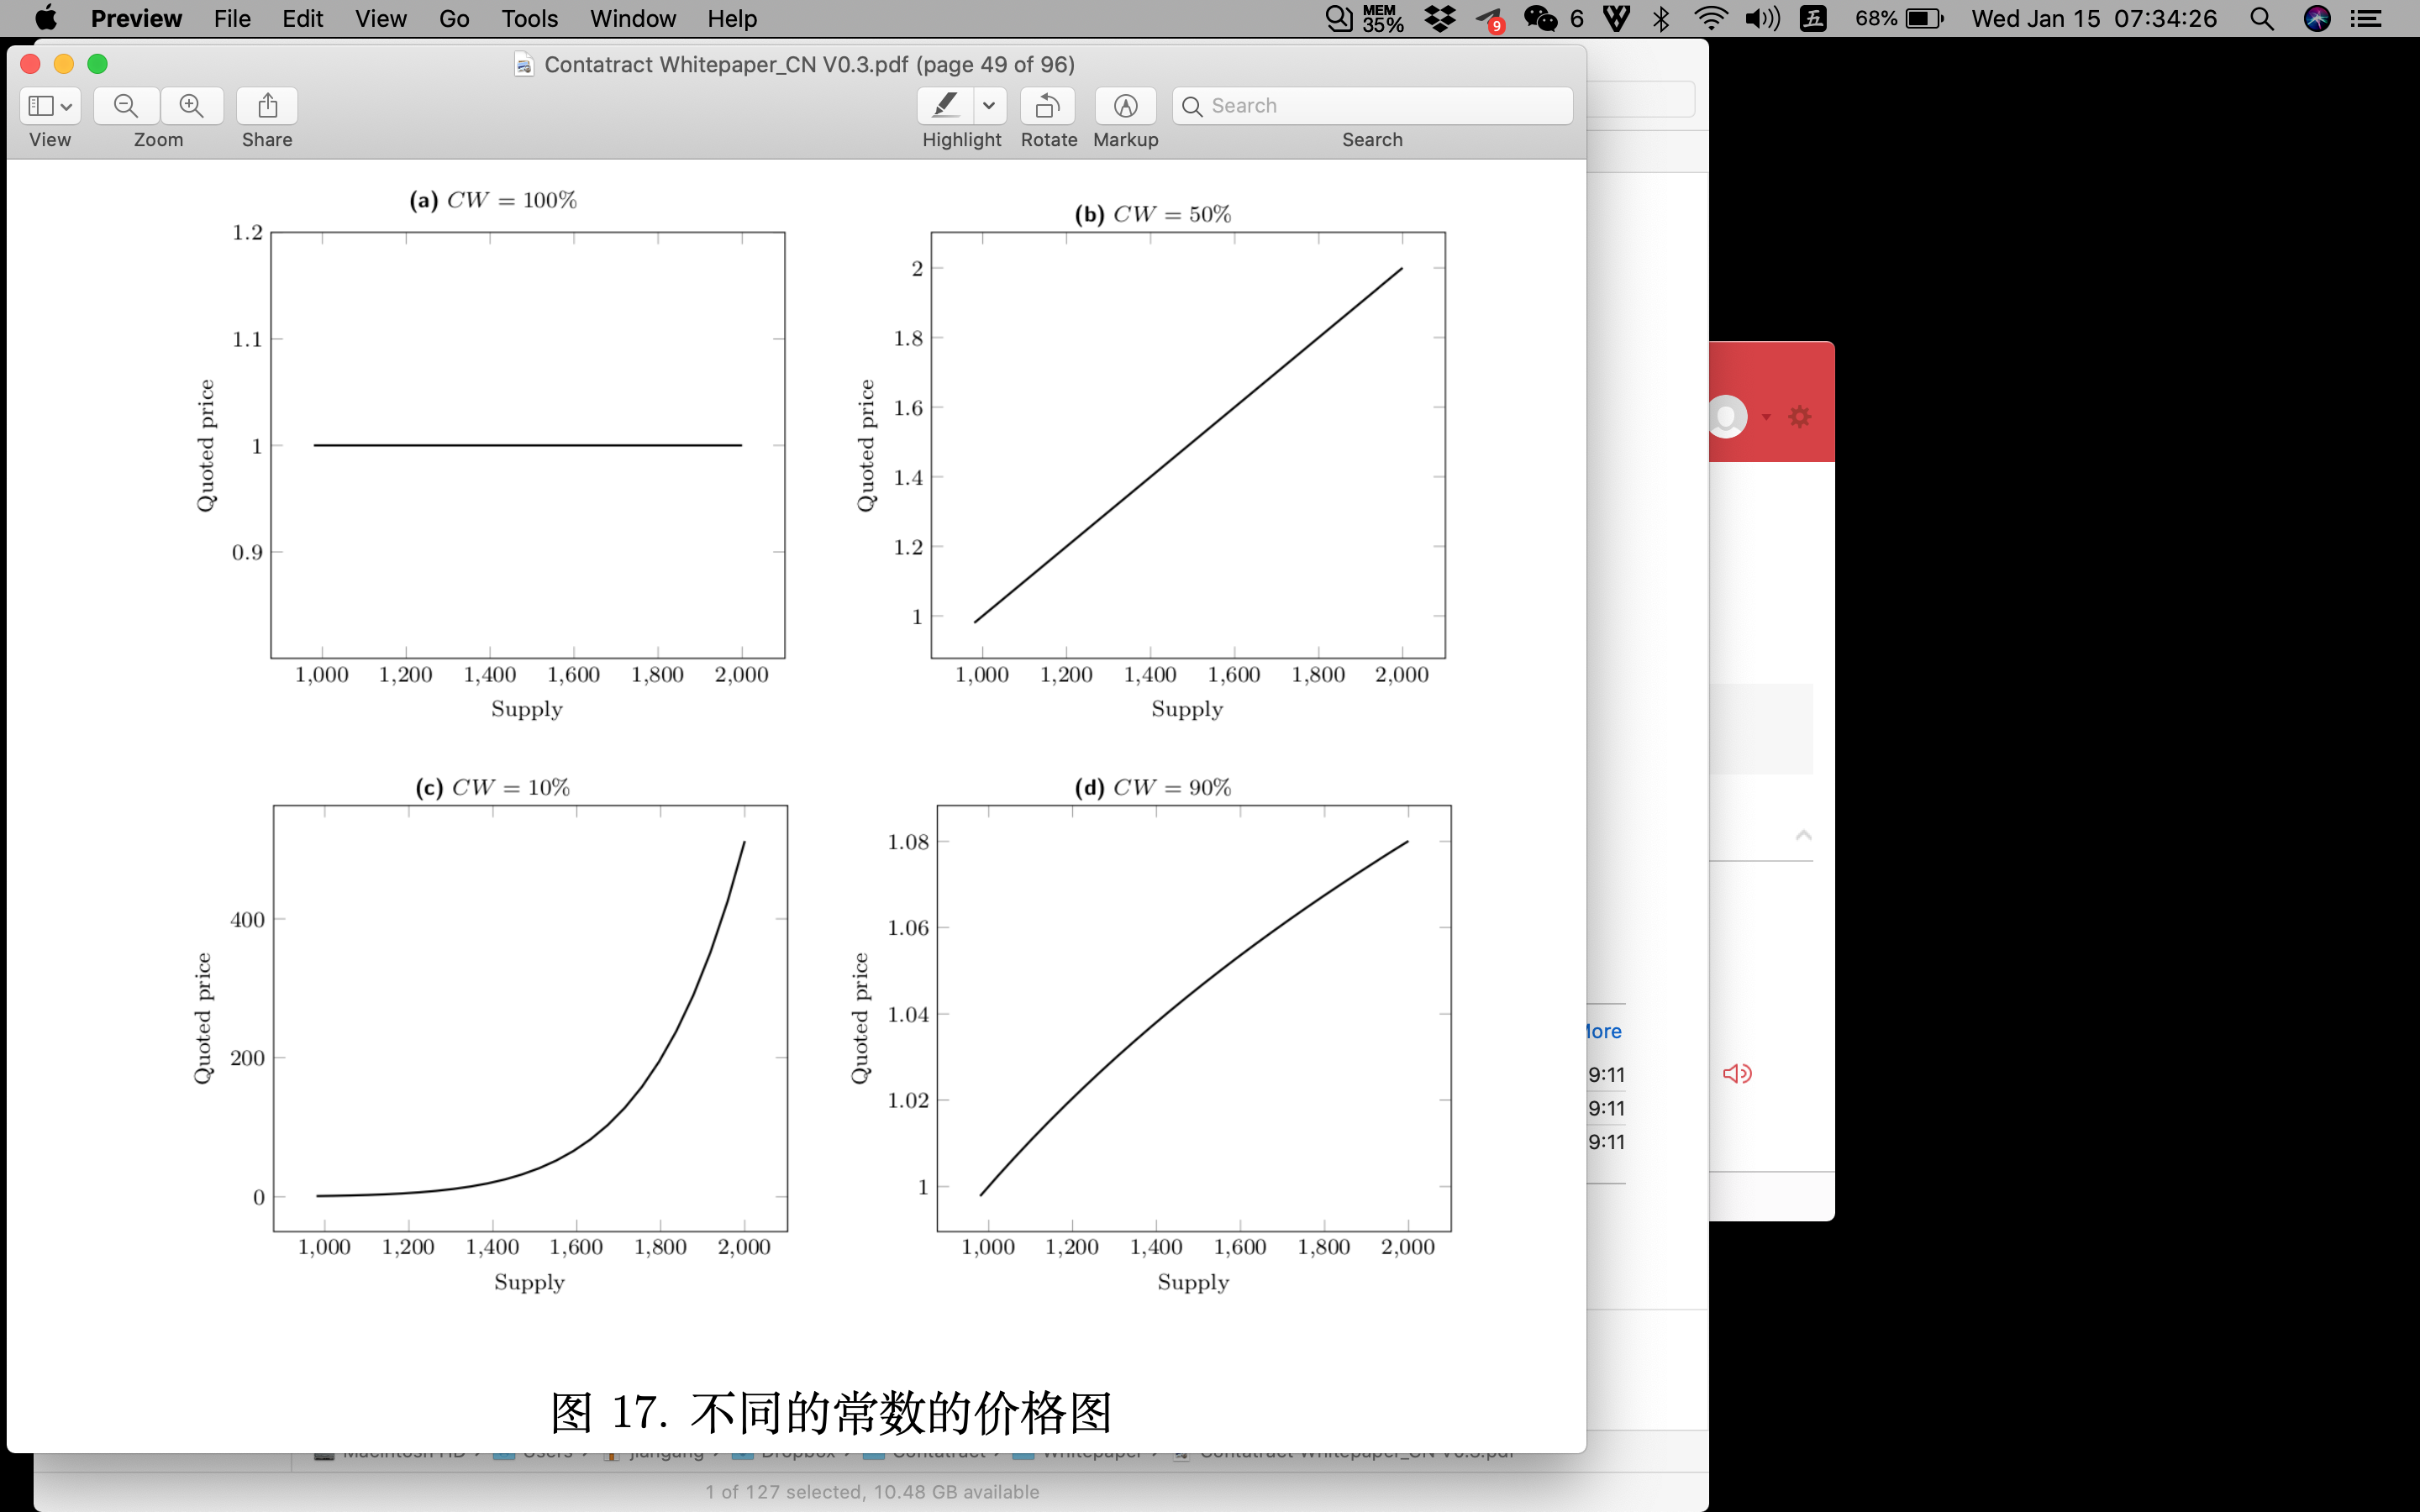
\includegraphics [width = 5in]{pic_cn/different_CW.png}
\caption{不同的常数的价格图} \label{fig:different_CW}
\end{figure}

其中CW表示常数:

\begin{itemize}
\item 当 CW = 100\%,可以认为发行代币是连接器代币的别名,不管需求如何变化,所发行代币的价格总是等于连接器代币的价格。
\item 当 CW = 50\%:所发行代币和其供应量呈线性关系。
\item 当 CW < 50\%,图中 CW = 10\%,随着供给的增加,价格增长迅猛。
\item 当 CW > 50\%,图中 CW = 90\%,随供给的增加,价格变化小。
\end{itemize}

我们可以把参考Bancor中常数,包c设为20\%左右,以使当使用存储的人很少时,存储很便宜,但使用人越多越贵,而且是非线性增加的。

由于Bancor协议中每买入一个数量兆天都会引起价格变化,我们采用简化的算法,即每个出块时间里的价格都相同。

\subsubsection{地主租金、地主补贴、捐赠通道}

\textbf{地主租金}

由于世界硬盘使用率为B/T,但整个硬盘的费用需要由真正使用者负担,所以应该由资金池支付。

由于每个区块按时间戳已经自由销毁已经过期的使用权,这些销毁的部分应该支付给硬盘提供者。其需要支付的兆天数量为:

$$r=(t-t_{-1})/(24*60*60)$$

针对上一区块进行清算,上一区块已经卖出的兆天为$B_{-1}$,已经收入的代币为$M_{-1}$,所以这部分兆天应该从资产池里按比例支付,即应该产生的租金费用为:

$$r=M_{-1}*((t-t_{-1})/(24*60*60))/B_{-1}$$

这些费用将在每个出块时间分散奖励通过验证的地主钱包。

\textbf{地主补贴}

为了让空间始终有一定富余,也使项目前期存储空间比较便宜,在一定期间内,向资金池定期增记一定数量的资金,以使整个生态可以补贴地主。

\textbf{捐赠通道}

分布式存储是项目的基础,也是很多人的梦想,我们可以增加一个捐赠通道,以使持币者可以将资金捐赠到资金池。

\section{基于分布式存储的分布式通讯}


\subsection{异步通信:Email}

分布式Email主要通过做交易将短信息(目前定义为小于1k)上传到世界状态,大的信息作为附件,由收件方到发邮方的个人云空间下载。下载分为免费和付费,数据通过收邮方的公钥加密保护。在付费的情况下,只有支付费用才能够拥有访问权。通过这种方式,可以实现数据的交易。

由于需要知道公钥,任何地址都可以申请附加的Email地址和Email别名,并将这个地址的公钥一同写入世界状态。

分布式Email的框架如下图所示:



\begin {figure} [htbp]
\centering 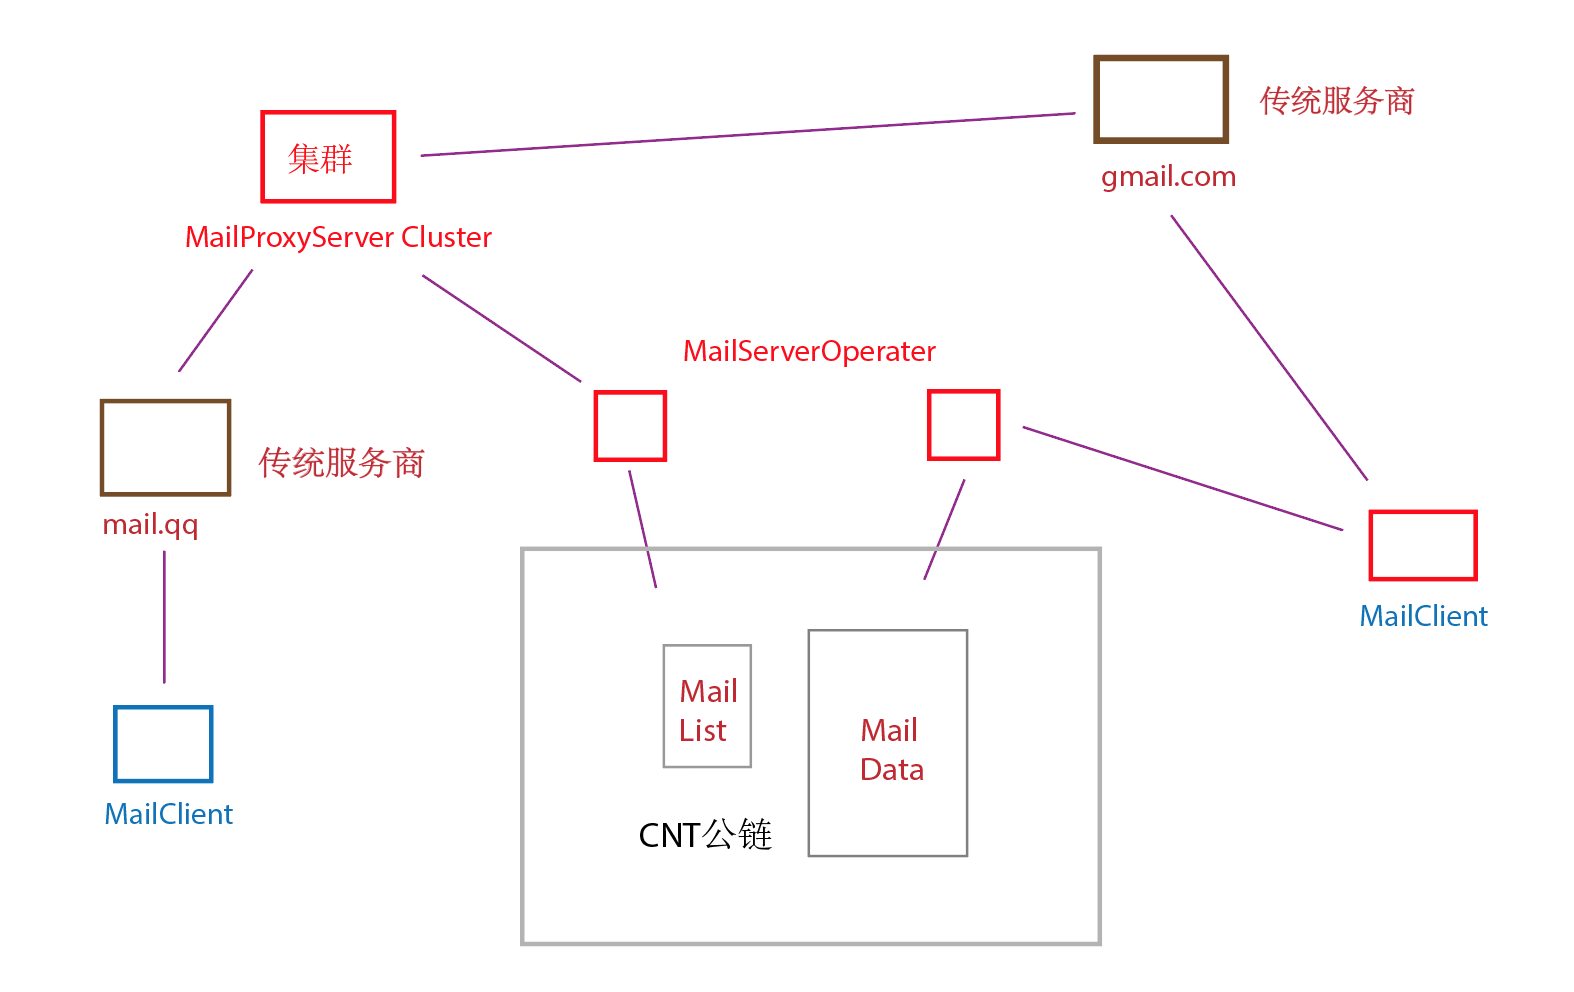
\includegraphics [width = 5in] {pic_cn/cnt_email.png}
\caption {CNT分布式数据路由框架} \label {fig: email}
\end {figure}
\subsection{数据路由的框架}

分布式社交,顾名思义,主要体现形式就是即时通讯,最古老的即时通讯出现在上个世纪90年代,用户之间建立的会话利用的对等网技术,中间不提供服务器转发,也就是我们经常提到的点对点技术。服务器只是起到一个用户电脑之间相互寻找和定位的桥梁的作用。虽然即时通信的大部分功能主要将由其上的DApp实现,但由于CNT因为拥有分布式存储的功能,具备了提供分布式通讯的能力。


\begin {figure} [htbp]
\centering 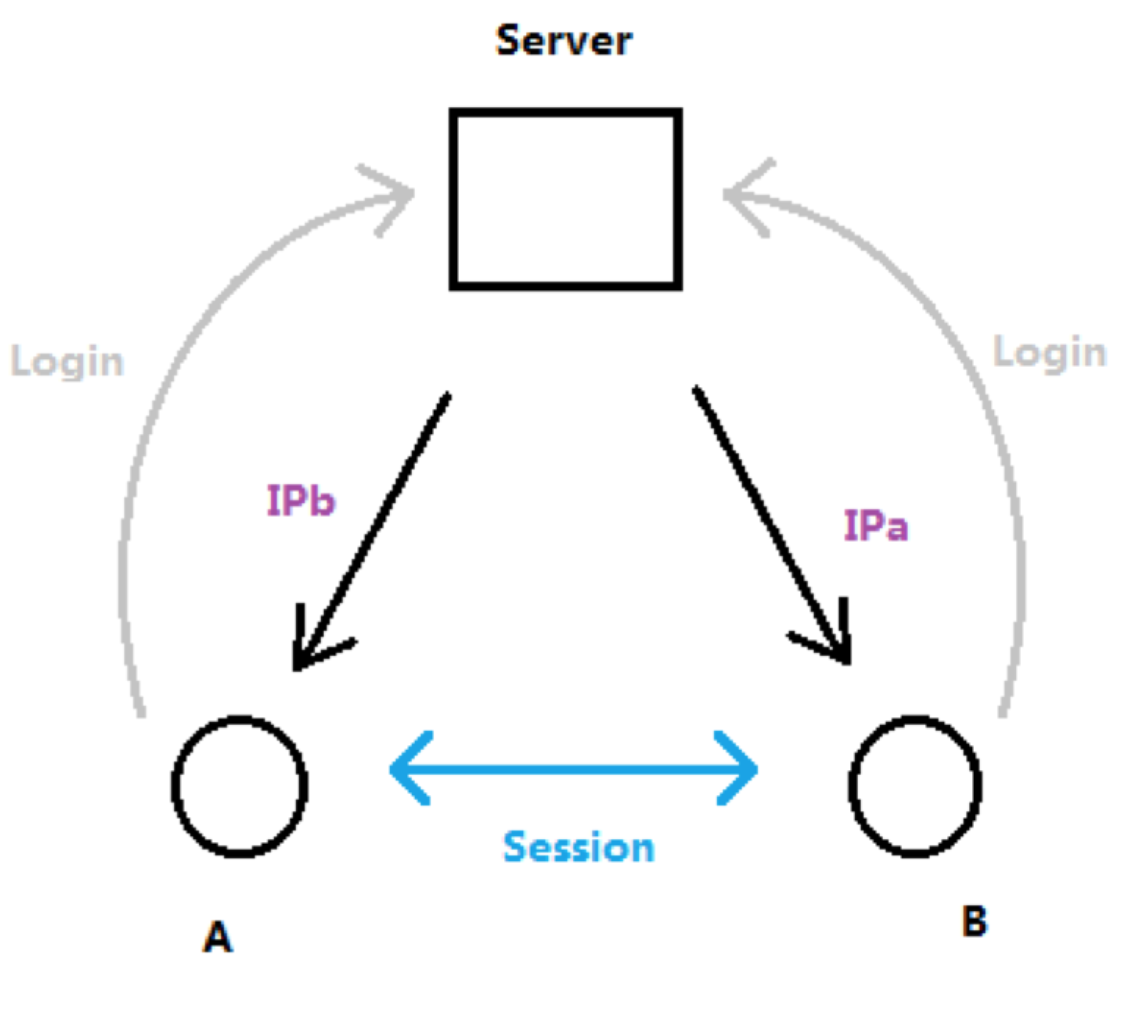
\includegraphics [width = 5in] {pic_cn/c1.png}
\caption {点对点对话} \label {fig: c1}
\end {figure}

如上图所示,AB节点仅仅是通过登录Server将自身的IP:Port传递给Server, 建立Session会话的时候从Server获取到对方的地址,它们建立直接通讯。这样做的好处在于,AB双方的通讯是独立于服务器的,没有任何的隐私泄露。

这种模式的缺点也很明显,那就是无法建立多人同时参与的会话,多人同时参与需要建立一个复杂的网状结构。如果采用以某个用户为核心的星型结构,那么当这个用户下线的时候,其他人的通讯连接又需要重新建立。而且这种纯粹依赖用户节点的模式还不利于实现会话参与人员列表的保存以及会话内容的保存。

所以最终即时通讯回到了中心化的聊天室模式。中心节点提供稳定的Online服务,提供会话内容的中转Relay, 保存Save, 管理Manager。这些强大的技术和体验优势是单纯的点对点所无法比拟的。


\begin {figure} [htbp]
\centering 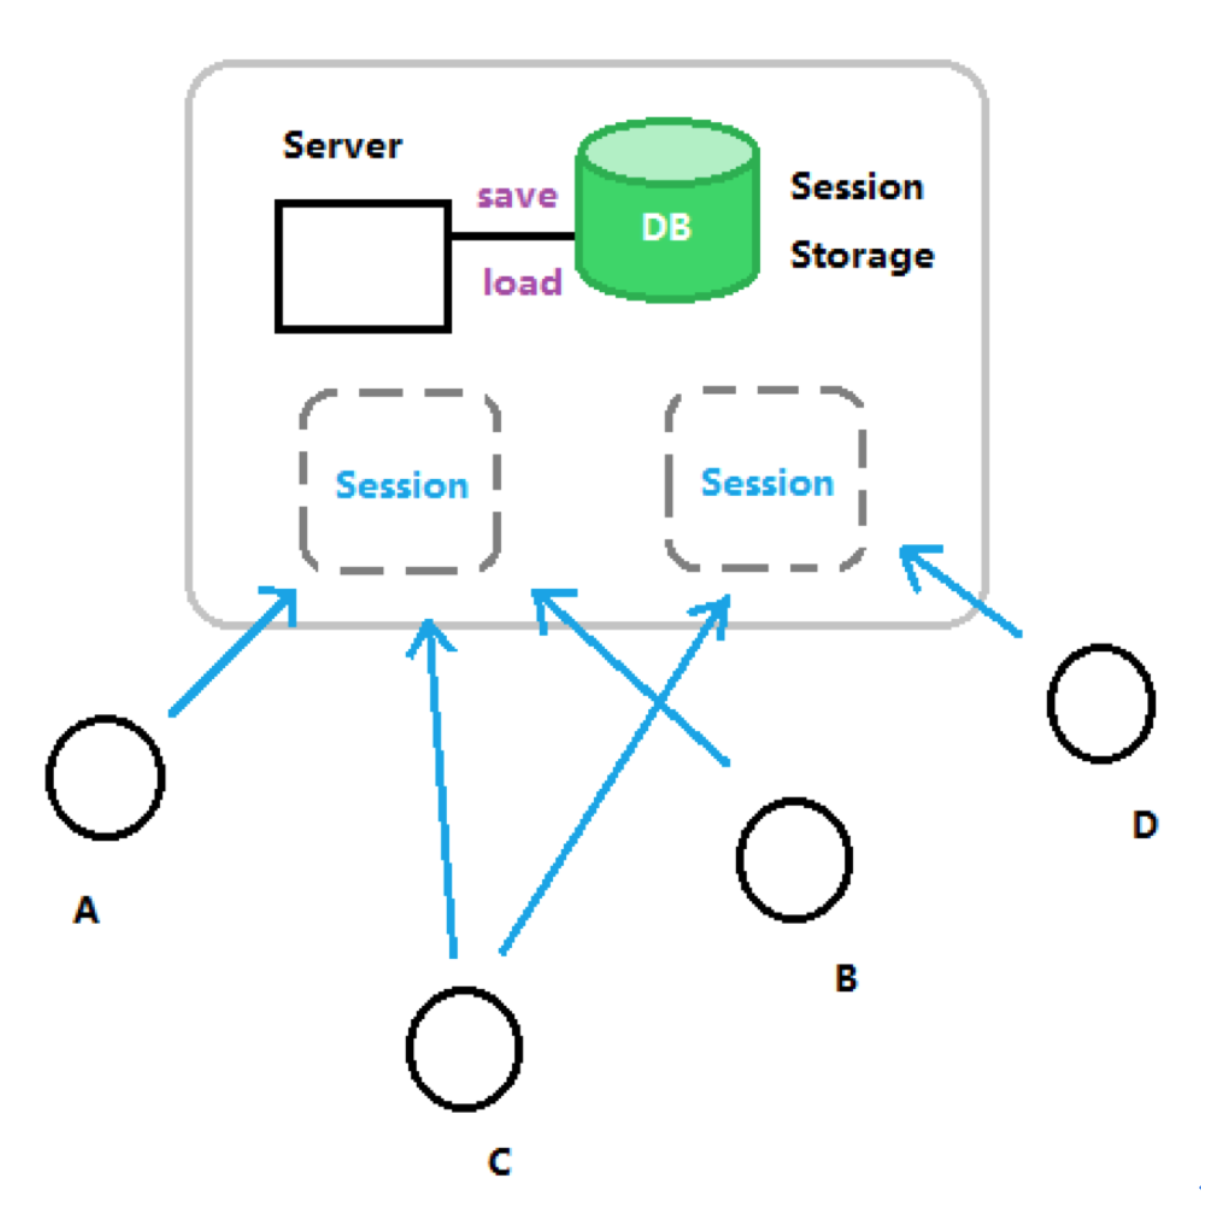
\includegraphics [width = 5in] {pic_cn/c2.png}
\caption {中心化会话服务} \label {fig: c2}
\end {figure}

中心化节点提供的会话内容存储服务和稳定的通道可用性使得用户会话功能变得非常可靠,而且功能强大。

对比一下上面两种模式,我们可以看出,对于用户节点而言,他们需要体验的正常会话服务,需要具备两个必要条件:1. 会话Session的保持;2.通讯通道服务的高可用;这两个条件上,纯粹的点对点难以满足,节点在线的不稳定造成拓扑结构的不稳定,保持Session的内容和配置对于普通用户节点就更加复杂(如果保存在它们自身,则面临复杂的同步问题)。而中心化服务这两者都能完美解决。所以传统的IM服务都是统一由中心服务器提供,中心服务器的优势在于逻辑处理协调一致,存储服务整齐划一,服务集群通讯高效,便于实现复杂和大规模的数据处理。

服务集群中心化也有它固有的弊端:1.用户数据权限在中心化机构手中,无法自主处置;2.服务提供可能会受到区域性网络问题,技术维护问题的影响;3.通讯内容受到机构监管,甚至是私人监听。

CNT认为:通讯是人类世界相互交流的手段,它应该是一个自由的,受自己掌握的工具。CNT构造了完全分布式的会话场所,它去中心化,使得网络上任意一台或者数台服务节点都有机会成为用户终端之间的沟通桥梁(通讯路由)。而通讯内容的群密钥加密使得这些提供路由通道服务的服务节点对内容无从知晓。

秉承中心化服务的优势,CNT将存储和通道两者从概念上进行分离。形成存储区块链和通道区块链相互合作的架构:


\begin {figure} [htbp]
\centering 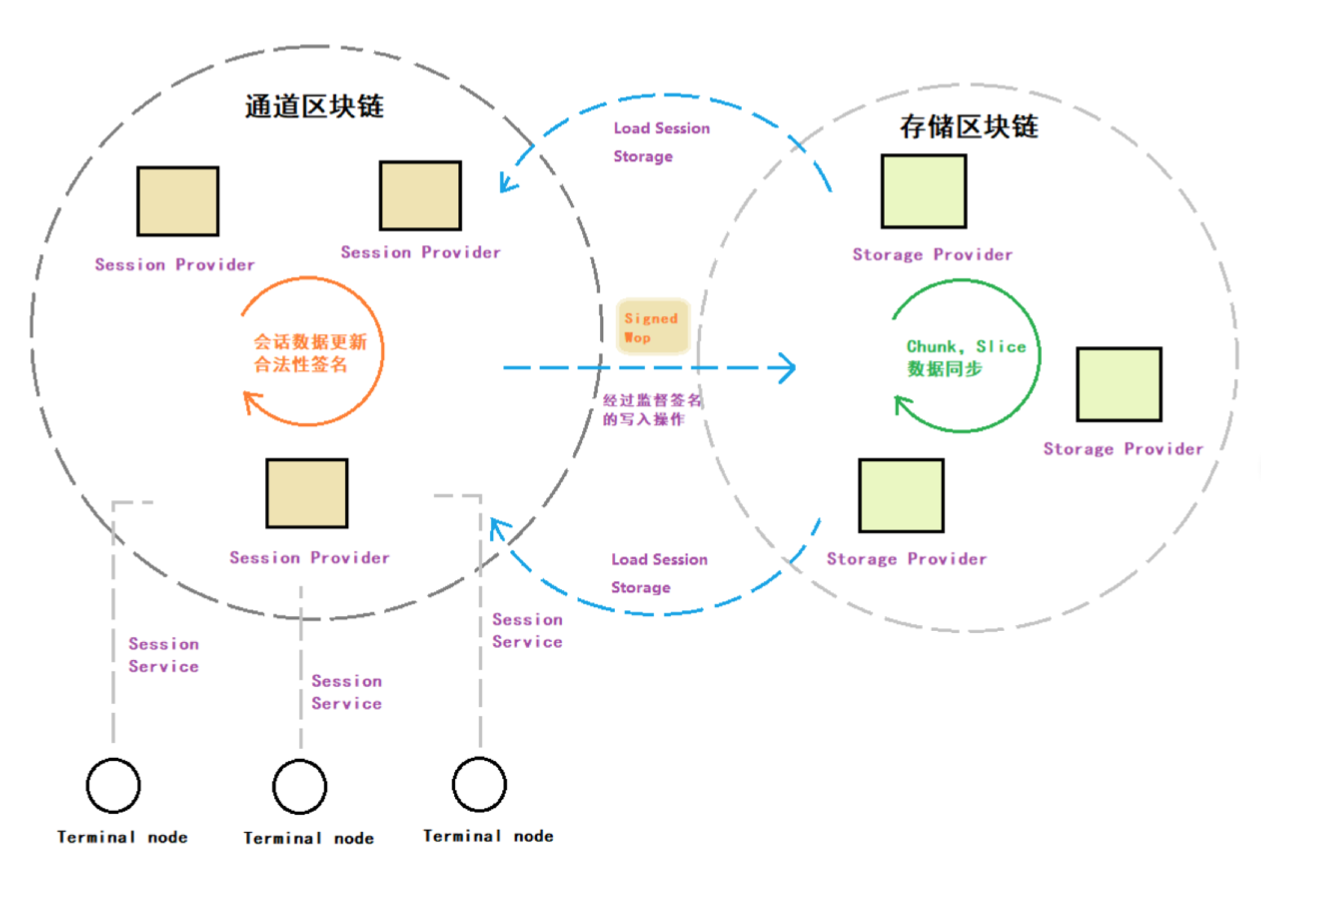
\includegraphics [width = 5in] {pic_cn/c3.png}
\caption {CNT分布式数据路由框架} \label {fig: c3}
\end {figure}

对比上图和中心化会话服务图,可以发现,CNT将中心化会话服务图中的Server和Storage分别用两个区块链取代了:
 
1.	存储区块链由高可用的分布式存储矿工节点构成,利用参与矿工提供的巨大存储空间构造高可用的存储网络;

2.	通道区块链则由高可用的分布式Relay矿工节点构成,它们主要提供动态数据路由,帮助用户根据Session参加成员构造一个所有成员都能联通的服务节点连接拓扑,以此来提供数据Relay服务,同时,参与数据Relay的服务节点能够访问存储区块链的Session Storage将会话内容不断保存起来,以便未来节点上线加载。

对于用户 Terminal node(钱包终端)来说,它得到的功能接口和体验跟中心化会话服务没有区别,而服务端利用分布式的区块链技术完全演变变成了去中心化的分布式体系。

\subsection{会话相关的存储定义}


\textbf{群组}

群组是我们日常交流的一个用户会话概念。经常通讯的一组用户,会临时或者长时间维持一个公共会话,这个公共会话体就称为一个群组,这组用户他们都称为群组成员。所有用户都退出该群组,群组才关闭,否则会一直开放。

        在区块链上维持群组的概念是分布式即时通讯的核心内容。

        一个群组中包含的元素有:

A.	参与者列表

B.	他们最近的一批聊天记录

C.	他们提供在群组中的共享文件

这组元素要求不管群组成员是否在线,它们都必须随时能够在会话建立的时候保持服务在线。这就对分布式通讯提出了存储的要求。而所有这些又都需要提供加密机制,保障内容明文不被提供服务支撑的中间节点获知。下面我们分别介绍有关会话建立,会话加密,群组成员和内容存储的相关设计。

<加图表示账户联系人空间,账户会话列表空间,会话空间>

存储区块链机制就不多介绍了,前文中描述比较多,如图所示,我们在这个巨大的存储云上切割了预定义的虚拟空间,用来提供用户的账户信息,会话信息等数据的存储,之所以预定义,是为了方便CNT的分布式通讯服务更加快捷地执行和更加便利的管理,如果这些资源都动态申请的话,在执行效率上会造成用户体验问题。
\subsection{动态路由}

	完全分布式的设计,通讯矿工节点的服务质量存在一定偶然性,它们可能任何时刻下线,或者因为处理其他事务影响服务质量,甚至连IP地址和通讯端口可能都无法保障稳定。在这种条件下,终端在请求建立一个会话服务和执行会话过程,都需要提供动态路由保障。



\subsection{会话建立过程设计}


        用户请求建立会话,该请求通过在通道区块链节点网络的广播来获取拥有服务资质的矿工节点(具体带转发跳数限制)。矿工根据Session进行分片管理,用户节点会同时向几个符合当前BlockHash的分片进行广播。矿工节点根据自己本地区块分片记录的SessionId信息推荐空闲的Session资源,并承诺自己有能力为该Session提供服务。

        用户节点收集到自荐矿工列表,从中选择能够支持同一Session分片的资源较多的矿工组,将它们的NodeId和推荐SessionId打包成一笔交易Tx{{NodeId, SessionId}}广播给该分组进行RPOW。决策矿工出矿确定最终分配的SessionId和参与会话服务的矿工节点组。

\begin {figure} [htbp]
\centering 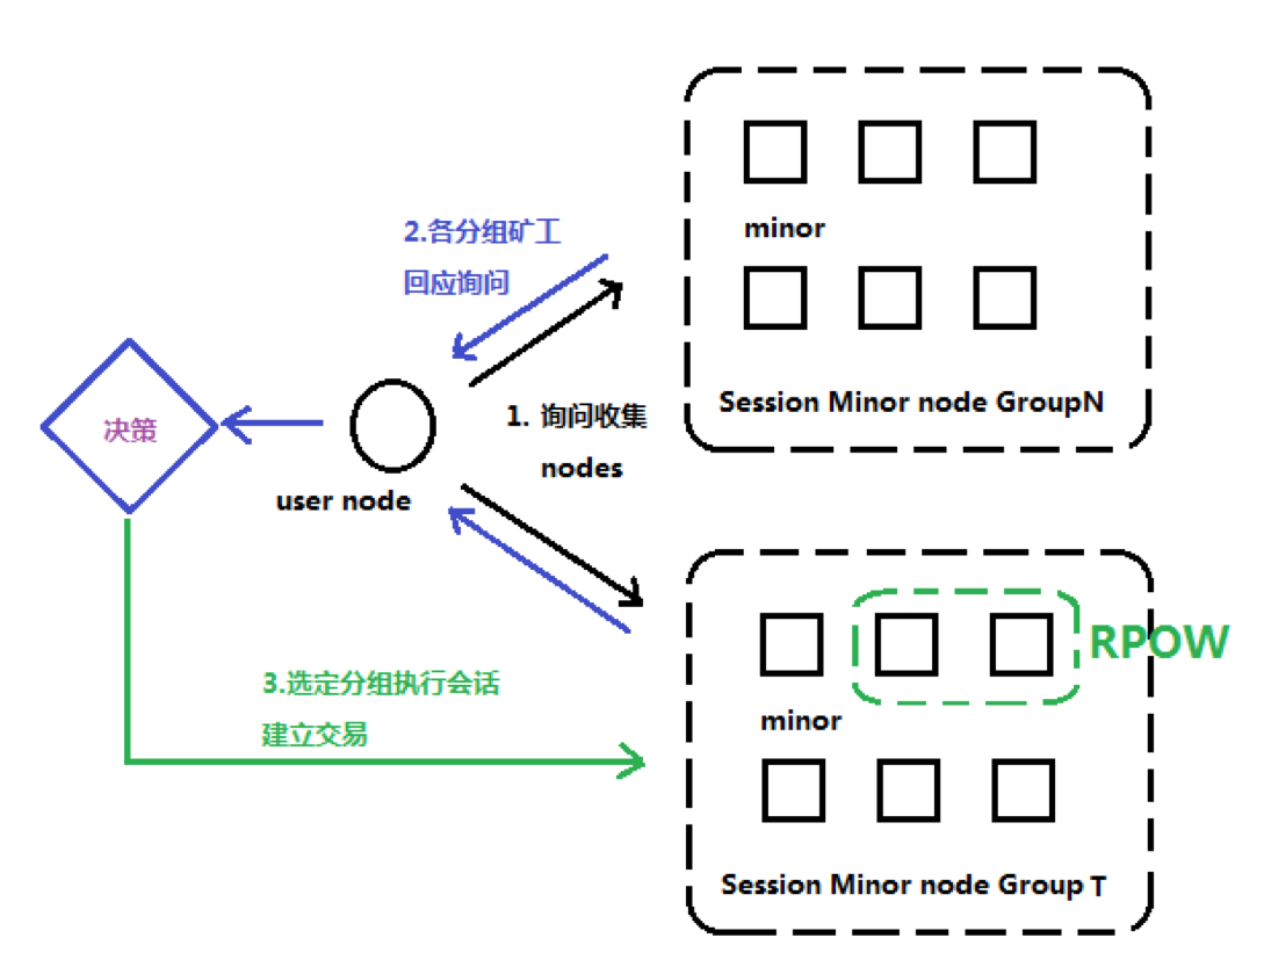
\includegraphics [width = 5in] {pic_cn/c4.png}
\caption {建立会话} \label {fig: c4}
\end {figure}

该服务节点组,根据某随机算法(比如 (NodeId\%BlockHash)\&0xff 取最小值 ),选定其中一个称为Executor node, 负责面对存储区块链的SessionId数据区域的读写操作。

从上面建立过程可以看出,建立一个会话,从申请资源到确定矿工分片,到RPOW最终同步选择,这一系列操作比较耗时,这样的步骤对于一个分布式服务而言基本是不可回避的。

为了不影响用户体验。我们可以将其中一些步骤优化处理。

为此CNT考虑在第一步选择完矿工分组后,直接选择一个评分高(自报资源多)的minor node进行沟通,如果能沟通成功则定义为本次的会话服务器(Executor node)直接开始提供Session Relay数据转发服务。Executor直接去联系交易中涉及的本组矿工列表的其他节点,同时封装一个带有所有目标用户id和服务节点列表的消息广播查找所有会话参与者,所有参与者(钱包)终端节点接到消息后,就去尝试连接各个服务节点,参加会话。

而有关构造一个交易去申请SessionId的RPOW出区块过程和连接存储区块链的过程,由Executor在后台慢慢并行完成(初次建立的会话无需从存储链读取内容,所以可以直接在服务节点内存构造)。这样对建立会话的用户体验就会有很大提升。

会话成功建立后的服务拓扑图如下:


\begin {figure} [htbp]
\centering 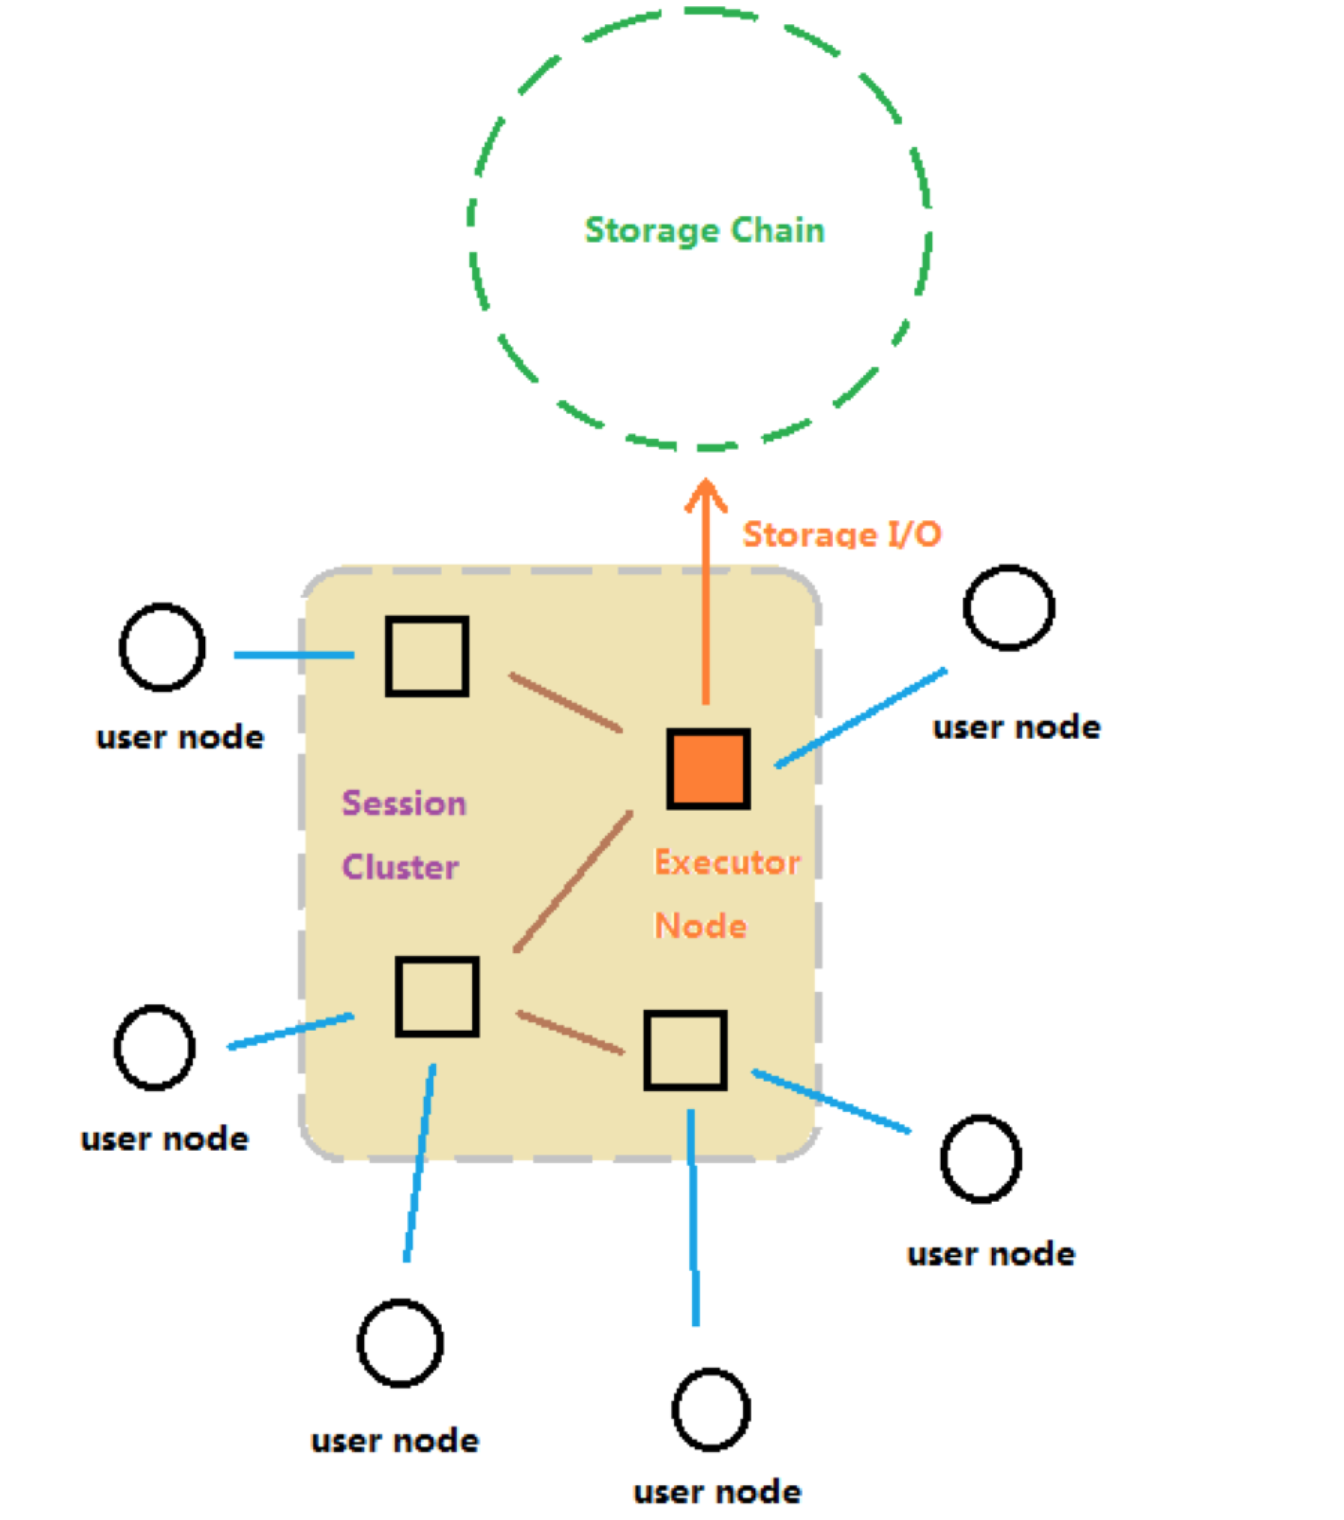
\includegraphics [width = 5in] {pic_cn/c5.png}
\caption {会话服务拓朴图} \label {fig: c5}
\end {figure}

这里有一个特殊设计:参与服务的会话服务器我们必须选择3个以上。以其中一个为主,其余的服务作为签名监督者存在。这里提出的签名监督是用来监控某种中心化职能的机制。

区块链1.0和2.0基本都是状态同步机制,所有的状态都保存在全网节点中,节点之间不涉及任何信任关系,所有的操作都要经过节点自我计算和认证形成统一共识。这样的机制足够优美和完备;而它的局限也很强烈,那就是无法实现复杂度较高,数据吞吐量较大的业务场景;这种场景以往都是由中心化服务(集群)来高效协同实现的,也是区块链应用的痛点所在。

为了实现复杂的数据存储和通信业务,CNT借助节点之间小范围校验。增加一种节点之间相互信任的机制,即让少数节点从事业务性很强的事务和数据处理,这些节点之间互相在小范围验证和相互签名,将签名结果共识给全网矿工节点。这种模型适合执行小面积影响的事务。为了防止女巫攻击,构成这个小圈子的成员尽量需要采用足够随机的进入机制,最好根据时间推移,成员构成能够随机变动,如果因为某些业务需求,无法让成员构成动态变化。则它们共同签名的事务(其他节点不知晓)获取的酬劳模型也不能是一个固定可计算(时间)和数量的模型。


\section{共识机制}
\subsection{共识机制概述}
% https://www.8btc.com/article/113137
% https://www.jianshu.com/p/b3539cd173f5

由于区块链的本质是分布式帐本,所以账本如何选择记账人、如何记账及如何同步和验证就成为核心需要解决的问题,共识机制即是指要在这些方面达成共识。目前公有链主流的共识机制是POW、POS和PBFT。

\textbf{POW}

工作量证明一开始是以工作量证明系统提出,这个概念来自Cynthia Dwork和Moni Naor在1993年发表的学术论文,是一种拒绝服务攻击和滥用服务的对策,要求发起者需要消耗一定量的计算机资源来进行计算。POW这个词在1999年由Markus Jakobsson和Ari Juels在其文章中正式提出。

比特币在Block的生成过程中使用了POW机制,一个符合要求的区块哈希需要由N个前导零构成,零的个数取决于网络的难度值。要得到合理的区块哈希需要经过大量尝试计算,计算时间取决于机器的哈希运算速度。当某个节点提供出一个合理的区块哈希值,说明该节点确实经过了大量的尝试计算,当然,并不能得出计算次数的绝对值,因为寻找合理hash是一个概率事件。当节点拥有占全网n\%的算力时,该节点即有n/100的概率找到合乎要求的区块哈希值。

%提到工作量证明,一般都会说到hash现金,亚当·贝克(Adam Back)在1997年发明的,用于抵抗邮件的拒绝服务攻击及垃圾邮件网关滥用。在比特币之前,哈希现金被用于垃圾邮件的过滤。哈希现金也被哈尔·芬尼以可重复使用的工作量证明(RPOW)的形式用于一种比特币之前的加密货币实验中。另外,戴伟的B-money、尼克·萨博的比特金(Bit-Gold)这些比特币的先行者,都是在哈希现金的框架下进行挖矿的。工作证明原理:首先工作量证明需要客户端做一个有难度的工作且得出一个结果,这个结果公布后,验证的一方需要很快能进行验证。这是不对等的。比如我们在一个字符串后加一个随机数(nonce),对这个字符串进行SHA256计算,然后得到的结果用16进制来表示,我们要求这个计算后的16进制表示的初始几位为:0000,那么才能算通过了验证。这种规则就需要计算机去不断的尝试,当然你可以记得其中一些,但是这个概率毕竟是很小的。正常情况下需要不断的输出计算尝试,直到出现正确的要求结果。

% 数学期望值,计算过程中会统计实际的计算次数,平均后得到的计算的次数,这个数学期望就是要求的“工作量”,当然这是一个符合数学统计学中的概率事件。
% POW中,算力是基础,根据算力来决定你的话语权,但是控制算力目前来看,规模越大,越无法控制甚至垄断,相对来说比较公平。
\textbf{POS 1.0}


%在POS机制中,攻击者需要拥有51\%的货币量,但是51\%的货币量被控制,这是很困难的,如果真是如此这个系统已经难以吸引到更多人使用了。
%POS的机制,那和比特币的POW机制相比,POS认为是一定程序上缩短了达成共识的时间,而且节省了资源,不像POW需要大量的算力。

%但是POS也有自己不可避免的缺点,POS类似股票,持有货币量决定话语权,前期持有币者可能占有代币比重大,就可以不断的通过利息机制获得新币,可以永久吃利息。另外,POS机制中,一旦发生了硬分叉,因为持有货币的人在两条链上都有相同数量的货币,新的分叉也能获得利益,那么这个分叉就很大程序会被默许,这样的分叉一旦出现就会不断出现,整个系统就处于崩溃,缺乏约束健壮性。

%大多数都是采用POS+POW机制,例如点点币和黑币。黑币的前5000个区块,使用纯POW机制,5001到10000使用POS和POW混合机制、10001之后采用纯POS机制。这种模式在前期完成开采和分配,然后再进入POS模式。

权益证明(POS, Proof of Stake)是由一个名叫Quantum Mechanic的数字货币爱好者在2011年在Bitcointalk论坛提出。POS合格区块可以表述为:F(Timestamp)<Target*Balance。

与POW相比,式子左边的搜索空间由Nonce变为Timestamp,Nonce值域是无限的,而Timestamp极其有限,一个合格区块的区块时间必须在前一个区块时间的规定范围之内,时间太早或者太超前的区块都不会被其他节点接纳。式子右边的目标值引入一个乘积因子余额,可见余额越大,整体目标值(Target*Balance)越大,越容易找到一个区块。因为Timestamp有限,POS铸造区块成功率主要与Balance有关。

POS只是代表一种共识机制理念,具体实现方式上有挺多可以优化的地方。目前两种比较经典的实现思路,一是Peercoin,一是Nextcoin。它们都引入了不少安全机制。

%Peercoin的设计能给POS矿工提供充足的随机性,另一方面搜索空间严格局限于Coinstake的时间戳字段,以保证影响找到合格区块链的最大因素是Kernel的币龄。

%合格区块判断条件为:

%SHA256D(nStakeModifier + txPrev.block.nTime + txPrev.offset + txPrev.nTime + txPrev.vout.n + nTime)< bnTarget * nCoinDayWeight

Peercoin是2012年8月由Scott Nadal和Sunny King提出来的。项目中,矿工需要从自己所有的UTXO中选定一个作为Kernel,构造coinstake,计算hash,如果不合格,重新构造coinstake,重构时时间戳Time会改变,也可以改变Kernel,以得到不同的Coinstake,如此往复,直到找到合格区块。Peercoin采用币龄,而不是直接采用余额(Balance)来计算。一个UTXO一旦被花费,其币天被清零,新的UTXO币龄从0开始算起。

%为了增加随机性,在POS区块中引入nStakeModifier参数,规定每隔一定时间(Modifier Interval)必须重新计算一次,取值与前一个nStakeModifier以及最新区块链哈希值有关,因此POS矿工无法提前计算,因为他不知道未来的区块哈希值。按照以上公式,如果没有参数nStakeModifier,当一个人收到一笔币得到网络确认之后,他立即就能提前计算得知自己在未来何时可以锻造区块,这显然不符合设计目标。

%权益激励,俗称获得利息,计算公式为:stakeReward = (0.01 * nCoinAge / 365) * COIN。这个公式算表明,所有的币参与挖矿,一年通胀是1\%。这被人认为是过小了。

%POS系统也存在51\%币龄攻击风险,为了增加攻击难度,Peercoin对每一笔UTXO的铸币资格做了最小年龄(stakeMinAge)限制:一个UTXO在区块链存在的时间小于stakeMinAge则没有铸币资格,PPC最小币龄为8小时。后来有些竞争币种加入了最大年龄(stakeMaxAge)限制:一个UTXO在区块链存在的时间大于stakeMaxAge则币龄始终按stakeMaxAge计算。

%Peercoin设计的POS机制中,一笔UTXO就像是一个矿工,该矿工每成功铸造一个区块后必须休息一段时间,因此,整套系统必须保证足够多的“矿工”同时在线铸造区块,才有可能获得平滑的出块速度。

Peercoin的成功运行很快就吸引了一批追随者,其中较为出名的包括新星币(Novacoin,NVC)、黑币(blackcoin,BLK)等。黑币社区认为币龄可能会被恶意的节点滥用以获得更高的网络权重并成功实施双花攻击,于是发布POS 2.0白皮书,对PPC做了几个细节优化,解决了一些潜在的安全问题,其中最重要的改进是用余额代替币龄。合格区块的条件由:F(Timastamp)<Target*币数*币的年龄,变为:F(Timastamp)<Target*币数。由于一笔UTXO无论放置多久其锻造区块的能力不变,此举可激励节点必须更多的保持在线进行铸币,提高系统安全性,将攻击途径减少到最低限度,并且能够显著提高网络保持运行的节点数量。

2013年9月,一个名为BCNext的用户在Bitcointalk论坛发起一个帖子,宣布 将发行一种全新的纯POS币种,后来取名为Nextcoin,简称NXT。NXT抛弃中本聪的UTXO设计方案,采用账户(Account)余额方案,每一个账号对应一个私钥。每一个区块都有一个生成签名(generationSignature)字段,每个矿工用自己的私钥对上一个区块的generationSignature进行签名,获得自己本区块的generationSignature,并对该字段进行SHA256运算,得hashdata,取hashdata的前8个字节该区块该矿工独一无二的hit变量。

NXT的POS实现方式与PPC完全不同,合格区块判定方法为:hit < baseTarget * effectiveBalance * elapseTime,其中baseTarget为全网难度基准值,这个难度按照每分钟一个区块目标调节,effectiveBalance为账户有效余额,elapseTime为当前时间与上一个区块时间间隔。因为hit是用户用自己的私钥签名的结果,因此对于不同用户来说具有很大随机性,即便余额很少的用户,如果运气足够好,hit值很小,也有可能快速锻造区块。

Peercoin和NXT为POS的设计打开了思路,虽然还有不足,但证明POS是行得通的。

%NXT的POS中,矿工没有搜索空间,因为当全网产生一个最新区块时,对于锻造下一个区块,每个用户自身的hit就固定了。式子右边,每个用户的目标值与自身的账户有效余额成正比关系,而且,随着时间往前推移,目标值不断变大,不等式最终一定会成立,即理论上每个节点都可以挖那个区块,但规定优先选择最早生成的区块。

%节点段造区块流程为:账户必须实时在线,当全网有最新区块产生时,每个账户立即计算自己对应的hit,然后根据公式elapseTime=hit/(baseTaret*effectiveBalance)计算得知自己锻造区块的期望时间值,并将这个期望时间广播给网络其他节点,如此,全网每个节点都知道其他节点的期望时间,从而也就得知下一个区块优先由谁来锻造。账户在自己的时间窗口锻造好区块并立即广播全网,其他节点检验一个新区块是否有效,首先要检验证区块的生成签名是否有效,还要检验新区块的时间戳是否与产生区块的节点之前发布的期望时间吻合。每次客户端检测到网络中有新的区块产生,都会重新计算自己的期望时间并向全网发布。

%对于最新区块,客户端只接受本机当前时间前后15秒范围内广播的区块,这种限制也没法体现在协议上,只能依靠客户端实时辅助实现。

%由于矿工可以将少量币转入生成的大批账号,以使每个账号每次都能产生hit,如此一来POS就有可能退化到类似POW的尴尬境地。BCNext首先从非对称签名算法下手,采用ED25519代替比特币的ECDSA,前者的计算难度比后者大。此外成熟期提高到1440个区块(1天),即一个账号有效余额一旦成功锻造一个区块,该部分余额需要等1天才能重新获得锻造资格。短暂的分叉还是不可避免的,NXT最新区块附近会有很多分支,一笔交易需要多一些确认才足够安全,NXT官方推荐10个确认。


%\textbf{POS 3.0}

%黑币社区后来进一步升级,推出POS 3.0版本,对交易手续费,难度调整做了一些优化,其中最显著的改变是将1\%年利率奖励机制变为固定数额奖励,此举不但降低代币通胀率(考虑到会有代币永久丢失,低额奖励机制回归总量恒定的设计思路),同时意味着持币节点必须实时在线才能获得收益。

\textbf{DPOS}
比特股(Bitshares)项目于2013年8月开始启动,比特股发明了一种新的共识机制——Delegated Proof Of Stake(DPOS),即股份授权股权证明。它的原理是让每一个持有比特股的人进行投票,由此产生101位代表,由它们轮流出块。持币者若想成为一名代表,需先拿自己的公钥去区块链注册,获得一个长度为32位的特有身份标识符,用户可以对这个标识符以交易的形式进行投票,得票数前101位被选为代表。代表们轮流产生区块,收益(交易手续费)平分。如果有代表不老实生产区块,很容易被其他代表和股东发现,他将立即被踢出“董事会”,空缺位置由票数排名102的代表自动填补。从某种角度来说,DPOS可以理解为多中心系统,兼具去中心化和中心化的优势。

\textbf{PBFT}

PBFT(Practical Byzantine Fault Tolerance),实用拜占庭容错算法,是由Miguel Castro和Barbara Liskov在1999年提出,可以在作恶节点少于三分之一的情况下,保证系统的正确性(避免分叉)。PBFT需要收集全部节点中超过三分之二的人的签名方可确认区块,这在大规模节点下几乎是不可行的,所以采用这一算法的必须限制节点数在少数节点,这就造成牺牲分布式的问题。一般认为与区块链最核心的特点——分布式,是背道而驰的。

为了让PBFT应用于区块链,NEO项目(delegated BFT,DBFT)是PBFT的基础上,经过一定改进后的算法。NEO主要是为共识参与节点的产生设计了一套基于持有权益比例的投票机制,通过投票决定共识参与节点(记账节点),并在在区块链中引入数字证书,解决了投票中对记账节点真实身份的认证问题。这些做法都需要中心化机构的干预,是比较中心化的做法。

%\textbf{RPCA}

%瑞波币(Ripple)的共识机制(RPCA)是是2013年提出来的,但真正应用是在2014年。RPCA每隔几秒就可以维持整个网络的有效性和一致性,这是十分高效的。在瑞波币共识证明算法中,节点能够人为的干涉投票和维持可信节点列表,这是比较中心化的设计,可以人工维护节点,但也有改动节点的风险。RPCA的缺点就是易于遭受攻击,黑客可以伪造node,甚至可以大量扩散潜伏,并在某个时间突然攻击所有网络。自然它可以采用手工干预,剔除网络中不安全节点。但问题在于中心化维护人员也可能作恶。瑞波的共识机制是联盟链的做法,并非公有链的选项。

\textbf{BFT-DPOS}

%在传统DPoS共识机制中,我们让每个见证人在出块时向全网广播这个区块,但即使其他见证人收到了目前的新区块,也无法对新区块进行确认,需要等待轮到自己出块时,才能通过生产区块来确认之前的区块。见证人出块时向全网广播,其他见证人收到新区块后,立即对此区块进行验证,并将验证签名完成的区块立即返回出块见证人,不需等待其他见证人自己出块时再确认。

%出块见证人生产了一个区块,并全网广播,然后陆续收到了其他见证人对此区块的确认,在收到2/3见证人确认的瞬间,区块(包括其中的交易)就不可逆了。交易确认时间大大缩短,从45秒缩短至3秒左右(主要为等待生产区块的时间)。

2017年出现的EOS将BFT和DPOS结合起来,先选出21个超级节点(主力见证人节点)及100个备选见证人节点,将原先的随机出块顺序改为由见证人商议后确定的出块顺序,这样网络连接延迟较低的见证人之间就可以相邻出块。当21个主力见证人的15个确认交易后,交易即不可逆转。按EOS的设计0.5秒就可以出块,1秒就可以全网确认。每个见证人连续生产6个区块,也就是每个见证人还是负责3秒的区块生产,但是由最初的只生产1个变成生产6个。%最恶劣的情况下,6个区块中,最后一个或两个有可能因为网络延迟或其他意外被下一个见证人略过,但6个区块中的前几个会有足够的时间传递给下一个见证人。

每个区块生产后立即进行全网广播,区块生产者一边等待0.5秒生产下一个区块,同时会接收其他见证人对于上一个区块的确认结果。新区块的生产和旧区块确认的接收同时进行。大部分的情况下,交易会在1秒之内确认(不可逆)。这其中包括了0.5秒的区块生产,和要求其他见证人确认的时间。

%分叉问题:所有节点都不会自动转移到分叉链上,因为分叉链上没有区块生产者可以满足上面所说的15/21法则。即使多数见证人想分叉区块链,也只能以相同的速度(0.5秒)与主链竞争,就算主链只剩下一个见证人,分叉链也永远不会追上主链,保证了系统的稳定。

BFT-DPOS共识机制极大的提高了出块的效率,但也有致命的缺点,它不是完全去中心化,可能会有多个中心之间共同串通而损害整个社区利益的行为。另外,它依赖于投票机制,而投票制度其实有以下问题:首先,有可能最后投票的参与度会很低,影响投票结果;其次,也会可能有这种情况,例如用户把币都存在了交易所,交易所有可能会代替他们去投票,但是用户并不是很在意到底交易所会把票投向何处,这可能造成交易所作恶的情况发生。总之,这一方式类似联盟链,与公有链对分布式的追求是背道而驰的。

\textbf{Casper}

% github上capser地址:https://github.com/ethereum/casper

以太坊的POW效率虽然比比特币要高,也有一定的抗专用矿机的机制,但其TPS平均不一20笔,为了提高效率,以太坊的开发者Vlad Zamfir\cite{VladZamfir}提出了一种新的POS机制,即Casper,它类似于Tendermint。虽然Casper可能要到2020年才能落地,但其提出来的基于保证金的经济激励共识协议(security-deposit based economic consensus protocol),值得探讨。

Casper协议中的节点,作为“锁定保证金的验证人(bonded validators)”,必须先缴纳保证金(这一步叫做锁定保证金,"bonding")才可以参与出块和共识形成。Casper共识协议通过对这些保证金的直接控制来约束验证人的行为。具体来说就是,如果一个验证人作出了任何Casper认为“无效”的事情,他的保证金将被罚没,出块和参与共识的权利也会被取消。保证金的引入解决了"nothing at stake",也就是经典POS协议中做坏事的代价很低的问题。现在有了代价,而且被客观证明做错事的验证人将会付出这个代价。

Casper的共识称为下注共识 (Gambling on Consensus)。Casper要求验证人将保证金中的大部分对共识结果进行下注。而共识结果又通过验证人的下注情况形成:验证人必须猜测其他人会赌哪个块胜出,同时也下注这个块。如果赌对了,他们就可以拿回保证金外加交易费用,可能还会有一些新发的货币;如果下注没有迅速达成一致,他们只能拿回部分保证金。因此数个回合之后验证人的下注分布就会收敛。

Casper中的区块需要锁定保证金的验证人中的绝大多数达到67\%到90\%的验证人下注这一区块时并且概率达到99\%以上才能进行确认。如果达不成共识就需要多轮下注。当所有小于高度H的块都已最终确认,就可以说这个H-1高度的状态已最终确认。

%防审查(Censorship Resistance):共识协议最大的威胁之一是矿工形成以损害非成员利益为代价最大化成员获利的联盟。如果Casper中验证人的收入主要由手续费构成,一个多数联盟就能够通过过滤其它节点的出块来获取更大利益。不仅如此,攻击者还可以贿赂节点来剔除特定地址发出的交易,只要多数节点是理性的,他们就能够联合起来过滤掉没有剔除指定交易的块。

为了抵御多数派联盟攻击,Casper需要设计一套合作博弈机制,确保每一个节点只有在由所有节点组成的联盟中才能获得最大利益,即如果p\%的验证人参与了共识博弈,那么他们将得到f(p) ≤ p\%的收益,而如果有100\%的验证人参与则能获得更多回报。而这一设计是Casper的难点。


\subsubsection{优劣总结}

通过以上分析可知,BFT主要适合于联盟链或者对其它共识机制作补充,公有链的主要选择应该是POW和POS。从长远看,特别是从区块链应用于生活的各个方面看,POW并不合理,再改进的空间也很小了,而POS通过不断的改进将成为公有链的主流。以下分别从去中心化、能耗、安全性、共识速度、交易容量、出卖平滑度、贫富差距、最终性等对POW和POS进行比较。

去中心化。POW使拥有算力的就有可能获得记账机会,其设计之初希望能够做到最大限度的去中心化,但针对特定哈希算法的专门芯片的出现改变了这一格局,它使一般电脑难以参与记账竞争,而矿池的出现进一步影响了分布式的拓扑结构,它使即使是专用矿机,做SOLO挖矿也几乎不可能了。所以POW在硬件去中心化上并不是很充分的。POS使只要持有代币就有可能获得记账机会,而持有越多机会越大,通过一定的设计也可以增加随机性,以使去中心化得以提高。

安全性。POW最大的优点是安全性。首先其安全性存在完整的数学证明,这一点是POS和DPOS无可比拟的优势。区块链共识机制一般要同时考虑抵御DDOS攻击和双重支付攻击,POW存在51\%算力攻击威胁,比特币目前超强的算力使得破坏该系统需付出巨大代价。但是,对于一个新项目,使用POW可能是非常危险的,因为现在的算力可能租用于进行攻击,对于新项目反而POS更加安全。NXT项目理论上可以实现快速交易,但需要锻造节点曝光自己的IP,如此一来容易成为DDOS攻击对象,DPOS的代表也容易成为DDOS攻击对象。虽然POS也会存在51\%币龄攻击,而DPOS安全性完全取决于代表的诚实程度,但并非不能设计的,Casper的抵押机会就可以增加做恶成本。

能耗。POW不仅能耗惊人,也需要投入大量的CPU和外设,浪费是很大的,而POS没有这方面的问题。

共识速度。POW很难缩短区块时间,POS相对而言可以缩短区块时间,尤其NXT会比PPC的实现方式更快,DPOS也可以在很短时间内达成共识,比特股目前30秒产生一个区块。不过POS更容易产生分叉,尤其NXT,所以交易需要等更多确认才被认为安全。

交易容量。这是区块链未来发展需要解决的核心问题,巨大的交易容易意味着巨大的带宽和存储空间,POW的交易容量很难扩展,而NXT由于每个节点都可以预知下一个区块由谁锻造,可以直接将交易发给锻造节点,因此NXT交易容量有很大扩展性。从某种角度来说,DPOS可以理解为多中心系统,兼具去中心化和中心化的优点,如果代表节点都运行强大的服务器且彼此带宽足够大,理论上交易处理能力可比拟传统中心化系统,比如Visa。

出块平滑度。POW由于哈希算法特性,可以得到平滑出块速度,而且可以间隔一段时间再调整全网难度,POS出块主要与余额有关,而用户余额差距梯度比较大,所以POS一般每个块都要调整全网基础难度。DPOS依靠有限代表人的协同作用,如果代表人不会频繁进出,几乎可以做到固定死出块间距。

贫富差距。POS使持有币越多机会越大,赚得越多,而机会更加增大,这样就会拉大贫富差距,使囤币就可以产生收益。这被认为POW优于POS的重要一点,但其实POW也是越富的会囤更多机器,并赚更多币,就这一点看,POW与POW一样,投入越多得到机会越大,但POW投入的资源是用于做哈希碰撞,而POS投资的资源是买币,所以POS在这方面反而更胜一筹。

最终性。POW通过竞争达成共识,不存在最终性,理论上如果有足够算力,现在可以从头挖比特币区块链,不过可以依靠检测点实现最终性。NXT和DPOS严格依赖时间轴,依靠节点实时在线检测,所以存在最终性。

无抵押(nothing at stake)问题。Casper解决了无抵押的问题,使作恶成本提高了。但大部分现在的机制还存在这一问题。

综合各方优势,在去中心化、安全、效率和能耗等不能同时兼备时,POW彻底抛弃节约能源的需求,通过巨大算力来维护系统安全和去中心化特征。POS几乎不费多余电力,但需要在另外两个特性做出牺牲。POW被证明为了安全和去中心在能耗和效率上做出过大的牺牲,特别是当需要把区块链应用于社会生活各个方成时,POW几乎不可行。一个区块链系统的设计本来就需要对去中心化、安全、效率、能耗等各方面进行平衡,而不是只追求一方面的性能,但POW的特点是,一旦开了一个POW的口子,就可能造成算力大战,这使POW的改造空间很小了。POS在设计上有更多空间,能够通过设计平衡各方面的性能,更加适应用于公链系统。另外,Casper代表了POS最新成就,可以在其基础上进行设计。

\subsection{CNT的POS机制}

\subsubsection{CNT对POS设计上的需求}

以上分析可知,POS相对于POW有很多优点,CNT应该选择POS作为共识机制,但在设计上需要根据不同公有链的诉求对各方面性能进行平衡。那么CNT的需求按重要性,有哪些呢?

排在第一位的是分布式。CNT的目标是要促进人类的交流和交易,使人类以最小的颗粒进行合作,这就要求任何个人、组织、智能程序都可以加入提供资源或成为用户,它们能够突破国家、制度、种族等进行合作,只有足够分布式的系统才能做到最低的进入和退出门槛。

排在第二位的是安全性。只有做到足够的安全性,系统才能够长期运行。安全性包括两类:一类是重大安全,是指影响是全局的,一旦出现,系统就面临崩溃,这是必须避免的;另一类是次要安全,是指出现后,系统能够继续运行,影响是局部的。系统设计上,要杜绝重大风险,尽量排除次要风险,设计系统风险出现后的恢复机制。恢复机制在中心化系统中是比较容易设计出方案的,但分布式系统中如何恢复,设计上比较困难,一般需要通过社区行为和经济博弈自动出现。

排在第三位的是效率,包括共识速度、交易容量、出块平滑度等。由于交易容量受到网络宽带的限制,重点需要设计的是共识速度和出卖平滑。交易容量的扩大在互联网宽带一定的情况下只能通过分片进行,这将在“分片机制”一章中专门介绍。

排在第四位的是要避免不公。在设计上避免不劳而获和付出没有收获的情况,另外,付出与收益上要进行平衡。

排在第五位的资源消耗,包括设备和能耗。排除了POW就使资源消耗得到了极大的控制,在POS的设计上,要避免过大的搜索空间以及POS退化化POW。

根据以上要求,CNT在POS的设计上具有有以下特点:

\begin{itemize}
\item 在分布式方面,将让任何愿意参与者都有获得贡献资源的机会。在出块上任何参考者达到容易达到的最基本的条件就有可能获得出块机会。
\item 在效率方面,将在某段时间集中在某些节点出块,并在一段时间后重新决定出块名单。
\item 在安全性方面,将对可能出现女巫攻击、51\%攻击、DDoS攻击等做出专门的设计。
\end{itemize}

另外,一个良好运行的共识还需要在以下方面进行优化。

\textbf{随机性}

要使所有参与者都有可能获得出块机会,同时,由于对等网络上的每个矿工都可能选择一个对自己有利的结果,从而操纵下一步出块,就需要引入一定的随机性。

引入随机机制还必须达成共识,这就是对等网络上引入随机机制的困难。同时,还有另一个困难,整个主网都是依赖于算法的话,其实已经很难有随机性了,所谓通过计算本身产生的随机都是伪随机的,是有可能被破解的。

工作量证明是通过哈希计算完成随机性的。权益证明许诺能够以更低的成本选出记账人,但随机性需要专门的设计。它可能是一个类似Peercoin的搜索空间,或者Nextcoin与每个矿工的私钥相关。

我们发现通过引入一个非工作量证明的随机数是很难达成共识的,而计算生成的随机数是伪随机的。如果引入大自然的随机数是可能的,但这就需要一个收集随机数并发送随机数的机制,这用非中心化的方法是很难达到的。

我们唯一能选择的是人这样的带随机性的动物,通过他们博弈结果的不确定性来获得随机性。由于每个矿工节点操纵者背后实际操作者是人,所以设计出一个带随机性的集体决策来就可能达成目标。

\textbf{收敛性}

收敛性是指最终能够选择出记账人。

\textbf{利益相关性}

如果一个系统的出块者没有抵押物,其攻击成本将减少。

\textbf{最终性}

如果有足够的资源从头开始挖一条链,会得到一条更长的链,并使其它矿工认为该链是合法的,就可以进行长程攻击,而这样的链就缺乏最终性。

\textbf{客观性(Subjectivity)}

共识机制的一个目标是要让新进入者通过从对等节点收到的信息评估对等网络系统的现状。这一特性在抗女巫攻击时比较重。

客观性是指新进入者能够独立地以协议规则(比如,对创世区块的定义)和全网广播的信息获知与网络其它节点对系统现状的同样的认知。

POW是一个客观性的例子,只要节点连接到至少一个“诚实节点”,它就可以选择一个有效的区块链,这是因为这条链拥有最大的累积诸难度。

与PoW不同,权益证明不是客观的,只能通过增加人的随机性以达到弱客观性(Weak Subjectivity)。假如一个节点除了协议规则(比如,对创世区块的定义)和全网广播的信息以外还需要最近状态的信息才能对系统现状进行判断,那这样的共识机制就是弱客观性的。

弱客观性虽然因为引入人的随机性牺牲了去中心化和数学上的完备性,但它在结合计算机驱动和社会驱动上是比较好的方法\citep{VB_PoS}。

\subsubsection{防止可能的攻击}

基于安全性的重要,良好的系统应该能够防止各种攻击,这部分专门论述需要重点防范的攻击。

\textbf{防止女巫攻击}

女巫攻击是任何对等网络系统难以完全避免的,所能做的是提高其攻击难度。POS通过使用时间、随机性、押金等机制可以防止女巫攻击。

\textbf{防止DDos攻击}

如果可以预测下一个或几个出块者,只要对期实施DDoS攻击就可以使系统瘫痪。通过引入随机性、收费机制可以有效防止DDoS攻击。


\textbf{预挖双花攻击}

双花攻击要求攻击者在支出一笔钱后,私下准备一条比较长的链私挖,并在对方\footnote{这类双花需要准备一大笔钱,还需要有地方愿意接受。一般是交易所愿意接受一大笔资金,通过交易所也容易变现脱手。}确认收到资金后把私挖的链发布出来,在私挖的链上这笔资金是转到了另一个地方。


\textbf{贿赂双花攻击(Bribe Attack)}

攻击者为了让矿工放弃现有的链而使用自己准备的链,只要提供更大的收益,从而实现双花。

如果攻击失败,攻击者并不会失去什么,只要自己的贿赂小于双花收入就有利可图。

\textbf{币龄积累双花攻击}

针对Peercoin或其它使用币龄为基础而不是以财富为基础的共识机制,从理论上说,只要等待足够长时间,攻击者可能积累足够多的币龄以颠覆系统。

如果掌握Peercoin的未花输出(UTXOs)5\%币,分成不同的输出,等待其币龄是其它币的10倍,就有可能实现双花攻击。所以在Peercoin后来的版本以及黑币(BlackCoin)中,币龄会乘一个权重,币龄越大越打折越大。

\textbf{长程攻击(Long Range Attack)}

Nxt系统中,超过720个块的链将不被系统接受,在该系统中约12个小时。但这一方面对于新加入者比较难实现,因为没有历史知识作为比较。


\subsubsection{CNT的共识机制}

\textbf{选择Casper为基础框架的原因}

共识机制没有绝对的好坏,关键是要能满足经济模型提出的需求。CNT要求分布式水平、安全和效率上的平衡,目前的共识机制Casper是最符合的选择。

首先,在分布式方面,Casper的验证人数量上百,非常难串谋,而验证人的加入和退出不需要人为干预,可以做到足够的分布式。

其次,在效率方面,Casper缩小了共识的范围,比较容易通过定向广播来减少网络负担。

最后,安全性方面,Casper有以下几个优点:
\begin{enumerate}
\item 通过灯塔主链随机选择验证人分配到各分片,能够使各分片的安全与全网安全一致。
\item 押金机制增加了攻击的难度。
\item 引入了众多个人,这些个人的组合形成比较大的随机性,让各种攻击变得困难。
\end{enumerate}

\textbf{PoW+Casper+PBFT}

CNT的共识机制,在主链上使用类似现在以太坊的PoW机制,以保障安全和随机性,在分片上采用PBFT机制,以保障出块,而为了保障分片上PBFT的安全性,将使用Casper的机制预选出块人池子,并利用PoW定期轮换各分片的出块人。

通过增加进入PBFT矿工池子的难度和退出难度,并增加选择的随机性,将很难通过女巫攻击对分片造成伤害。

下图是CNT的共识机制的架构:

\begin {figure} [htbp]
\centering 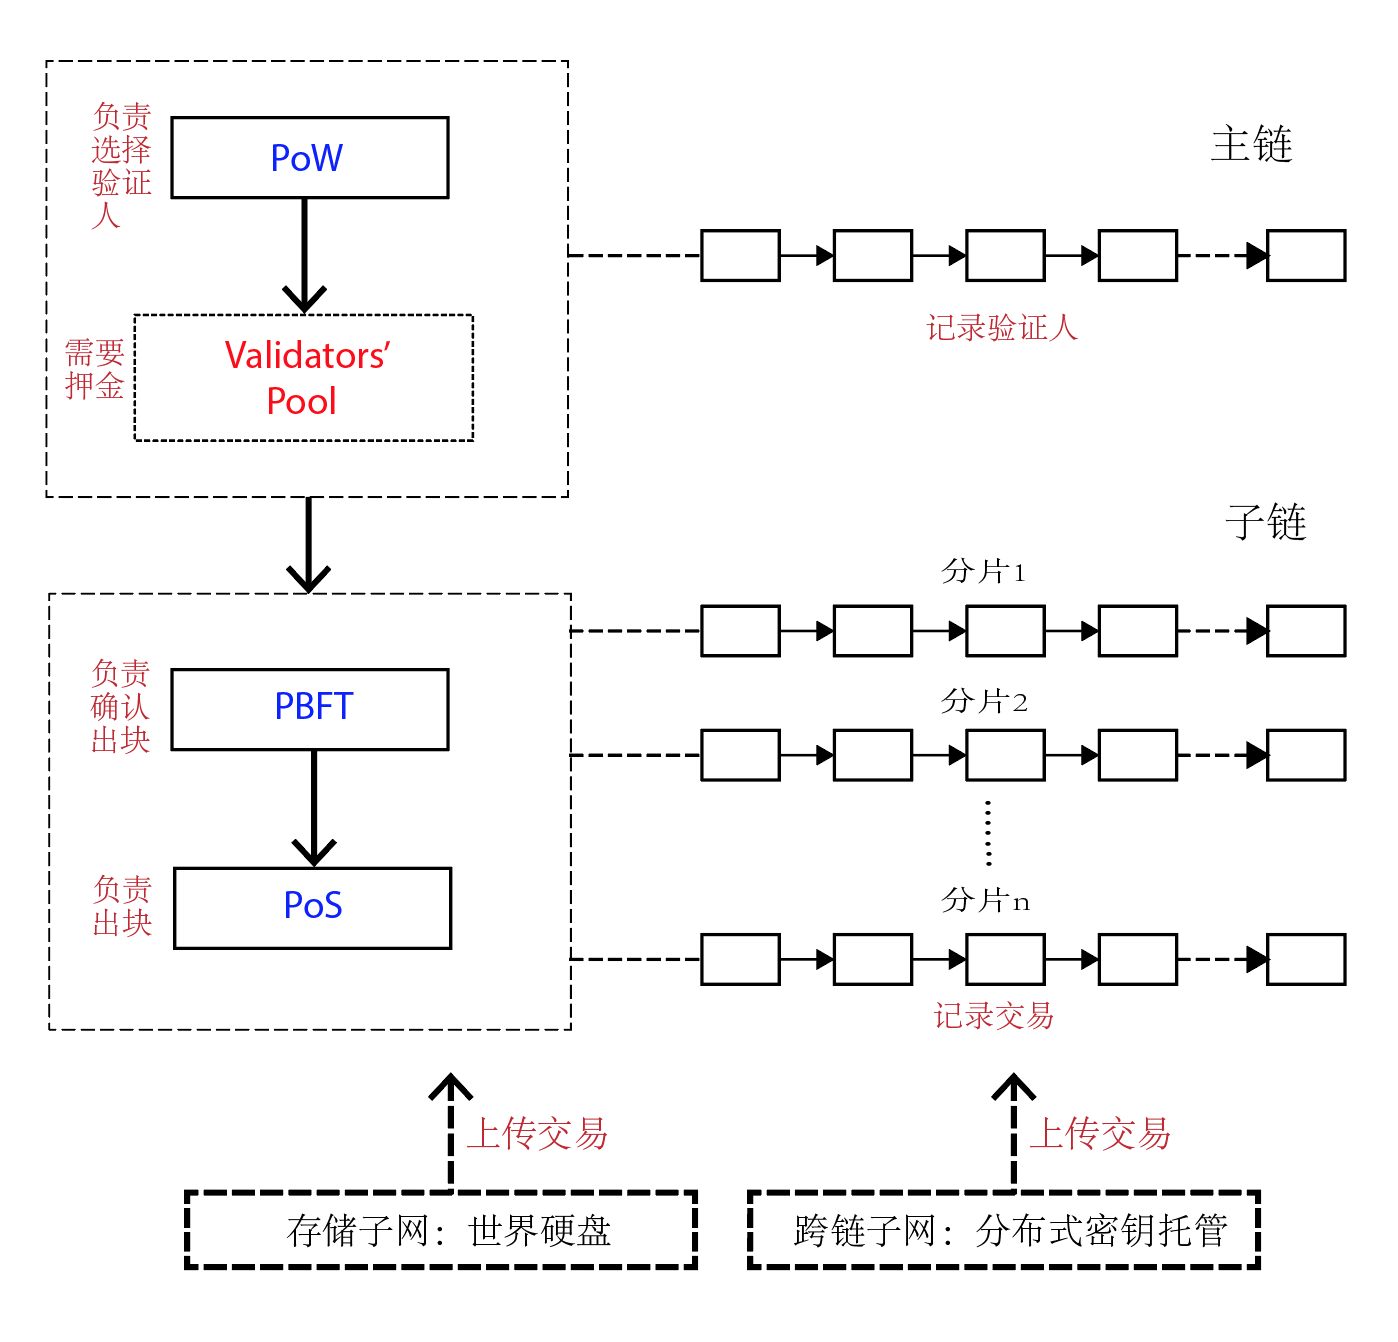
\includegraphics [width = 4in] {pic_cn/consensus.png}
\caption {CNT共识机制} \label {fig: consensus}
\end {figure}


%\textbf{POS的验证人机制}

%\subsubsection{出块条件}
%\subsubsection{出块效率}



\section{分片机制}
\subsection{分片概述}
% https://blockonomi.com/sharding/
\subsubsection{扩容概述}

区块链的交易效率要达到实用的级别就需要TPS达到一万笔每秒。这实际上是一个刚需。目前比特币是每秒5到10笔,以太坊是10到20笔。就算以太坊升级到权益证明,其TPS也很难突破500笔。区块链需要的是从现在10笔扩展一千倍的方案。

单个链的结构是很难达到每秒一万的这个数量级的,这主要是因为宽带限制造成的。因为每秒一万笔的交易包必须及时的同步到全网,不然就会造成大量的软叉,使系统趋于崩溃。随着单链规模越大,即分布式越强,同步效率越低,TPS越低。

比特币的努力还是建立在单链基础上的:

\begin{itemize}
\item 目前,最主要的努力是增加块大小。从1M向上扩展,例如比特币现金分叉,从1M扩展到8M也只是扩大了8倍。增加8倍而在其它方面并没有什么提升,其应用场景也只能是大额转账,这对于原始比特币来说算力和大家的认可才是关键因素,所以分叉币者没能超过原始比特币。
\item 或者通过减少出块时间,这期与增加块大小是类似的做法,因为区块数据总是要全网广播的,不论是增加块大小还是减少出块时间,都会遇到同步效率的瓶颈。莱特币正是将时间从10分钟减少到2.5分钟,但这样的速度提升是有限的。
\item 隔离验证(SegWit)虽然可能减少同样数量交易的广播量,但这种技术革新对扩容的帮助是很有限的。
\item 最后,线下扩容方案,类似闪电网络这样的侧链,并不能算在区块链的交易效率里,因为它是一种使用场景很有限的方案。
\end{itemize}

NEO使用了dBFT共识机制,但其对效率的提升是有限的。IOTA使用了DAG技术,它已经不是区块链,很难防止双花。相较而言,以太坊的努力可能更加合理。它选择了共识机制从工作量证明转为权益证明,把单链机制通过分片转化为多片机制。目前两者的升级准备放在一起升级,最早要到2019年下半年。

总结而言,本项目最好的选择是在以太坊的基础上进行技术迭代。

\subsubsection{以太坊分片概述}

分片(Sharding)要比区块链技术要先出现得多,广泛用在商业数据最优化到谷歌全球关系型数据库中。分片最主要的乃就是用一些特殊的方法将数据在一个数据库中进行平行拆分。一般来说,这些分拆出来的数据被称为分片(Shards)。

在区块链分布式网络中,网络由一系列按一定方式相互关联的对等网络节点构成。目前来看,每个节点都存储了该网络和交易的所有数据,这就会在可扩展性方面造成严重的问题。

以太坊存储了区块链所有数据,包括帐户余额、存储和合约代码。整个系统的限制来源于节点之间形成共识的通讯瓶颈。由于每个节点都没有特权,整个网络节点的速度只和单个节点一样快。

以太坊的分片的想法,并非对数据进行分片而是对节点进行分组,从而通过平行处理数据解除系统的可扩展性瓶颈,从而极大的提高交易性能。以太坊甚至认为可以通过让每个分片都有自己的特点,而分片之间通过某种协议进行通讯。

以太坊将所有交易及智能合约进行分组,每个分组将拥有数据头和数据主体。数据主体是所有的该组的交易。数据头包括:

\begin{itemize}
\item 分片号;
\item 随机取样(random sampling),将验证者分片;
\item 分片梅克尔根。
\end{itemize}

所有的交易都发生在分片内的帐户间,分片内的共识机制是权益证明。以太坊每个区块将包括全局状态根和交易组的根,前者为所有后者的梅克尔根。

为了避免通过单个分片攻击其它分片,随机取样产生验证者是跨分片的,这样攻击者由于不确定验证者将分到哪个分片,因此攻击者难以实行跨片攻击。

以太坊这一设计的难点是跨片通讯协议,它的设计非常复杂,成本也高,所以只在必需的时候使用。当一个节点要请求的信息并不保存在本分片时,就需要使用跨片通讯(cross-shard communication)。

跨片通讯是通过交易收据(transaction receipts)实现的。交易收据保存在梅克尔根,所以容易被验证,但并不数据状态根(the state root)一一部分。当一个分片收到另一个分片的交易时,它将检查梅克尔根以确保收据是没有花销过的。收据是保存在共享的内存,它可以被其它分片验证,但不被修改。因此通过,分布式保存的收据,分片可以相互交流。

以太坊分片做法是包含主链和子链,主链负责管理验证者,子链负责交易,子链包含100个子链,账户交易信息都是储存在子链上的。具体做法如下:
\begin{enumerate}
\item 参与主链:即存款到权益池,向Casper帐户发送32个ETH的存款,附带一个公钥和一个取款地址。等待一天时间,协议会将这笔交易信息纳入验证者池。
\item 主链的工作:追踪子链上的区块,将验证者随机分配到分片,并追踪验证节点的信息,包括分配到什么分片、有没有奖励和惩罚。
\item 验证节点的工作:主链出块;验证主链上的出块、交易以及对验证节点的奖励和罚款;验证及确认分片间交易;分片出块。
\item 奖励:在线正常运行的状况发出了应该发出的信息,所有都是正常的,这种情况下会发现其他的三分之二节点正常,就可以拿到利息。
\item 惩罚:不过至少有三分之二的节点都在正常运行,会有一些小的惩罚。但是,如果大部分节点离线,那么,会有大的惩罚。最差的情况是,签名是错误或者跟自己有冲突的信息,这可能是你要攻击网络,或者你被黑了,如果有这样的情况发生,你会有一些惩罚。这个惩罚与其它犯错验证节点的数量是成比例的,因为攻击需要多个节点同时参与。攻击系统的成本非常高,如果你作为个人的验证节点出现了问题,成本是没有那么高的,是公正的。这个机制希望激励大家做验证节点,也希望大家在设置时,能够更好的保护自己的机制,尽量不与其它节点的安全保护同时失败。
\item 退出主链:即取款,私钥或提款地址都可以触发取款过程,一旦触发,你的验证节点会在大概7天后关闭,你退出了之后,需要等待4个月,来提取以太币。
\end{enumerate}

以太坊的Casper升级要推迟到2019年下半年,而分片可能要2020年到2021年。由于Casper升级本身有难度,因为从PoW转到PoS需要一个较长的过渡时间,不然很多PoW矿工会受到较大影响,所以以太坊的分片实现可能需要等待较长的时间。

\subsubsection{其它分片概述}
%https://docs.zilliqa.com/whitepaper.pdf
其它项目采用分片的比较有名的是Zilliqa,它目前不实现状态分片,只进行交易和计算的分片。它声称可以达到数千的交易量。

它在每个分片使用PBFT共识机制。原因是POS的最重性没有PBFT高。Zilliqa在较长的时间间隔,需要投票时使用了POW。%没有图灵完备的智能合约。

由于每个分片进行交易计算形成小区块,然后这些区块再合并成一个大区块,所以它的状态并没有分格。这样的做法,难以应对区块链可扩展性瓶颈。

\subsubsection{分片的难点}

所以多条链平行是一个必然的设计。但也提出以下问题:

\begin{enumerate}
\item 如何使数据主要保存在单片里,不用全部广播到多片,不然失去了分片的主要意义。
\item 在数据主要在单片的情况下,如何原生代币在全网得到一致认同。
\item 如何进行片间交易。
\item 如何在多片间平衡负载。
\item 如何避免从一个片发起对全网的攻击。
\end{enumerate}

讨论分片不能不讨论三角悖论。分布式、安全和效率构成了不可能三角,需要对三者进行平衡。但是在公有链的情况下,随着节点数增加效率并没有提高,同步却更难了。一万台机器产生共谋的可能并不比一千台机器多多少,一味坚持分布式是不合理的。所以,随着节点数的增加,将一条链分裂成多个片的设计是合理的。

分片包括三个方面,一是计算的分片,二是数据的分片,三是交易的分片。智能合约分布在不同的片,可以节约计算资源,而数据放在不同的分片可以节约宽带资源,交易放在不同的分片则可以。

\subsection{CNT的分片和分裂机制}

CNT采用片内独立出块,片间交易通过主链中转的方式进行分片。为了片间交易的安全,跨片交易将引入“警察机制”,对数据进行核定。

CNT做到了交易、数据和计算的分片。每个分片即是独立的,又相互承认对方链上的数据,并可以发起跨片交易。

分片会自动升级,即分裂机制。当节点达到一定数量时,子链将进行分裂,从而形成多个分片。分裂的机制要考虑一定的随机性。分裂之后的数据将与分裂前产生继承关系。

\subsection{智能合约}

CNT是基于以太坊的go语言版本开发的,将拥有并兼容以太坊合约的各种功能,并将扩展其功能使其拥有数据读写和通讯的功能。

这样的智能合约将拥有先知的功能,即可以从外部读入数据,并且可以发出各种Email,以触发通知。

智能合约将在分片中进行,也可以发起片间交易。


\section{区块链社会、数据服务商与应用场景}

\subsection{从图灵完备到功能完备:将区块链应用于社会各方面}
根据区块链科学研究所创始人梅兰妮·斯万的观点,区块链技术发展分为三个阶段:1.0为可编程货币、2.0为可编程金融、3.0为可编程社会。比特币及各种竞争币是属于区块链1.0。以太坊因为是图灵完备的有定程序上实际了区块链2.0。但是,由于以太坊存储、跨链、通讯等功能,它并不是功能完备的,也难以用于很多方面。现有的其它区块链由于没有同时具备完全分布式、无限可扩展、通讯、存储、跨链等功能,也很难应用于社会的方方面面,这也是为什么我们现在还没有看到重要的App被DApp替代的原因。

Contatract是完全分布式和无限可扩展的,并且拥有通讯、存储、跨链等功能,这就是CNT拥有了可以应用于社会各方面的能力,是真正的区块链3.0项目。Contatract几乎可以应用于任何场景,以下仅列举少数应用场景加以说明。

\subsection{数据服务商}

数据服务商实际上是DApp创业者,用户的大部分数据他们自己并不拥有,他们所做的是收集数据标签和说明,将其进行分析,做数据挖掘和数据推送等服务。
  
\subsection{区块链搜索}

大师的数据将积累在分布式存储系统中,对这些数据进行探索就变成一个重要的工作。区块链搜索是指对分布式存储上所有对外开放的数据的搜索。

\subsection{分布式云存储服务}
CNT的存储子链构成一块大的“世界硬盘”,能够无限可扩展,并为个人和企业提供分布式的云存储服务,使用者还可以随时生成哈希上传,以证明不可篡改,可以成为分布式的Dropbox。特别是对于企业,对数据安全和隐私保护有更大的需求,CNT的大象存储对于他们有很可的吸引力。

\subsection{分布式通讯和在线直播}
CNT赋予地址之间地址通讯的能力,实际上是一个分布式通讯的工具,通讯数据不会被除会话之外的任何人审核或掌握,可能成为分布式的微信并提供各类在线直播服务。由于区块链支付的方便性,在会话中很容易进行打赏。

\subsection{区块链身份服务}
地址可以在自己的空间上传自己的身份信息,包括简历,可以成为分布式的Linkedin服务,并应用于各类需要身份服务的场景中。身份可以与其它任何应用结合,并可能在参与其它服务时需要提供相应的数据以评价其资格和付费,比如典型的是贷款应用,贷款者需要开放自己的身份信息和私人数据以用于信用评估。

\subsection{区块链自媒体、区块链泛娱乐与区块链广告市场}
地址可以在自己的空间上传文章、语音、视频等各种材料,可以成为分布式的Facebook、Instagram、喜马拉雅、Youtube、抖音等,通过推荐系统可以形成类似今日头条的服务,并且在CNT上,各类节目都可以不需中介就得到使用者的付费。另外,每地址都可以发布自己的广告智能合约,也可以嵌入其它地址的广告智能合约,这样就能宣传自己或为他们宣传。

\subsection{区块链共享经济、区块链商城与区块链物流}
由于每个人都有自己的私有空间,并且可以定义自己的标签和说明,就可以在自己的空间发布产品销售信息,如果有空置的房子出租就会形成一个Airbnb,如果有空置的车座共享并随时更新GPS就形成的的打车。加上身份证明和信誉证明,以及交易的点评,就可以形成良性循环。通信模块使交易双方可以随和对方进行文本、语音或视频联系。


由于任何商家都可以在自己的数据空间发布并更新产品信息,商家可以入驻CNT,并与物流企业形成三方智能合约,可以非常自动化的完成交易。CNT的通讯模块使讨价还价和售后服务成为非常方便的事。交易合约的数字字段可以使交易双方对交易进行事后的评价。

\subsection{区块链物联网与供应链管理}
由于供应链系统里的每个公司甚至每个智能物件都可以选择把自己的数据上传到自己的地址,这些厂商或智能物件之间可以使用这些数据建立智能合约系统,形成复杂的相互触发的供应链管理系统。

拥有企业的分布式云空间,供应链动态维护和数据上传、供应链数据交易与B2B交易将变得更加容易。而智能合约的数据读取功能使管理层AI化与定单驱动的自动化社会成为可能。

\subsection{区块链大数据交易、数据服务与人工智能训练}

由于每个拥有地址的参与都拥有自己的数据集,这些数据集可以通过智能合约方便地进行交易,并且所有购买到的和公开的数据都可以被数据服务商收集并提供数据服务,如果用于人工智能训练这些数据就可以发挥更大的作用。

\subsection{区块链游戏}
未来的人们将生活在由大数据构成的各种以假乱真的游戏场景里,但由于数据难保存在链上,区块链游戏只能进行一些很简单的应用。在CNT上通过将游戏开发商的数据存在链上,将游戏玩家的数据存在玩家的私有空间,将重的计算用专门服务器运行,将交易用主链进行,可以解决重的游戏场景的开发问题。

\subsection{区块链政务}
通过将区块链地址与政府身份认证相联系,可以实现人的公民身份上链,通过将法币映射上链可以实现法币上链,两者都上链后,就可以实现各种政务的应用,包括各种国家要求的保险、税收、工商登记、护照、公共事业缴费等都可以在CNT上实现。


\section{项目治理机制、项目发展规划与代币分配}

\subsection{项目治理机制}

\subsubsection{治理理念}

\textbf{社区就是一切}

Contatract平台是一条公有链,Contatract基金会作为项目的发起人是非盈利组织。CNT平台作为一个普惠各种代币持有者和、开发者和使用者的公有链,不属于任何一个组织或个体,是属于整个CNT社区的。为了实现CNT促进人类高效合作的使命,CNT基金会作为发起者,需要吸引尽可能多的参与者和资源进入社区并设法凝聚整个社区的力量,通过不断的迭代其产品并丰富其生态以促进CNT系统被用于真实的场景并改善人们的生活。

CNTCNT平台是一条公共区块链,CNT基金会作为项目的发起人,是为了一种很有前途的区块链生态而努力,而不是像传统企业项目运营那样为了公司盈利。CNT平台作为一个普惠各种代币持有者的基础CNT平台,不属于任何一个组织或个体,是属于整个区块链代币社区的平台。CNT让代币的使用更加灵活,流通更加方便,更重要的是赋予了代币CNT服务的功能。让所有的代币有更大的价值。事实上,价值互联网跨链生态是一个大事业,需要CNT基金会发起,整个社区一起加入和参与,并通过不断的迭代产生越来越完善的区块链。这正是区块链项目的特点。区块链项目开始于一个重要的需求或待解决的问题,开发过程中需要由这些需求者和参与人不断的探索。与此同时,吸引社区中更多人参与,然后需求又向着更完善的方向发展,并进一步推动技术进步。所以,项目运营的思路必须一开始就是社区化的,社区运营关乎区块链的成败。

社区组成包括:
\begin{itemize}[itemindent=1em]
\item CNT基金会和开发团队,是项目平台的发起者和推动者。
\item 对项目感兴趣的程序员。他们对项目或项目技术感兴趣,可以加入基金会开发团队,或者作为第三方独立开发优化CNT。
\item CNT参与节点。通过记账获取收益,并维护CNT的运营。
\item CNT平台的使用者,通过使用CNT平台获取CNT服务。
\item CNT平台上的CNT服务提供方,比如支付平台,中心化或非中心化交易所,借贷平台等金融服务提供方。
\item Contatract代币投资者。包括私募机构、早期投资者、后期投资者和潜在投资者。
\item 其它相关者。包括媒体、政府等等。
\end{itemize}

以上人士或组织都对CNT未来发展起着重要作用。社区运营的目的就是尽量调动最多的力量,以最有效的方式组织起来,让CNT能够不断迭代,形成影响力,并服务于更大的社区。

社区的成长,其实与核心社区和外围社区都有关,两者也是相辅相成的。核心社区是内核,但关键社区的形成需要外围社区不断的吸引人进入,因为核心社区的人来源于外部社区,但外围社区也需要核心社区的资源的支撑。我们发现比特币、以太坊等项目的成长都遵循了这一规律。我们将核心社区定位于初期创始者、区块链技术社区、区块链投资社区,外围资源则是其它对项目感兴趣的投资者、使用者、开发者、媒体等等。

\textbf{技术至上}

价值互联网目前在可用性方面还存在瓶颈,并且需要未来作出持续的努力不断促进其可用性。CNT项目与价值互联网的可用性息息相关,我们将发起“区块链技术促进运动”,为区块链技术在可用性方面的进步贡献力量。这将是基金会一项长期的工作。

该运动线下将以技术沙龙、训练营、专题研讨的形式不断聚集人才和技术资料。我们将推进线下参与人员提供内容,以各种网站和各种媒体的形式推广内容。并通过不定期的办班的方式来吸引传统互联网的人员和其它技术人员以扩大技术社区的后备力量。

区块链技术促进运动将团结一切可以团结的力量,包括高校、研究所、企业、机构、政府、联盟等建立合作关系,并聚集资源合力推动区块链技术的进步。

\subsubsection{基金会及决策委员会}
CNT社区组成者包括基金会、开发者、参与节点、使用者、服务提供方、代币投资者等等,其中作为核心社区成员的CNT基金会将以完全透明的方式运作。基金会所有代币的私钥将由基金会决策委员会通过多重签名集体持有并作安全地管理。决策委员会由核心合伙人组成,合伙人有完善的进入和退出规则,以此避免独裁或单点风险,并促使决策委员会能够适应项目的发展。


\subsection{项目发展规划}
\subsubsection{五个发展阶段}

CNT发展分为五个阶段,代号分别为大地、小国、大国、地球村和深空。

\begin{enumerate}
\item 成都阶段:为2020年到2023年,完成CNT主网和重要DApp落地。这一阶段CNT将完成项目启动、主网落地和重要的DApp落地,并完成中等用户规模(超过100万用户)参与使用和在此基础上的技术迭代。基本形成一个中等规模城市的用户量。
\item 小国阶段:为2024年到207年,完成CNT全产业链布局,并在用户规模上达到小国的规模(用户超过1000万),并且推动CNT在一些小国家得到全面使用。这一阶段将在大地的基础上完成各种应用生态的接入,并且在一些小国重点推进CNT的落地,以完成大规模的使用和在此基础上的技术迭代。
\item 大国阶段:为2028年到2031年,完成CNT全产业链的技术升级,在用户规模上达到大国的规模(用户超过1亿),并且在某些大国得到广泛使用。这一阶段,将推动CNT运用于大国,并使其在全球连成一片,以完成超大规模的使用和在此基础上的技术迭代。
\item 地球村阶段:为2032年到2035年,完成CNT对各种中心化App的替代,在用户规模上达到大国的规模(用户超过10亿),促使区块链地球村雏形出现。这一阶段,CNT将深入发展其生态,让其应用范围更广,使用更为方便,促进基于区块链的地球村雏形出现。
\item 深空阶段:为2036年及之后,将探索CNT在各个领域深度的进化,希望帮助人类进入文明的新阶段。
\end{enumerate}

\subsubsection{近四年的发展规划}

目前CNT处于大地阶段。CNT项目已经在2018年6月启动,目前已经完成主要的概念验证,接下来到2020年止的任务安排及时间节点如下:

\begin{enumerate}
\item 2020年一季度:(1)基金会步上正轨,项目全面展开运营;(2)完成核心协议的开发,完成实验代码的编写,并开始进行多节点实验环境下的持续测试;(3)完成私募融资;(4)启动投资社区、矿工社区、技术社区和高校社区等的核心社区运营工作,协力推进研发;(5)完善核心团队建设。
\item 2020年二季度:(1)上线测通讯主链和通讯DApp;(2)继续推进核心社区发展,成立多个研究课题,大力推进研究工作;(3)完成智能合约浏览器和核心钱包的开发;(4)推进外围社区,展开密集的宣传推广工作;(5)启动外围社区运营,并完成ICO工作;(6)完善团队建设。
\item 20120年三季度:(1)完善前端钱包工具;(2)展开外围社区的运营工作,完善智能合约开发工具,不断完善核心代码的效率和安全性;(3)推进核心社区的发展;(4)推动DApp生态建设。
\item 2020年四季度:(1)主网上线;(2)继续完善主网生态;(2)全球布置基金会矿工节点;(3)主网和DApp全球路演;(4)推动大量用户使用主网和DApp,主要DApp用户超过100万;(5)推动大量DApp进入开发期。
\item 2021-2023年:(1)继续完善主网生态;(2)继续完善主网生态;(3)主要应用使用人数超过100万;(4)推动各社区发展;(5)推动大量DApp上线。
\end{enumerate}

最近一年计划如下图所示:


\begin {figure} [htbp]
\centering 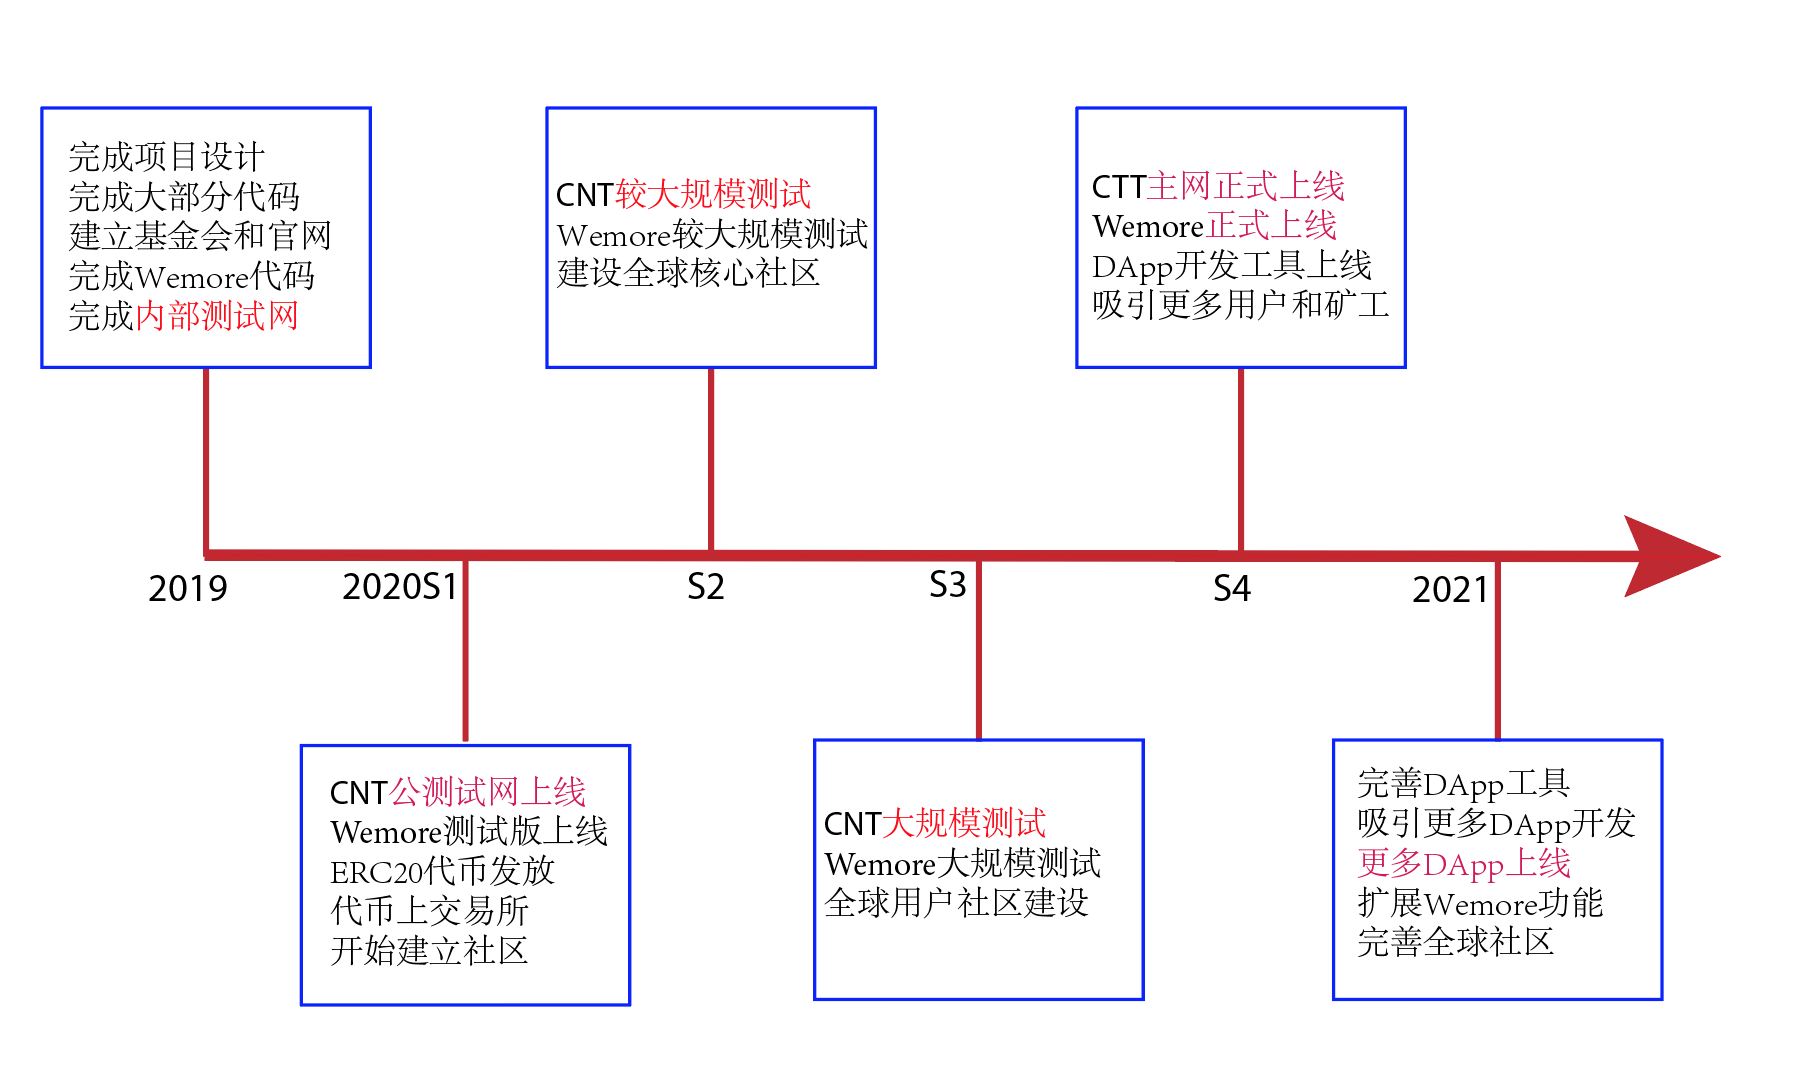
\includegraphics [width = 4in] {pic_cn/timeline.png}
\caption {CNT共识机制} \label {fig: timeline}
\end {figure}


\subsubsection{项目推广方法}

本项目将社区运营分为两方面:核心社区和外围社区,前者主要采用线下方式,后者主要采用线上模式 。在核心社区运营方面的计划是:

\begin{itemize}[itemindent=1em]
\item CNT基金会团队:我们将给团队一定的代币奖励,一是补偿前期投入的资源,二是让其能够成为权益关系人,期望未来继续投资持续参与CNT发展。
\item 区块链技术社区:技术是区块链发展的核心和难点。我们将利用创始团队的技术力量和社交资源, 以线上和线下两种方式,发掘、培育一批技术顶尖的人才,以促进技术社区的状大。
\item 区块链投资社区:以区块链技术社区为依托,通过投资人见面会的形式,我们即能向私募等投资社区的人士普及区块链知识,也能增进双方的合作机会。
\end{itemize}

\subsubsection{基金会管理和代币模型}

项目已经在新加坡成立非营利组织Contatract基金会,其目标是完善项目生态,促进项目愿景实现。代币是公有链生态系统不可缺少的组成部分。作为公有链经济系统的激励机制,它像是一个机械装置的润滑剂,又像生命系统的血液。正是以代币为基础的共识机制把社区成员聚集在一起,实现区块链生态系统良性循环。对于项目初创者,代币是对他们付出的必要的补偿和未来继续参与的动力;对于使用者,代币就是通行证;对于投资者,代币是通向未来的门票;对于开发者,代币让他们成为股东;对于记帐节点,代币更是他们辛勤付出的补偿。所有持有代币的人,他们可以是上述多重身份,他们与公有链项目息息相关,成为使用者、宣传者、开发者、投资者,与项目生态一起成长,成就CNT平台的伟大使命。基金会所有代币的私钥将由基金会决策委员会集体持有。这一方面避免独裁,另一方面避免单点风险。基金会决策委员会是基金会最高决策机关。

为了实现CNT平台的使命,CNT项目设计了Contatract(CNT)代币,并且设计了CNT代币的分布结构,以使项目可持续发展。代币在设计上主要考虑五个方面:

\begin{enumerate}
\item 数量。代币供应数量总共2的30次方,共计1073741824个,约10亿个。这个数量刚好是Contatract的世界硬盘管理单位,即一个存储组维护的空间大小为一个G。这个数量也能够使代币上线时有一个合理的价格,并在此基础上稳步成长,并使期在地球村阶段能够在数量表示上符合人们的习惯。
\item 代币发行机制。代币供应应该有个上限,实现非通胀的理念。这使越早参与者越有利,也使系统稳定性不断增强。
\item 代币分布。代币在分布上必须有很好的平衡,实现非中心的理念。CNT团队需要在通讯、数据存储、跨链和跨数据源上付出巨大的努力,我们分配10\%给核心团队,以支持到2030年之前的开发和运营。另外,因为CNT记帐节点任务比较重,可以占近三分之一。而剩余的将用于生态建设。
\item 生态建设。超过半数的代币将用于基金会,促进项目不断成长,特别在CNT宣传和应用生态上的建设需要大量的资金。
\item 矿工和燃料。各种价值将以分布式节点控制的方式进入到CNT,需要大量的分布式节点控制代币,节点越多安全性越高。并且在链上运行的价值越大,越需要更多的节点。要维持节点数量和算力,就需要给矿工记帐奖励和服务费。

\end{enumerate}

代币的分布如下:

\begin{enumerate}
\item 合伙人激励:10\%。用于参与从无到有创立该项目的合伙人,以及未来20年加入的对于项目有战略意义的合伙人的激励,绝大部分将长期锁定;
\item 开发者社区:5\%。项目未来将转入社区开发,以吸引顶尖的开发者加入,这部分代币将在未来20年分配给重要的开发者作为项目持续进步的奖励,绝大部分将长期锁定;
\item 代币互换:5\%。分配给愿意用其它代币换CNT的参与者,从而使团队获得流动性更强的代币用于支持早期开发和运营;
\item 生态建设:10\%。用于基金会合作发展,与区块链社区生态建设,在20年中逐渐释放,分配方法初步预计为在大地、小国、大国、地球村、深空等阶段各2\%;
\item 矿工奖励:70\%。将用于资源证明激励,其中存储挖矿和记账挖矿各占35\%。分20年完成,预计采用通胀率逐渐缩小的方式,具体办法将在公测后确定。
\end{enumerate}

在2020年,即主网上线之前流通的代币将以ERC20代币的形式存在。在主网上线之后将映射到主网中。

\section{结论}
人类文明还处于非常初级的阶段,其快速进步离不开各交易主体之间突破地理、制度、国家、组织等的限制进行深度合作。互联网的发展让人们看到了突破这些限制的希望。信息互联网已经使人们可以打破各种限制进行信息沟通,但越来越中心化的信息互联网需要转型为分布式信息互联网。价值互联网让人们看到打破各种限制进行价值交互的希望,但区块链的数据存储、跨链技术、可扩展能力还不足以支撑重的应用,区块链需要从图灵完备进化到功能完备。

Contatract致力于成为能够将信息互联网与价值互联网整合在以地址为核心的功能完备的、完全分布式并无限可扩展的公链系统。它通过主链分层分片使交易可以达到无限可扩展,通过多种功能子链及其分片使功能达到完备并无限可扩展。它以可读写存储功能子链为基础,使任何主体可以通过建立自己私有数据集的方式发布自己的身份信息、社交信息、富媒体、产品和智能合约,并通过这种方式在其上建立各种分布式应用程序。

Contatract是能够将区块链应用于社会方方面面的功能完备的第三代区块链。Contatrac基金会以社区为根本,采用分布式的治理机制,必将促使Contatract不断趋近自己的使命——通过建立以地址为核心的功能完备、完全分布式且无限可扩展的区块链促进人类高效合作。
%\theendnotes

\appendix
\clearpage
\renewcommand\refname{参考文献}
\bibliographystyle{Contatract}
\bibliography{Contatract}
\clearpage
%\renewcommand\appendixname{附录}

\end{document}

%%% Local Variables:
%%% mode: latex
%%% TeX-master: t
%%% End:
